\documentclass[krantz1,ChapterTOCs]{krantz}
\usepackage{fixltx2e,fix-cm}
\usepackage{amssymb}
\usepackage{amsmath}
\usepackage{graphicx}
\usepackage{subfigure}
\usepackage{makeidx}
\usepackage{multicol}
\usepackage[spanish]{babel}
\usepackage[utf8]{inputenc}
\usepackage{float}
\usepackage{yfonts}
\usepackage{amssymb}
\usepackage{minted}
\usemintedstyle{autumn}
\usepackage{mathtools,algorithm}
\usepackage[noend]{algpseudocode}
%\usepackage[dvips]{hyperref}

\frenchspacing
\tolerance=5000

\makeindex

\newtheorem{theorem}{Teorema}[chapter]
\newtheorem{exercise}{Exercise}[chapter]
\newtheorem{example}{Example}
\newtheorem{definition}{Definition}
\newtheorem{proof}{Proof}
 %place custom commands and macros here

\begin{document}

\frontmatter

\title{Modelos estocásticos y simulación 
%in Socio-Environmental Systems, Public Health, and Insurance\\
%{\Large(Applied Environmental Statistics Series)}
}
\author{Jorge Eduardo Ortiz Triviño}

\maketitle

%\cleardoublepage
\thispagestyle{empty}
\vspace*{\stretch{1}}
\begin{center}
\Large\itshape
To my dog\\
and my cat.
\end{center}
\vspace{\stretch{2}}
%\cleardoublepage
\setcounter{page}{1} %previous pages will be reserved for frontmatter to be added in later.
\tableofcontents
%\chapter*{Foreword}
I am delighted to introduce the first book on Multimedia Data Mining.  When I came to know about this book project undertaken by two of the most active young researchers in the field, I was pleased that this book is coming in early stage of a field that will need it more than most fields do.  In most emerging research fields, a book can play a significant role in bringing some maturity to the field.  Research fields advance through research papers.  In research papers, however, only a limited perspective could be provided about the field, its application potential, and the techniques required and already developed in the field.  A book gives such a chance.  I liked the idea that there will be a book that will try to unify the field by bringing in disparate topics already available in several papers that are not easy to find and understand.  I was supportive of this book project even before I had seen any material on it.  The project was a brilliant and a bold idea by two active researchers.  Now that I have it on my screen, it appears to be even a better idea.  

Multimedia started gaining recognition in 1990s as a field.  Processing, storage, communication, and capture and display technologies had advanced enough that researchers and technologists started building approaches to combine information in multiple types of signals such as audio, images, video, and  text.  Multimedia computing and communication techniques recognize correlated information in multiple sources as well as insufficiency of information in any individual source.    By properly selecting sources to provide complementary information, such systems aspire, much like human perception system, to create a holistic picture of a situation using only partial information from separate sources.

Data mining is a direct outgrowth of progress in data storage and processing speeds.  When it became possible to store large volume of data and run different statistical computations to explore all possible and even unlikely correlations among data, the field of data mining was born.  Data mining allowed people to hypothesize relationships among data entities and explore support for those.  This field has been put to applications in many diverse domains and keeps getting more applications.  In fact many new fields are direct outgrowth of data mining and it is likely to become a powerful computational tool.\vadjust{\vfill\pagebreak}



%\chapter*{Preface}
Approximately 17 million people in the USA (6{\%} of the
population) and 140 million people worldwide (this number is
expected to rise to almost 300 million by the year 2025) suffer
from \textit{diabetes mellitus}. Currently, there a few dozens of
commercialised devices for detecting blood glucose levels [1].
However, most of them are invasive. The development of a
noninvasive method would considerably improve the quality of life
for diabetic patients, facilitate their compliance for glucose
monitoring, and reduce complications and mortality associated with
this disease. Noninvasive and continuous monitoring of glucose
concentration in blood and tissues is one of the most challenging
and exciting applications of optics in medicine. The major
difficulty in development and clinical application of optical
noninvasive blood glucose sensors is associated with very low
signal produced by glucose molecules. This results in low
sensitivity and specificity of glucose monitoring by optical
methods and needs a lot of efforts to overcome this difficulty.

A wide range of optical technologies have been designed in
attempts to develop robust noninvasive methods for glucose
sensing. The methods include infrared absorption, near-infrared
scattering, Raman, fluorescent, and thermal gradient
spectroscopies, as well as polarimetric, polarization
heterodyning, photonic crystal, optoacoustic, optothermal, and
optical coherence tomography (OCT) techniques [1-31].

For example, the polarimetric quantification of glucose is based
on the phenomenon of optical rotatory dispersion, whereby a chiral
molecule in an aqueous solution rotates the plane of linearly
polarized light passing through the solution. The angle of
rotation depends linearly on the concentration of the chiral
species, the pathlength through the sample, and the molecule
specific rotation. However, polarization sensitive optical
technique makes it difficult to measure \textit{in vivo} glucose
concentration in blood through the skin because of the strong
light scattering which causes light depolarization. For this
reason, the anterior chamber of the eye has been suggested as a
sight well suited for polarimetric measurements, since scattering
in the eye is generally very low compared to that in other
tissues, and a high correlation exists between the glucose in the
blood and in the aqueous humor. The high accuracy of anterior eye
chamber measurements is also due to the low concentration of
optically active aqueous proteins within the aqueous humor.

On the other hand, the concept of noninvasive blood glucose
sensing using the scattering properties of blood and tissues as an
alternative to spectral absorption and polarization methods for
monitoring of physiological glucose concentrations in diabetic
patients has been under intensive discussion for the last decade.
Many of the considered  effects, such as changing of the size,
refractive index, packing, and aggregation of RBC under glucose
variation, are important for glucose monitoring in diabetic
patients. Indeed, at physiological concentrations of glucose,
ranging from 40 to 400 mg/dl, the role of some of the effects may
be modified, and some other effects, such as glucose penetration
inside the RBC and the followed hemoglobin glycation, may be
important [30-32].

Noninvasive determination of glucose was attempted using light
scattering of skin tissue components measured by a
spatially-resolved diffuse reflectance or NIR fre\-quen\-cy-domain
reflectance techniques. Both approaches are based on change in
glucose concentration, which affects the refractive index mismatch
between the interstitial fluid and tissue fibers, and hence
reduces scattering coefficient. A glucose clamp experiment showed
that reduced scattering coefficient measured in the visible range
qualitatively tracked changes in blood glucose concentration for
the volunteer with diabetes studied.




\listoffigures
%\listoftables
%%%\twocolumn
\chapter*{Contributors}

\begin{multicols}{2}
\contributor{Michael Aftosmis}{NASA Ames Research Center}{Moffett Field, California}

\contributor{Pratul K. Agarwal}{Oak Ridge National Laboratory}{Oak Ridge, Tennessee}

\contributor{Sadaf R. Alam}{Oak Ridge National Laboratory}{Oak Ridge, Tennessee}

\contributor{Gabrielle Allen}{Louisiana State University}{Baton Rouge, Louisiana}

\contributor{Martin Sandve Aln{\ae}s}{Simula Research Laboratory and University of Oslo, Norway}{Norway}

\contributor{Steven F. Ashby} {Lawrence Livermore National Laboratory}{Livermore, California}

\contributor{David A. Bader} {Georgia Institute of Technology}{Atlanta, Georgia}

\contributor{Benjamin Bergen} {Los Alamos National Laboratory}{Los Alamos, New Mexico}

\contributor{Jonathan W. Berry} {Sandia National Laboratories}{Albuquerque, New Mexico}

\contributor{Martin Berzins}{University of Utah}{Salt Lake City, Utah}

\contributor{Abhinav Bhatele}{University of Illinois}{Urbana-Champaign, Illinois}

\contributor{Christian Bischof} {RWTH Aachen University}{Germany}

\contributor{Rupak Biswas} {NASA Ames Research Center}{Moffett Field, California}\vspace*{5pt}

\contributor{Eric Bohm} {University of Illinois}{Urbana-Champaign, Illinois}\vspace*{5pt}

\contributor{James Bordner} {University of California, San Diego}{San Diego, California}\vspace*{5pt}

\contributor{George Bosilca} {University of Tennessee}{Knoxville, Tennessee}\vspace*{5pt}

\contributor{Greg L. Bryan} {Columbia University}{New York, New York}\vspace*{5pt}

\contributor{Marian Bubak} {AGH University of Science and Technology}{
Krak{\'o}w, Poland}\vspace*{5pt}

\contributor{Andrew Canning}{Lawrence Berkeley National
Laboratory}{Berkeley, California}

\contributor{Jonathan Carter} {Lawrence Berkeley National
Laboratory}{Berkeley, California}

\contributor{Zizhong Chen} {Jacksonville State University}{Jacksonville,
Alabama}

\contributor{Joseph R. Crobak} {Rutgers, The State University of New
Jersey}{Piscataway, New Jersey}

\contributor{Roxana E. Diaconescu} {Yahoo! Inc.}{Burbank, California}

\contributor{Peter Diener}
{Louisiana State University}{Baton Rouge, Louisiana}

\contributor{Jack J. Dongarra} {University of Tennessee, Knoxville, 
Oak Ridge National Laboratory, and}{University of Manchester}

\contributor{John B. Drake} {Oak Ridge National Laboratory}{Oak Ridge,
Tennessee}

\contributor{Kelvin K. Droegemeier} {University of Oklahoma}{Norman,
Oklahoma}

\contributor{St{\'e}phane Ethier} {Princeton University}{Princeton, New
Jersey}

\contributor{Christoph Freundl}
{Friedrich--Alexander--Universit{\"a}t}{Erlangen, Germany}

\contributor{Karl F{\"u}rlinger} {University of Tennessee}{Knoxville,
Tennessee}

\contributor{Al Geist} {Oak Ridge National Laboratory}{Oak Ridge,
Tennessee}

\contributor{Michael Gerndt} {Technische Universit{\"a}t
M{\"u}nchen}{Munich, Germany}

\contributor{Tom Goodale}
{Louisiana State University}{Baton Rouge, Louisiana}

\contributor{Tobias Gradl}
{Friedrich--Alexander--Universit{\"a}t}{Erlangen, Germany}

\contributor{William D. Gropp} {Argonne National Laboratory}{Argonne,
Illinois}

\contributor{Robert Harkness} {University of California, San
Diego}{San Diego, California}

\contributor{Albert Hartono} {Ohio State University}{Columbus, Ohio}

\contributor{Thomas C. Henderson} {University of Utah}{Salt Lake City,
Utah}

\contributor{Bruce A. Hendrickson} {Sandia National
Laboratories}{Albuquerque, New Mexico}

\contributor{Alfons G. Hoekstra} {University of Amsterdam}{Amsterdam,
The Netherlands}

\contributor{Philip W. Jones} {Los Alamos National Laboratory}{Los
Alamos, New Mexico}

\contributor{Laxmikant Kal{\'e}} {University of
Illinois}{Urbana-Champaign, Illinois}

\contributor{Shoaib Kamil} {Lawrence Berkeley National
Laboratory}{Berkeley, California}

\contributor{Cetin Kiris} {NASA Ames Research Center}{Moffett Field,
California}

\contributor{Uwe K{\"u}ster} {University of Stuttgart}{Stuttgart,
Germany}

\contributor{Julien Langou} {University of Colorado}{Denver, Colorado}

\contributor{Hans Petter Langtangen}
{Simula Research Laboratory and}{University of Oslo, Norway}

\contributor{Michael Lijewski} {Lawrence Berkeley National
Laboratory}{Berkeley, California}

\contributor{Anders Logg}
{Simula Research Laboratory and}{University of Oslo, Norway}

\contributor{Justin Luitjens} {University of Utah}{Salt Lake City, Utah}

\contributor{Kamesh Madduri} {Georgia Institute of Technology}{Atlanta,
Georgia}

\contributor{Kent-Andre Mardal}
{Simula Research Laboratory and}{University of Oslo, Norway}

\contributor{Satoshi Matsuoka} {Tokyo Institute of Technology}{Tokyo,
Japan}

\contributor{John M. May} {Lawrence Livermore National
Laboratory}{Livermore, California}

\contributor{Celso L. Mendes} {University of Illinois}{Urbana-Champaign,
Illinois}

\contributor{Dieter an Mey} {RWTH Aachen University}{Germany}

\contributor{Tetsu Narumi} {Keio University}{Japan}

\contributor{Michael L. Norman} {University of California, San
Diego}{San Diego, California}

\contributor{Boyana Norris} {Argonne National Laboratory}{Argonne,
Illinois}

\contributor{Yousuke Ohno} {Institute of Physical and Chemical Research
(RIKEN)}{Kanagawa, Japan}

\contributor{Leonid Oliker} {Lawrence Berkeley National
Laboratory}{Berkeley, California}

\contributor{Brian O'Shea} {Los Alamos National Laboratory}{Los Alamos,
New Mexico}

\contributor{Christian D. Ott}
{University of Arizona}{Tucson, Arizona}

\contributor{James C. Phillips} {University of
Illinois}{Urbana-Champaign, Illinois}

\contributor{Simon Portegies Zwart} {University of
Amsterdam,}{Amsterdam, The Netherlands}

\contributor{Thomas Radke}
{Albert-Einstein-Institut}{Golm, Germany}

\contributor{Michael Resch} {University of Stuttgart}{Stuttgart,
Germany}

\contributor{Daniel Reynolds} {University of California, San Diego}{San
Diego, California}

\contributor{Ulrich R{\"u}de}
{Friedrich--Alexander--Universit{\"a}t}{Erlangen, Germany}

\contributor{Samuel Sarholz}
{RWTH Aachen University}{Germany}

\contributor{Erik Schnetter}
{Louisiana State University}{Baton Rouge, Louisiana}

\contributor{Klaus Schulten} {University of Illinois}{Urbana-Champaign,
Illinois}

\contributor{Edward Seidel}
{Louisiana State University}{Baton Rouge, Louisiana}

\contributor{John Shalf} {Lawrence Berkeley National
Laboratory}{Berkeley, California}

\contributor{Bo-Wen Shen} {NASA Goddard Space Flight Center}{Greenbelt,
Maryland}

\contributor{Ola Skavhaug}
{Simula Research Laboratory and}{University of Oslo, Norway}

\contributor{Peter M.A. Sloot} {University of Amsterdam}{Amsterdam, The
Netherlands}

\contributor{Erich Strohmaier} {Lawrence Berkeley National
Laboratory}{Berkeley, California}

\contributor{Makoto Taiji} {Institute of Physical and Chemical Research
(RIKEN)}{Kanagawa, Japan}

\contributor{Christian Terboven}
{RWTH Aachen University,}{Germany}

\contributor{Mariana Vertenstein} {National Center for Atmospheric
Research}{Boulder, Colorado}

\contributor{Rick Wagner} {University of California, San Diego}{San
Diego, California}

\contributor{Daniel Weber} {University of Oklahoma}{Norman, Oklahoma}

\contributor{James B. White, III} {Oak Ridge National Laboratory}{Oak
Ridge, Tennessee}

\contributor{Terry Wilmarth} {University of Illinois}{Urbana-Champaign,
Illinois}

\end{multicols}
%\chapter*{Symbols}
\begin{symbollist}{000000}
\symbolentry{$\alpha$}{To solve the generator maintenance scheduling, in the  past, several mathematical techniques have  been applied.}
\symbolentry{$\sigma^2$}{These include integer programming, integer linear programming, dynamic programming, branch and bound etc.}
\symbolentry{$\sum$}{Several heuristic search algorithms have also been developed. In recent years expert systems,}
\symbolentry{$abc$}{fuzzy approaches, simulated annealing and genetic algorithms have also been tested.}
\symbolentry{$\theta\sqrt{abc}$}{This paper presents a survey of the literature}
\symbolentry{$\zeta$}{ over the past fifteen years in the generator}
\symbolentry{$\partial$}{maintenance scheduling. The objective is to}
\symbolentry{sdf}{present a clear picture of the available recent literature}
\symbolentry{ewq}{of the problem, the constraints and the other aspects of}
\symbolentry{bvcn}{the generator maintenance schedule.}
\end{symbollist}

\mainmatter
\part{MODELOS ESTOCÁSTICOS}
\chapter{INTRODUCCIÓN}
\chapter{ALGUNOS EJEMPLOS}

\part{VARIABLES Y VECTORES ALEATORIOS}

\chapter{ESPACIOS DE PROBABILIDAD}
\chapter{ESPACIOS DE PROBABILIDAD CONDICIONAL}
\chapter{VARIABLES ALEATORIAS}
\chapter{VECTORES ALEATORIOS}
\chapter{TRANSFORMACIONES DE VECTORES ALEATORIOS}


\part{PROCESOS ESTOCÁSTICOS Y SERIES DE TIEMPO}

\chapter{PROCESOS ESTOCÁSTICOS}

%Laura Morales Ariza
\newpage

En este capítulo se presentan los sistemas de ecuaciones lineales en diferencias estocásticos como modelos para describir las dinámicas internas y cruzadas entre las series de tiempo obtenidas del sistema dinámico $S$ en estudio. Aunque los modelos parten del supuesto de linealidad, las series
modeladas no tienen por qué serlo. Los mismos modelos incorporan mecanismos propios que permiten, a través de \textit{transformaciones}, estudiar y analizar conjuntos de series de tiempo que no presentan esta característica.

Existen otros tipos de modelos, tales como las redes neuronales artificiales (entre otros), que no suponen tal comportamiento lineal sobre los datos; sin embargo, ambos puntos de vista, el enfoque presentado aquí, usualmente conocido como \textit{análisis clásico de series de tiempo} y el \textit{análisis contemporáneo inspirado en el funcionamiento del cerebro humano} tienen ventajas y desventajas.
En tal virtud le corresponde al experto definir cuál de los dos debe emplear de acuerdo con la
situación particular.

El esquema y notación empleados en este documento están basados en  \cite{trivino2012esthocasticModels};\cite{wei1994timeseries}, en esos textos se detallan con mayor profundidad los resultados aquí presentados.


\section{INTRODUCCIÓN}\label{sec:intro1}
\setcounter{equation}{0}

Una \textit{serie de tiempo} es una secuencia ordenada de observaciones o, formalmente, una realización de
un proceso estocástico. Aunque el orden se hace usualmente a través del tiempo (en el sentido
cronológico), sobre todo en términos de algunos intervalos de tiempo equidistantes, el orden
también se puede tomar a través de otras dimensiones, como el espacio y más específicamente el
\textit{espacio-tiempo}. Las series de tiempo se producen en una variedad de campos. En la agricultura, se
observa precios diarios de cierre de acciones, tasas de interés, precios semanales índices mensuales,
las ventas trimestrales y ganancias anuales. En ingeniería, observamos sonido, señales eléctricas, y
el voltaje. En geofísica, registramos la turbulencia, como las olas del mar y el ruido de la tierra en un
área. En estudios médicos, medimos el trazado del electroencefalograma (EEG) y el
electrocardiograma (ECG). En meteorología, observamos velocidades por hora de viento,
temperatura diaria y las precipitaciones anuales. En el control de calidad, hacemos un seguimiento
de un proceso de acuerdo con un determinado valor objetivo. En ciencias sociales, se estudian las tasas anuales de natalidad, tasas de mortalidad, las tasas de accidentes, y varios índices de
criminalidad. La lista de las áreas en las que se observa la serie de tiempo y estudió es aún más
grande. En general, en el modelamiento de un sistema (complejo) $S$ concurren series de todas estas
disciplinas y, probablemente, muchas más; por ejemplo, índices de calidad de vida, series de tiempo
de impacto ambiental, datos cronológicos de catástrofes naturales, etc. Por tal razón se hace
necesario emplear instrumentos matemáticos apropiados que permitan describir la dinámica
subyacente en los datos como las relaciones entre las diferentes series y construir instrumentos que
permitan predecir valores o comportamientos futuros con unos niveles de error aceptados.\\


Hay diversos objetivos para el estudio de series de tiempo. Ellos incluyen la comprensión y
descripción del mecanismo de generación, la predicción o pronóstico de valores futuros, y un
control óptimo de sistema. La naturaleza intrínseca de una serie de tiempo es que sus observaciones
son dependientes o correlacionados, y el orden de las observaciones es por lo tanto importante. Por
lo tanto, los procedimientos estáticos y técnicas que se basan en hipótesis de independencia ya no
son aplicables, y, en consecuencia se hace necesario el empleo de otro tipo de métodos. El cuerpo de
la metodología estadística disponible para el análisis de series de tiempo se conoce como análisis de
series de tiempo. Y ese es el propósito de este documento, realizar un esbozo general pero no
profundo de tales técnicas.\\


En este capítulo, se presentan algunos conceptos fundamentales que son necesarios para la adecuada
comprensión de los modelos de series de tiempo que se incluyen en este documento. Las dinámicas
se describen a través de sistemas de ecuaciones en diferencias estocásticas lineales homogéneas con
coeficientes constantes. Se presentan las funciones de autocorrelación y autocorrelación parcial y la
noción de ruido blanco, y también los estimadores de la media, la autocovarianza y la correlación.
Con base en esas estimaciones se describe el método de identificación de los modelos.

\section{ECUACIONES EN DIFERENCIAS LINEALES HOMOGÉNEAS}\label{sec:ecuac} 

\subsection{Operador de retardo y de diferencias}

Dada una serie $X_{t}$, el operador de retardo $B$, que se ilustra en la Figura \arabic{chapter}.1, atrasa en una unidad
la serie de tiempo, es decir $X_{t-1} = BX_{t}$. Este operador puede generalizarse para que desfase la serie $k$ unidades de tiempo. Este hecho se escribe formalmente como $X_{t-k} = B^{k} X_{t}$ y se representa esquemáticamente en la Figura \arabic{chapter}.2.

\begin{figure}[H]
     \begin{center}
         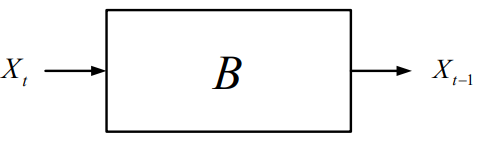
\includegraphics[width=100mm]{chapters/chapter2/figures/operadorretardo.PNG}
     \end{center}
     \textbf{\caption{Operador de retardo}}
     \label{fig:1}
\end{figure}

\begin{figure}[H]
     \begin{center}
         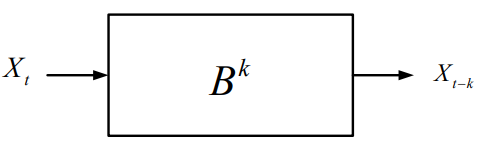
\includegraphics[width=100mm]{chapters/chapter2/figures/operadorretardotiempo.PNG}
     \end{center}
     \textbf{\caption{Operador de retardo de k unidades de tiempo}}
\end{figure}

De forma similar el operador de diferencias trabaja de la forma descrita en la Figura \arabic{chapter}.3, es decir, dada la serie $\dot{X}_{t}$ su \textit{d ésima} diferencia está dada por $X_{t} = (1-B)^d$ $\dot{X}_{t} = \sum_{k=0}^d {d \choose k} (-1)^{d-k} \dot{X}_{d-k}$.

\begin{figure}[H]
     \begin{center}
         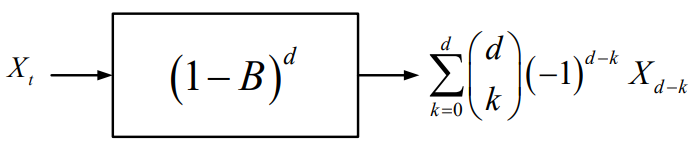
\includegraphics[width=120mm]{chapters/chapter2/figures/operadordiferencias.PNG}
     \end{center}
     \textbf{\caption{Operador de diferencias}}
\end{figure}

\subsection{Solución general de una ecuación en diferencias lineal homogénea}

****No hay contenido *****

\section{PROCESOS ESTOCÁSTICOS Y SERIES DE TIEMPO}\label{sec:procestoc}

Un proceso estocástico se define matemáticamente como un conjunto de variables aleatorias $\{X_{t_{i}}\}^{i=n}_{i=1}$ que siguen la distribución conjunta de la ecuación \ref{onePoint} donde $\{x_{i}\}^{i=n}_{i=1} \in \mathbb{R}^n$.

\begin{equation}
F_{X_{t_{1}},X_{t_{2}},...,X_{t_{n}},} (X_{1},X_{2},...,X_{n}) = P[w: X_{t_{1}} \leq x_{1},X_{t_{2}} \leq x_{2},...,X_{t_{n}} \leq x_{n}]
\label{onePoint}
\end{equation}
\\

Por su parte una serie de tiempo es una realización de un proceso estocástico. Es decir, es un
conjunto de valores $\{x_{i}\}^{i=n}_{i=1} \in \mathbb{R}^n$ que han sido tomados de la distribución conjunta (\ref{onePoint}).

Por ejemplo, como resultado del proceso de simulación en el prototipo del sistema en estudio $S$ se obtienen decenas de tablas con series de tiempo similares a las presentadas en la Figura \arabic{chapter}.4 (donde
solamente aparecen dos tablas). Esos datos pueden ser representados en un sistema cartesiano como
el de la Figura \arabic{chapter}.5.

\begin{figure}[H]
     \begin{center}
         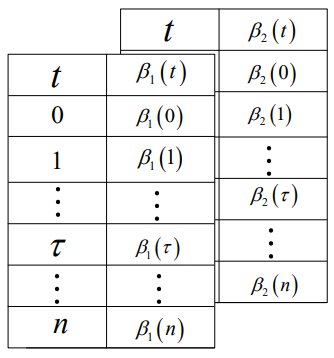
\includegraphics[width=70mm]{chapters/chapter2/figures/dosseriestiempo.PNG}
     \end{center}
     \textbf{\caption{Dos series de tiempo de dos indicadores en el sistema $S$}}
\end{figure}

\begin{figure}[H]
     \begin{center}
         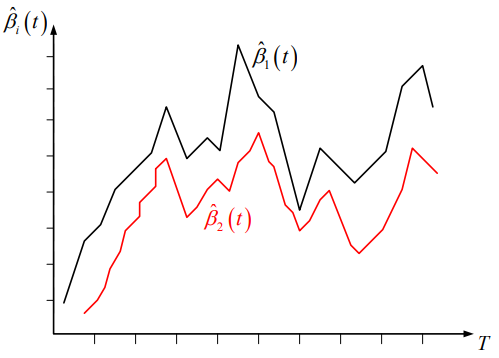
\includegraphics[width=100mm]{chapters/chapter2/figures/mateseriestiempo.PNG}
     \end{center}
     \textbf{\caption{Representación matemática de las series de tiempo de dos indicadores}}
\end{figure}

\section{FUNCIONES DE AUTOCOVARIANZA, AUTOCORRELACIÓN Y AUTOCORRELACIÓN PARCIAL}\label{sec:autovar}

\subsection{Definiciones formales}

Para un proceso estacionario $\{X_{t}\}^{t=n}_{t=1}$, la media $E(X_{t}) = \mu_{X}$ y la varianza $\sigma^{2}_{X} = Var(X_{t}) = E(X_{t}-\mu_{X})^2 $ son constantes, y las covarianzas $Cov(X_{t},X_{s})$, son funciones
únicamente de la diferencia de tiempo $k=|t-s|$. Por lo tanto, en este caso, se describe la covarianza
entre $X_{t}$ y $X_{t+k}$ de acuerdo con la ecuación (\ref{twoPoint}).

\begin{equation}
\gamma_{k} = Cov(X_{t},X_{s}) =  E(X_{t}-\mu_{X})(X_{t+k}-\mu_{X})
\label{twoPoint}
\end{equation}
\\

Y la correlación entre $X_{t}$ y $X_{t+k}$ como se presenta en la ecuación (\ref{threePoint}).

\begin{equation}
\rho_{k} = \frac{Cov(X_{t},X_{t+k})}{\sqrt{Var(X_{t})} \sqrt{Var(X_{t+k})}} = \frac{\gamma_{k}}{\gamma_{0}}
\label{threePoint}
\end{equation}
\\

donde $\sigma^{2}_{X} = Var(X_{t}) = Var(X_{t+k}) = \gamma_{0}$. Como funciones de $k$, $\gamma_{k}$ se denomina función de autocovarianza y $\rho_{k}$ se llama función de autocorrelación (ACF) en el análisis de series de tiempo, ya que representan la covarianza y la correlación entre $X_t$ y $X_{t+k}$ desde el mismo proceso, separadas únicamente por $k$ unidades de tiempo. Una función de autocorrelacion típica se presenta en la Figura \arabic{chapter}.6.

Además de la autocorrelación entre $X_t$ y $X_{t+k}$, se requiere conocer la correlación entre $X_t$ y $X_{t+k}$ dado que se conocen los valores de las variables aleatorias $X_{t+1},X_{t+2},...,$ y $X_{t+k-1}$. En términos
matemáticos esto se expresa mediante la ecuación (\ref{fourPoint}).

\begin{equation}
\phi_{kk} = Corr(Z_t,Z_{t+k}|Z_{t+1},...,Z_{t+k-1})
\label{fourPoint}
\end{equation}
\\

\begin{figure}[H]
     \begin{center}
         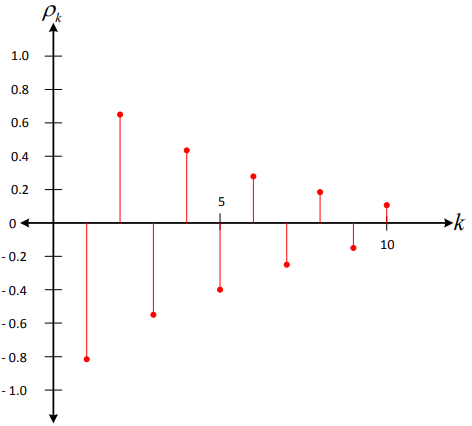
\includegraphics[width=90mm]{chapters/chapter2/figures/fautocorrelacion.PNG}
     \end{center}
     \textbf{\caption{Una función de autocorrelación típica}}
\end{figure}


La expresión (\ref{fourPoint}) se refiere generalmente como la autocorrelación parcial en el análisis de series
de tiempo. Puede demostrarse que la expresión (\ref{fourPoint}) es equivalente a la ecuación (\ref{fivePoint}).

\begin{equation}
\phi_{11} = \rho_{1}
\label{fivePoint}
\end{equation}
\\

\begin{equation*}
\phi_{kk} =  \frac{
\left| 
\begin{array}{cccccc}
1 & \rho_{1} & \rho_{2} & \cdots & \rho_{k-2} & \rho_{1} \\
\rho_{1} & 1 & \rho_{1} & \cdots & \rho_{k-3} & \rho_{2} \\
\vdots & \vdots & \vdots & \ddots & \vdots & \vdots\\
\rho_{k-1} & \rho_{k-2} & \rho_{k-3} & \cdots & \rho_{1} & \rho_{k} \\
\end{array}
\right|}{
\left| 
\begin{array}{cccccc}
1 & \rho_{1} & \rho_{2} & \cdots & \rho_{k-2} & \rho_{k-1} \\
\rho_{1} & 1 & \rho_{1} & \cdots & \rho_{k-3} & \rho_{k-2} \\
\vdots & \vdots & \vdots & \ddots & \vdots & \vdots\\
\rho_{k-1} & \rho_{k-2} & \rho_{k-3} & \cdots & \rho_{1} & 1 \\
\end{array}
\right|
} 
\end{equation*}
\\

\chapter{SERIES DE TIEMPO}
\chapter{CADENAS DE MARKOV}



\part{TEORÍA DE TELETRÁFICO}
\chapter{SISTEMA DE COLAS SIMPLES}

\section{INTRODUCCIÓN}\label{intro}
En este capítulo se presenta el principal modelo de colas simples. En capítulos posteriores se
discutirán las redes de colas que son la extensión del modelo simple aquí estudiado. El modelo de
colas simple es el ladrillo a partir del cual se construye el edificio de la planeación de redes y el
análisis de desempeño en los sistemas de telecomunicaciones. La mayoría de trabajos de modelado
que se han hecho para sistemas de colas involucra, necesariamente, al menos una cola simple. La
principal razón es que para cualquier investigación en la teoría de colas, el sistema de cola simple es
un punto de partida natural. Otra razón es la facilidad de su tratamiento: Es mucho más fácil
formalizar los resultados con una cola simple para luego extenderlo a modelos más complejos de
red de colas.
\\
En particular, aquí se estudian los fundamentos del sistema de colas básico, llamado $( M/M/1)$: Este es un modelo de colas “Markoviano” en el que se distingue un proceso de llegada de Poisson y
tiempo de servicio exponencial. Para representar la dinámica de ese sistema se emplean los
diagramas de transición de estados.


\section{EXPRESIÓN DE KENDALL Y MEDIDAS DE DESEMPEÑO.}\label{intro}
\subsection{Notación.}
Para referirse formalmente a los principales elementos matemáticos que hacen parte de un sistema
de líneas de espera (o colas) es ampliamente aceptada la notación de seis (6) parámetros propuesta
por Kendall. En dicha convención se expresa un sistema de líneas de espera mediante el siguiente formato de la expresión \ref{eqn:1.1}.

\begin{equation}
    \left( a/b/c \right) :\left( d/e/f \right)
    \label{eqn:1.1}
\end{equation}
\\
Cada uno de los tres parámetros que conforman las dos secciones presentes en la expresión \ref{eqn:1.1}
tienen un significado asociado. En la primera sección, el parámetro {\em a} representa la estructura (o familia) probabilística que guía la llegada de clientes al sistema; el parámetro {\em b} se emplea para
indicar la estructura probabilística del tiempo de atención por parte del servidor o de los servidores.
Ellos usualmente se sustituyen por las letras mayúsculas {\em M} que indica {\em “Markoviano”} y que implica que el número de clientes corresponde a un proceso de {\em Poisson}; la letra
{\em D} significa {\em “determinístico”} o {\em “degenerado”} queriendo decir que los tiempos de llegada (o atención según el caso) son constantes y no variables aleatorias. La letra {\em G} se utiliza para indicar que la familia probabilística es {\em “general”} es decir cualquiera. Por su lado, el último parámetro de la primera sección, \(c \in \mathbb{N}\)
, es una constante natural que indica el número de servidores en paralelo que trabajan
en el sistema (usualmente $ c = 1 $).
\\
Los parámetros de la segunda sección de la referida expresión también tienen sus significados
específicos. El parámetro {\em d} se emplea para indicar la disciplina de servicio; esto es, el mecanismo
que empleará el servidor para seleccionar al siguiente cliente que él va a atender una vez se
desocupe del cliente que está actualmente atendiendo. Este parámetro es frecuentemente FIFO
(primero en llegar primero en ser atendido); sin embargo, hay otras opciones. Por ejemplo LIFO
(último en llegar, primero en ser atendido). Por su parte, el parámetro $ c \in \mathbb{N} $ representa la capacidad del sistema; es decir, el número máximo de clientes (simultáneos) que pueden permanecer dentro del
sistema. Finalmente, el tamaño de la población, origen de los clientes, lo representa el parámetro {\em f}.
\\
\\
\textbf{Ejemplo 1—1: Un sistema de líneas de espera.}

La expresión (Cauchy$(\alpha,\beta )$/Uniforme$( \eta ,\mu  )$/7):(LIFO/180/1.000.000) describe un sistema de líneas de espera con tiempos entre llegadas de la familia Cauchy, tiempo de atención en los 7 servidores en paralelo de la familia uniforme. Política de atención LIFO, máximo 180 clientes dentro del sistema (capacidad de la fila 180-7=173) y tamaño de la población de donde provienen los clientes de un millón.
\\
\textbf{\textit{Observación:}}
Cuando en esta nomenclatura se suprime la segunda sección se supone: Política FIFO, Capacidad
del sistema y tamaño de la población infinitos. Esquemáticamente eso significa:
\begin{equation}
    \left ( a/b/c \right ) = \left ( a/b/c \right ) : \left ( FIFO/+\infty/+\infty\right )
    \label{eqn:1.2}
\end{equation}

\subsection{Medidas de desempeño.}
Especificar el sistema no es suficiente. A partir de esa especificación formal se deben obtener medidas que describan de alguna manera el comportamiento o desempeño de ese sistema. Aunque esas medidas de desempeño pueden ser de diferentes formas y de distintas propiedades, es frecuente intentar calcular: (1) El número medio de clientes en el sistema, (2) El número de clientes esperado en fina, (3) El tiempo promedio dentro del sistema, (4) El tiempo medio de permanencia en cola
(fila) y (5) La utilización, que se define como el porcentaje de tiempo que los servidores permanecen ocupados. Aquí solo nombramos cinco pero la lista puede crecer tanto como se quiera.

\begin{figure}[H]
\centering
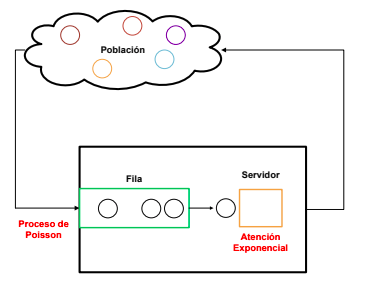
\includegraphics[width=3in]{chapters/chapter3/figures/Figura1-1:Sistema(mm1).png}
%%\centerline{\epsfig{/Chapters/chapter3/figures/Figura1-1:Sistema(mm1).png,width=.8\textheight,height=.4\textwidth}}
\caption[Sistema (M/M/1)]{Sistema (M/M/1)}
\label{fig:mesh1}
\end{figure}

\section{SISTEMA DE COLAS \textit{(M/M/1)}}
Considérese el sistema de la Figura \ref{fig:mesh1}. Ese es el sistema de colas simple del cual parte la teoría de colas. El sistema $(M/M/1)$ tiene dos supuestos importantes. El primero es que el proceso de llegadas es un proceso de Poisson, y el otro que cuenta con un único servidor razón por la cual tiene un único tiempo de servicio que corresponde a una variable con distribución exponencial. Estos supuestos llevan a un modelo muy manejable y además razonable, para una gran variedad de situaciones. Se examinarán ahora estos dos supuestos.
\subsection {Procesos binomiales y Procesos de Poisson.}
El $proceso$ $de$ $Poisson$ es el proceso de llegada más sencillo. Una forma de entenderlo es esta. Suponga que el eje temporal se divide en un gran número de pequeños segmentos de longitud
$ \Delta t $. Se supone que la probabilidad de que un único cliente llegue a un segmento es proporcional a la
longitud de ese segmento,$ \Delta t $, multiplicado por una constante de proporcionalidad, multiplicado por una constante de proporcionalidad, $ \lambda $, que representa la tasa media de llegadas:
\begin{equation}
    P\left [ Exactamente \; 1 \; llegada \;en \left [ t,t+\Delta t \right ] \right ] = \lambda \Delta t
    \label{eqn:1.3}
\end{equation}

\begin{equation}
    P\left [ No \;llega \;en  \left [ t,t+\Delta t \right ] \right ] = 1-\lambda \Delta t
    \label{eqn:1.4}
\end{equation}

\begin{equation}
    P\left [ M\acute{a}s\; de \; 1 \; llegada\; en  \left [ t,t+\Delta t \right ] \right ] = 0
    \label{eqn:1.5}
\end{equation}
\\
Aquí (dada su magnitud) se ignoran los términos de orden superior que involucren $ \Delta t $. Es posible hacer una analogía entre el proceso de llegada y el lanzamiento de una moneda en cada uno de los segmentos. Aquí la probabilidad de llegada es $ \lambda \Delta t $ (es decir, cara) y $1-\lambda \Delta t$ es la probabilidad de
no llegada (es decir, sello). Los lanzamientos, y en consecuencia los resultados, de cada moneda son, a simple vista, independientes unos con otros; por esta razón, al observar el comportamiento del sistema en un intervalo de tiempo $\left [ 0,t \right )$ en el cual se pueda escribir $t = n\Delta t $ con $ c \in \mathbb{N} $ y, en consecuencia, $ t \in \mathbb{R}^{+} $ , es claro que al definir la variable aleatoria $ N_{t} $ como el número de clientes que arriban al sistema en $ \left [ 0,t \right ) $ su estructura probabilística es $ N_{t} \sim Binomial \left ( n,p=\lambda \Delta t \right ) $ o, más específicamente, $ f_{N_{t}}\left ( k;n,p=\lambda \Delta t \right ) = P \left [ N_{t} = k \right ] $ , está dada en la ecuación \ref{eqn:1.6}.

\begin{equation}
    f_{N_{t}}\left ( k;n,p=\lambda \Delta t \right ) = \binom{n}{k}\left ( \lambda \Delta t \right )^{k}\left ( 1 - \lambda \Delta t \right )^{1-k}
    \label{eqn:1.6}
\end{equation}
\\
De ahí que la estructura probabilística dependa del tiempo de observación del sistema $ t $ y que, por lo tanto, rigurosamente hablando, a este modelo se le conozca con el nombre de \textit{Procesos estocásticos binomiales de nacimiento puro}. Cuando $ \Delta t \rightarrow 0 $ se obtiene un proceso de Poisson de tiempo continúo puesto que, como se mostrará más adelante, una familia binomial converge a una familia de Poisson cuando $ n \rightarrow 0 $, $ p=\lambda \Delta t  \rightarrow 0 $ y $ \mu _{N_{t}}= p \times n = \lambda $  permanece constante. En este escenario, cada lanzamiento de una moneda puede ser una analogía de las llegadas, unas independientes de otras, ya que se puede pensar en un simple resultado positivo de una larga lista de lanzamientos de monedas independientes. Además, se puede ver todos los intervalos de tiempo tienen la misma probabilidad constante de tener una llegada.


\begin{figure}[H]
\centering
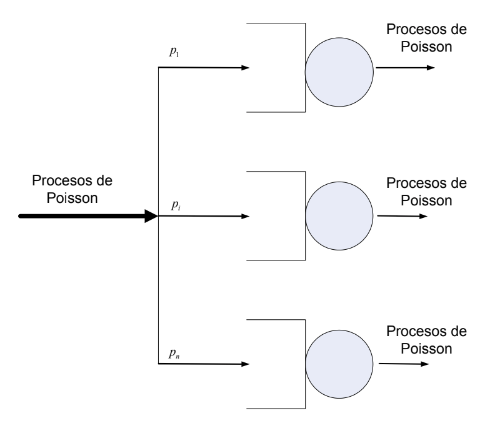
\includegraphics[width=3in]{chapters/chapter3/figures/Figura1-2:BifurcaciondeunprocesodePoisson.png}
%%\centerline{\epsfig{/Chapters/chapter3/figures/Figura1-1:Sistema(mm1).png,width=.8\textheight,height=.4\textwidth}}
\caption[Bifurcación de un proceso de Poisson]{Bifurcación de un proceso de Poisson}
\label{fig:mesh2}
\end{figure}

\subsection{Dos propiedades importantes de los procesos de Poisson.}
Dos ideas importantes caracterizan a los procesos de Poisson. La primera es el proceso de bifurcación aleatoria de un proceso de Poisson y la segunda es la unión de varios procesos de Poisson. La Figura \ref{fig:mesh2} ilustra un sistema de filas con variables ramificación o bifurcaciones. La llegada se divide aleatoriamente entre $ n $ ramas con probabilidades independientes $ p_{1},\cdots,p_{i},\cdots, p_{n} $. La segunda, que se ilustra en la Figura \ref{fig:mesh3}, es una situación que envuelve la unión de procesos de Poisson independientes. En este caso, las llegadas de un número de procesos independientes se unen o fusionan en un único proceso agregado.
Una de las aplicaciones originales, aunque no la única ni la más importante, de los procesos de Poisson en redes de comunicaciones es el modelo de llegadas de llamadas a una central telefónica. 

El uso de cada teléfono, por lo menos en un primer análisis, puede ser modelado por un proceso de Poisson. Así, modelar puede convertirse en algo complicado, pero es indudable la elegancia de formular este tipo de modelos para realizar planeación de redes de computadores y de telecomunicaciones de una manera formal y bella. El punto importante está en que tanto los procesos de ramificaciones aleatorias como las uniones de procesos de Poisson resultan ser también Procesos de Poisson. La analogía del lanzamiento de monedas sirve para demostrar de una manera muy sencilla que estos resultados son verdad.

\begin{figure}[H]
\centering
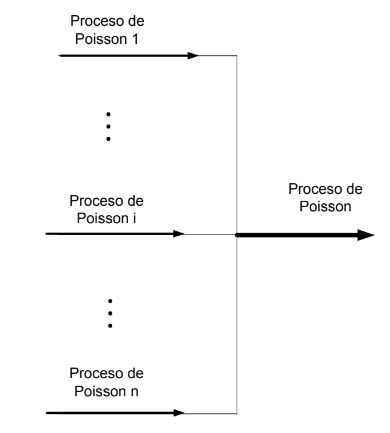
\includegraphics[width=2in]{chapters/chapter3/figures/Figura1-3:UniondeVariosprocesosdePoisson.png}
%%\centerline{\epsfig{/Chapters/chapter3/figures/Figura1-1:Sistema(mm1).png,width=.8\textheight,height=.4\textwidth}}
\caption[Unión de varios procesos de Poisson]{Unión de varios procesos de Poisson}
\label{fig:mesh3}
\end{figure}

\subsection{Fundamentos del proceso de Poisson.}
En este apartado se deduce una ecuación diferencial que se obtiene del proceso de Poisson a partir del modelo discreto resulta de partir de pequeños intervalos $ \Delta t $ de tiempo para, finalmente, tomar
el límite cuando $ \Delta t \rightarrow 0 $. En primer lugar

\begin{equation}
    P_{n}\left ( t \right ) = P \left ( \#\; llegan = n\; en\; tiempo\; t \right )
    \label{eqn:1.7}
\end{equation}
\\
Además, sea $ P_{ij}\left (  \Delta t \right ) $ la probabilidad de pasar de $i$ llegadas (nacimientos) a $j$ en $ \Delta t$ segundos.El proceso de deducción que aquí se presenta está inspirado en el libro \cite{kleinrock1975}. En este modelo, el número de llegadas (o nacimientos) es el “estado” del sistema. Este dato contiene toda la información necesaria para describir el sistema de una manera adecuada. Dicho esto, es claro, entonces que para esta situación se cumple la ecuación \ref{eqn:1.8}

\begin{equation}
    P_{n}\left ( t + \Delta t \right ) = P_{n}\left ( t \right )P_{n,n}\left ( \Delta t \right )+P_{n-1}\left ( t \right )P_{n-1,n}\left ( \Delta t \right )
    \label{eqn:1.8}
\end{equation}
\\
Nuevamente aquí, no se tiene en cuenta (por ser de magnitudes muy pequeñas) los términos de orden superior en $ \Delta t $. Lo que dice la ecuación \ref{eqn:1.8} es que el sistema puede llegar al estado $n$, esto tener clientes o nacimiento en el tiempo en el intervalo $ \left [ 0,t + \Delta t \right ) $ ya sea porque en el intervalo $ \left [ 0,t \right ) $ el sistema ya se encontraba en el estado $ n $ y que durante el intervalo $ \left [ t,t + \Delta t \right ) $ no haya habido ninguna llegada, o bien, que en el intervalo $ \left [ 0,t \right ) $ el sistema estaba en el estado
$ n-1 $ y que durante el intervalo $ \left [ t,t + \Delta t \right ) $ haya habido una llegada. Nótese que se puede asumir que $ \Delta t $ es suficientemente pequeño de modo que es razonable suponer que a lo sumo un cliente puede llegar durante este intervalo. 


\begin{figure}[H]
\centering
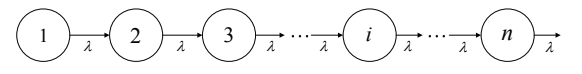
\includegraphics[width=3in]{chapters/chapter3/figures/Figura1-4:DiagramadetransiciondeestadosdeunprocesodePoisson.png}
\caption[Diagrama de transición de estados de un proceso de Poisson]{Diagrama de transición de estados de un proceso de Poisson}
\label{fig:mesh4}
\end{figure}

Para este sistema, el diagrama de transición de estados se presenta en la Figura \ref{fig:mesh4} 1—4, en él los
círculos representan los estados del sistema (número de llegadas o nacimientos) y $ \lambda $ representa la
razón (clientes por unidad de tiempo) asociada con cada transición. Adicionalmente, se necesita la condición de frontera, es decir la probabilidad para el estado $ n = 0 $, cuya expresión se muestra en la ecuación \ref{eqn:1.9}
\\
\begin{equation}
    P_{0}\left ( t+ \Delta t \right )=P_{0}\left ( t \right )P_{0,0}\left ( \Delta t \right )
    \label{eqn:1.9}
\end{equation}
\\
Las expresiones \ref{eqn:1.8} y \ref{eqn:1.9} son suficientes para determinar completamente $ P_{n} \left ( t \right ) $. Al sustituir las probabilidades de las expresiones \ref{eqn:1.3}, \ref{eqn:1.4} y \ref{eqn:1.5} en las ecuaciones \ref{eqn:1.8} y \ref{eqn:1.9} se obtiene \ref{eqn:1.10}.

\begin{equation}
    P_{n}\left ( t+\Delta t \right )=P_{n}\left ( t \right )\left ( 1-\lambda \Delta t \right )+P_{n-1}\left ( t \right )\left ( \lambda \Delta t \right )
    \label{eqn:1.10}
\end{equation}
\\
A partir de \ref{eqn:1.10} y aplicando algunas operaciones elementales y reorganizando se llega a \ref{eqn:1.11}.

\begin{equation}
    \frac{P_{n}\left ( t+\Delta t \right ) - P_{n}\left ( t \right ) }{\Delta t}=-\lambda P_{n}\left ( t \right )+\lambda P_{n-1}\left ( t \right )    
    \label{eqn:1.11}
\end{equation}
\\
Y de forma similar a partir de \ref{eqn:1.9} se llega a \ref{eqn:1.12} 

\begin{equation}
    \frac{P_{0}\left ( t+\Delta t \right ) - P_{0}\left ( t \right ) }{\Delta t}=-\lambda P_{0}\left ( t \right )
    \label{eqn:1.12}
\end{equation}
\\
Al tomar el límite cuando, en \ref{eqn:1.11} y \ref{eqn:1.12}, $ \Delta t \rightarrow 0 $ , este conjunto de ecuaciones se obtiene \ref{eqn:1.13}. En ella $ n\geq 1 $, y se desea, naturalmente, encontrar la solución a estas ecuaciones diferenciales,$ P_{n}\left ( t \right ) $.

\begin{equation}
    \frac{d P_{n}\left ( t \right )}{dt} = -\lambda P_{n}\left ( t \right )+\lambda P_{n-1}\left ( t \right )
    \label{eqn:1.13}
\end{equation}
\\
y 

\begin{equation}
    \frac{dP_{0}\left ( t \right )}{dt} = -\lambda P_{0}\left ( t \right )
    \label{eqn:1.14}
\end{equation}
\\
De la ecuación \ref{eqn:1.14}, es trivial, observar que su solución es \ref{eqn:1.15}

\begin{equation}
    P_{0}\left ( t \right )=e^{-\lambda t}
    \label{eqn:1.15}
\end{equation}
\\
Para $ n = 1 $ se parte de la ecuación \ref{eqn:1.13} en la cual se reemplaza el resultado \ref{eqn:1.15} con lo cual se llega a la ecuación diferencial \ref{eqn:1.16}.

\begin{equation}
    \frac{dP_{1}\left ( t \right )}{dt} = -\lambda P_{1}\left ( t \right )+\lambda e^{-\lambda t}
    \label{eqn:1.16}
\end{equation}
\\
La solución de la ecuación diferencial \ref{eqn:1.16} esta dada en \ref{eqn:1.17}.

\begin{equation}
    P_{1}\left ( t \right )=\lambda te^{-\lambda t}
    \label{eqn:1.17}
\end{equation}
\\
De forma similar la siguiente ecuación diferencial, con $ n = 2 $, es \ref{eqn:1.18}.

\begin{equation}
    \frac{dP_{2}\left ( t \right )}{dt} = - \lambda P_{2}\left ( t \right ) + \lambda^{2}te^{-\lambda t}
    \label{eqn:1.18}
\end{equation}
\\
Por su parte, la solución de \ref{eqn:1.18} es \ref{eqn:1.19}.

\begin{equation}
    P_{2}\left ( t \right )=\frac{\Delta ^{2}t^{2} }{2} e^{-\lambda t}
    \label{eqn:1.19}
\end{equation}
\\
Continuando con un proceso idéntico, se puede encontrar por inducción matemática que la solución general de la ecuación diferencial dada en \ref{eqn:1.13} es la función \ref{eqn:1.20}.

\begin{equation}
    P_{n}\left ( t \right )=\frac{ \left ( \lambda t  \right )^{n} }{n!} e^{-\lambda t}
    \label{eqn:1.20}
\end{equation}
\\
Esta es, como puede notarse por simple inspección, que \ref{eqn:1.20} es la  {\em distribución de Poisson}. En este caso modela la probabilidad de $n$ llegadas (nacimientos) en un intervalo de $n$ segundos para un proceso de Poisson de parámetro $ \lambda $.
\\
\textbf{Ejemplo 1—2: Proceso de Poisson.}
\\
Una central telefónica recibe en promedio 100 llamadas por minuto, de acuerdo con un proceso de Poisson. ¿Cuál es la probabilidad de que no entren llamadas en un intervalo de 5 segundos?
\\\\
La solución es simple. $P_{0}\left ( \frac{1}{12} \right )=e^{-\lambda t}=e^{100*\frac{1}{12}}=0.00024$

\subsection{Media y varianza de un proceso de Poisson.}
Ahora se hará la deducción de la media Ahora se hará la deducción de la $media$ $\mu _{t}$ y la varianza $\sigma _{t}^{2}$ de una distribución de $Poisson.$
Sea $\mu _{t}$ el número medio de llegadas en un intervalo de longitud $t$. De esta manera los cálculos presentados en \ref{eqn:1.21} son los primeros pasos para obtener el resultado. La primera igualdad corresponde a la definición, en la segunda se emplea la expresión \ref{eqn:1.20} mientras que en la tercera y última serie de igualdades se factorizan aquellos elementos que no dependen del índice de la sumatoria.

\begin{equation}
    \mu_{t}=E\left [ N_{t} \right ]=\sum_{n=0}^{\infty}n\left [ \frac{\left ( \lambda t \right )^{n}}{n!}e^{-\lambda t} \right ]=e^{-\lambda t}\sum_{n=1}^{\infty}n\frac{\left ( \lambda t \right )^{n}}{\left ( n-1 \right )!}
    \label{eqn:1.21}
\end{equation}
\\
La deducción continúa en \ref{eqn:1.22} con un cambio de variable muy simple, $ m = n-1 $, y luego, nuevamente, factorizando elementos que no son funcionalmente dependientes del índice de la sumatoria y, finalmente, recordando la expansión en series de Taylor de la función exponencial.

\begin{equation}
    \mu_{t}= e^{-\lambda t}\sum_{m=0}^{\infty}n\frac{\left ( \lambda t \right )^{m+1}}{m!}=e^{-\lambda t} \lambda t \sum_{m=0}^{\infty}n\frac{\left ( \lambda t \right )^{m}}{m!}=e^{-\lambda t}\lambda t\left ( e^{\lambda t} \right )=\lambda t
    \label{eqn:1.22}
\end{equation}
\\
La ecuación $ \mu_{t}=\lambda t $ es un resultado muy intuitivo y, por la misma razón, muy bella. Ella indica que el número medio $ \mu _{t} $ es proporcional a la longitud del intervalo $ t $ y a la razón de llegadas de clientes por unidad de tiempo $ \lambda $. Por su parte, para la varianza $\sigma _{t}^{2}$ , el tratamiento adoptado en este texto es similar al presentado en \cite{kleinrock1975}. Sin embargo, antes de entrar de lleno en su deducción, es útil calcular la siguiente esperanza matemática que aplica para un proceso de Poisson. 

\begin{equation}
    E\left [ N_{t}\left ( N_{t}-1 \right ) \right ]=\sum_{n=0}^{\infty}n\left ( n-1 \right )\frac{\left ( \lambda t \right )^{n}}{n!}e-\lambda t = \sum_{n=2}^{\infty}\frac{\left ( \lambda t \right )^{n}}{\left ( n-2 \right )!}e^{- \lambda t}
    \label{eqn:1.23}
\end{equation}
\\
Ahora, haciendo el cambio de variable $ m=n-2 $ y luego recordando la expansión en series de Taylor para la función exponencial se obtiene \ref{eqn:1.24}.

\begin{equation}
    E\left [ N_{t}\left ( N_{t}-1 \right ) \right ]=e^{- \lambda t}\left ( \lambda t \right )^{2} \sum_{m=0}^{\infty}\frac{\left ( \lambda t \right )^{m}}{m!}=\left ( \lambda t \right )^{2}
    \label{eqn:1.24}
\end{equation}
\\
Con este resultado es fácil deducir la variabilidad en un proceso de Poisson. En primer lugar, la identidad de la varianza \ref{eqn:1.25} brinda un camino.

\begin{equation}
    \sigma _{t}^{2}=E\left [ N_{t}^{2} \right ]-\mu _{t}^{2}
    \label{eqn:1.25}
\end{equation}
\\
Obsérvese que basta con calcular $ E\left [ N_{t}^{2} \right ] $ puesto que $ \mu _{t}^{2}=\left ( \lambda t \right )^{2}  $ como consecuencia de \ref{eqn:1.22}.
Ahora bien, este dato faltante puede encontrarse como se indica en \ref{eqn:1.26}. Ahí se aplican los resultados obtenidos en \ref{eqn:1.22} y \ref{eqn:1.24}.

\begin{equation}
    E\left [ N_{t}^{2} \right ]=E\left [ N_{t} \right ]+E\left [ N_{t} \left (  N_{t}-1 \right )\right ]=\left ( \lambda t \right )^{2}+\lambda t 
    \label{eqn:1.26}
\end{equation}
\\
Sustituyendo \ref{eqn:1.26} y \ref{eqn:1.22} en \ref{eqn:1.25} se concluye \ref{eqn:1.27}, es decir la varianza del proceso.

\begin{equation}
    \sigma _{n}^{2}=\left ( \lambda t \right )^{2}+\lambda t-\left ( \lambda t \right )^{2}=\lambda t
    \label{eqn:1.27}
\end{equation}
\\
En síntesis, el número medio de clientes y su varianza en un proceso de Poisson de nacimientos puros son, respectivamente, $ \mu _{t}=\lambda t $ y $ \sigma _{n}^{2}=\lambda t $.

\subsection{Tiempo entre llegadas.}
El tiempo entre eventos sucesivos en un proceso de llegada (o nacimiento puro) se denomina $tiempo$ $inter$-$llegadas$ o $tiempo$ $entre$ $llegadas$. Para un proceso de Poisson (de nacimiento puro), esos
tiempos son variables aleatorias independientes, distribuidas exponencialmente. Para ver que esto es verdad, sea $T$ el tiempo que trascurre entre dos llegadas sucesivas en un proceso de Poisson, la distribución de $T$ , esto es $F_{r}\left ( t \right )$ ,luego de unos breves pasos, es la expresión dada en \ref{eqn:1.28}.

\begin{equation}
    F_{r}\left ( t \right )=P\left [ T\leq t \right ]=1-P\left [ T>t \right ]=1-P_{0}(t)=1-e^{-\lambda t}
    \label{eqn:1.28}
\end{equation}
\\
Al derivar \ref{eqn:1.28} se encuentra  $f_{r}\left ( t \right )$ , la función de densidad de $T$ ,ésta función se muestra en \ref{eqn:1.29}.
\begin{equation}
    f_{T}\left ( t \right )=\lambda e^{-\lambda t }
    \label{eqn:1.29}
\end{equation}
\\
La expresión \ref{eqn:1.29} es la estructura probabilística del tiempo entre llegadas $T$ y, claramente, pertenece a la $familia$ {\em paramétrica} $exponencial.$

\subsection{Propiedad de pérdida de la memoria.}
La familia exponencial, es la única variable aleatoria continua que tiene la $propiedad$ $de$ {\em pérdida} $de$ $memoria.$ El concepto se puede entender con un ejemplo sencillo. Suponga que un tren llega a una estación de acuerdo con un proceso de Poisson con tiempo medio entre trenes de 20 minutos.
\\\\
Supóngase ahora que un pasajero llegada a la estación y que alguien que está esperando en la plataforma le informa que el último tren llegó hace 19 minutos. ¿Cuál es el tiempo medio que el pasajero que recién llega a la estación de be esperar antes de que el próximo tren llegue?
\\\\
El sentido común (el cual no siempre es un buen consejero) diría que la respuesta natural es un minuto, y esto sería verdad en el caso en el cual la llegada del tren fuera un evento determinístico separado exactamente por veinte minutos. Sin embargo, como se trata de un proceso de llegadas de
Poisson, ¡La respuesta es 20 minutos!
\\\\
Intuitivamente, la explicación de ello es sencilla. Para ver que esto es verdad, es necesario volver atrás con la explicación de lanzamiento de monedas del proceso de Poisson. Una llegada es un evento con resultado positivo (“éxito”) de un “lanzamiento de monedas” en un intervalo infinitamente pequeño. A medida que el tiempo avanza es como un gran número de lanzamientos de monedas. Cuando se pone el proceso de Poisson en este contexto es fácil ver que la distribución hasta el próximo evento positivo, esto es “éxito”, no depende de cuando tiempo ha pasado desde el último evento positivo.
\\\\
Sin embargo, el razonamiento intuitivo no es suficiente. La deducción formal o matemática, es decir, ya no intuitiva, es importante y se encuentra de la siguiente manera. Supóngase que una llegada ocurre en el tiempo $t$=0, se sabe, además de \ref{eqn:1.29}, que la estructura probabilística del
tiempo antes de la siguiente llegada, $T$ , es exponencial. También supóngase ahora que no han ocurrido llegadas antes del tiempo $t_{0}$.
Dada esta información, se desea responder la pregunta ¿cuál
es la distribución del tiempo antes de la siguiente llegada? La respuesta se deduce aquí de forma similar a la expuesta en [1] con la definición de una variable aleatoria ficticia $T^{*}$ y, con ella, deducir su función de distribución $F_{T^{*}}\left ( t \right )$.
\\\\
Por definición de función de distribución $F_{T^{*}}\left ( t \right )=P\left [ T^{*}\leq t \right ]$ e incorporando la información disponible
$F_{T^{*}}\left ( t \right )=P\left [ T^{*}\leq t_{0}+t|T^{*}>t_{0} \right]$. 
\\
Ahora, teniendo en cuenta la definición de probabilidad condicional

$F_{T^{*}}\left ( t \right )=\frac {P\left [ T^{*}\leq t_{0}+t,\wedge ,T^{*}>t_{0} \right ]} {P\left[T^{*}>t_{0}\right ]}=\frac{P\left [ t_{0}<T^{*}\leq t+t_{0} \right ]}{P\left [ T^{*}>t_{0} \right ]}$. De acuerdo con las propiedades de la función de distribución y teniendo en cuenta la expresión \ref{eqn:1.28} 
\\
$F_{T^{*}} \left ( t \right )=\frac {F_{T^{*}}\left ( t+t_{0} \right )-F_{T^{*}}\left ( t_{0} \right )}  {1-F_{T^{*}}\left ( t_{0} \right )}=\frac {\left ( 1-e^{-\lambda \left ( t+t_{0} \right )} \right )-\left ( 1-e^{-\lambda t_{0}} \right )}   {1-\left ( 1-e^{-\lambda t_{0}} \right )}$ de donde se deduce \ref{eqn:1.30}.
\\

\begin{equation}
    F_{T^{*}}\left ( t \right )=1-e^{-\lambda t}
    \label{eqn:1.30}
\end{equation}
\\
Lo que, en palabras sencillas, significa que la estructura probabilística de $T^{*}$ , el tiempo que se debe esperar hasta la siguiente llegada dado que se sabe que ese tiempo $T^{*}$ es más grande que $t^{_{0}}$ , es una variable aleatoria perteneciente a la familia exponencial. Ello implica que $\mu _{T^{*}}=\frac{1}{\lambda }$ y que $\sigma _{T^{*}}^{2}=\frac{1}{\lambda ^{2}}$.
\\\\
Se termina este apartado señalando que la familia paramétrica $discreta$ con la propiedad de pérdida de memoria es la distribución {\em geométrica} razón por la cual se dice que la familia exponencial es al mundo continuo lo que la familia geométrica al mundo discreto. Ambas familias juegan un papel protagónico en los modelos de tráfico en redes de telecomunicaciones.






\subsection{La propiedad de Markov.}
La propiedad de pérdida de memoria se define con mayor precisión como la $propiedad$ $de$ $Markov$. Esta propiedad establece que es posible predecir un estado futuro de un sistema basado (únicamente) en el estado sin necesidad de conocer completamente su historial pasado. En términos de una variable aleatoria real no negativa $ T\in\mathbb{R}^{+}T $, la propiedad de Markov se formaliza, de acuerdo con \cite{kleinrock1975}, en la expresión \ref{eqn:1.31}, para un $t_{0}>0$ dado y específico y para cada $t>0$.

\begin{equation}
    P\left [ T>t_{0}+t|T>t_{0} \right ]=P\left [ T>t \right ]
    \label{eqn:1.31}
\end{equation}
\\
En términos de una variable aleatoria discreta X$\left ( t_{n} \right )$ , la misma propiedad se puede escribir, de acuerdo con [1], como en la expresión \ref{eqn:1.32}. Ahí, los  $t_{i}$ crecen monótonamente y los valores $x_{n}$ pertenecen a un espacio de estados discretos.

\begin{eqnarray}
   P\left [ X\left ( t_{n+1} \right )=x_{n+1}|X\left ( t_{n} \right )=x_{n},\cdots ,X\left ( t_{1} \right )=x_{1} \right ]= \nonumber \\
   P\left [ X\left ( t_{n+1} \right )=x_{n+1}|X\left ( t_{n} \right )=x_{n} \right ]
    \label{eqn:1.32}
\end{eqnarray}
\\
%\begin{eqnarray*}
% \lefteqn{ \sin z = z - \frac{z^3}{3!} +} \\
% & & + \frac{z^5}{5!} - \frac{z^7}{7!} + \cdots
%\end{eqnarray*}
Los sistemas Markovianos son sistemas con pérdida de la memoria. Esto hace que sea “muy simple” su análisis teórico puesto que resulta relativamente fácil describir los cambios de estado del sistema, uno necesita tener en cuenta el tiempo desde la última llegada, o el tiempo que el servicio
ha estado en curso desde el último cliente. Cuando el servicio no es Poisson, lo que significa que no se cuenta con la propiedad de pérdida de la memoria, o el tiempo de servicio no es exponencial entonces no se cuenta con las premisas necesarias para aprovechar ésta virtud. En este caso, el análisis del sistema, incluso en una cola simple, no es un trabajo trivial.
\\\\
Un concepto estrechamente relacionado con la propiedad markoviana es el de $cadena$ $de$ $Markov$. Una cadena de Markov es un proceso (estocástico) de Markov, con un espacio de estados discreto. La Figura 1—4, muestra un diagrama de transición de estados, $DTE$, del sistema de líneas de espera
$(M/M/1)$, en él se ilustra la sencillez que presume garantizar la propiedad de pérdida de la memoria para modelar su comportamiento.



\subsection{Tiempos de servicio exponencial.}
Una conclusión derivada de lo discutido en la sección 1.3.7 es que en un sistema $ \left ( M/M/1 \right ) $
el proceso de llegada, el proceso de llegada, representado por la primera $ M $, es “markoviano” lo que es equivalente a asegurar que (1) el número de clientes que llegan al sistema en un intervalo de tiempo de longitud $ t $ fijo es una variable aleatoria de Poisson, o bien que (2) el tiempo que trascurre entre la llegada del {\em (i-1)-ésimo } y es el {\em i-ésimo } clientes es una variable aleatoria exponencial $ T_{i}\sim Exp\left ( \lambda \right ) $ con independencia entre los $ T_{i} $'s. En consecuencia, se ha reiterado bastante, la estructura probabilística de los tiempos entre llegadas es $ f_{T}\left ( t \right )=\lambda e^{-\lambda t} $ y, por ello, el tiempo medio entre llegadas es $ \mu _{T}=\frac{1}{\lambda} $ mientras que la varianza del tiempo entre llegadas es $ \sigma _{T}^{2}=\frac{1}{\lambda^{2}} $. 
\\
\\
Por otro lado, la segunda $ M $ en un sistema $ \left ( M/M/1 \right ) $ indica que el tiempo $ S_{i} $ que el servidor emplea para atender al {\em i-ésimo } cliente también exhibe la propiedad markoviana; con todo lo que
ello implica. Por ejemplo, implica la propiedad de pérdida de la memoria y la independencia entre los tiempos que el servidor “gasta” atendiendo al cliente $ i $. También implica que los $ S_{i}\sim Exp\left ( \lambda \right ) $. En específico $ f_{S}\left ( s \right )=\mu e^{-\mu s} $ y, por ello, el tiempo medio de atención es $ \mu _{T}=\frac{1}{\mu} $ mientras que la varianza del tiempo de atención es $ \sigma _{S}^{2}=\frac{1}{\mu^{2}} $. En el caso de los tiempos de servicio como variables aleatorias exponenciales $ \mu $ es la tasa de atención (clientes por unidad de tiempo) mientras que $ \frac{1}{\mu} $ es la media del tiempo servicio (unidades de tiempo).
\\
\\
¿Qué tan realista es un tiempo de servicio de naturaleza exponencial? Se ha visto que es razonable como modelo de duración en conversaciones telefónicas. Pero se ha discutido también que tiene algún uso en situaciones donde la base física para su uso es más débil. Por ejemplo, el tiempo que transcurre entre paquetes de información de longitud fija a través de un canal en una red de computadores. A veces este tipo de hipótesis es hecha por conveniencia práctica y elegancia teórica, aunque en gran medida el realismo sea sacrificado.
\\
Con todas sus virtudes y debilidades, la teoría clásica de Teletráfico emplea la familia exponencial porque, de la mano con los procesos de Poisson, los dos conducen a los sistemas de tipo Markovianos que imprimen una elegante y muy loable forma matemática para modelar sistemas complejos de telecomunicaciones.

\subsection{Fundamentos del sistema de colas $(M/M/1)$}
El fundamento probabilístico del modelo del sistema de líneas de espera $(M/M/1)$ se denomina $proceso$ $de$ $nacimiento$ $y$ $muerte$. En él, el estado del sistema $N$ representa en número de clientes dentro del sistema en el instante $t$. Puesto que la dinámica del sistema admite “nacimientos”, es decir llegadas de clientes al sistema y “muertes” es decir salidas de clientes del sistema, el estado no es creciente como sí ocurre tanto en los procesos de “nacimientos puros” o de “muertes puras” conforme aumenta $t$
sino que algunas veces aumentará mientras que en otras disminuirá conforme el tiempo avanza.
\\\\
En el área de computación, redes de computadores y telecomunicaciones hay varios ejemplos de sistemas cuyas dinámicas son, por naturaleza, procesos de nacimiento y muerte. La ejecución de procesos en un sistema multitarea, un enrutador en una red de computadores al cual llegan paquetes
provenientes desde un computador fuente en la búsqueda de su destino final, es decir, otro computador en el sistema de red. El número de nuevas llamadas en una central telefónica, o el número de usuarios conectados en un instante de tiempo particular a un computador con el rol de servidor central. Estos, entre muchos otros campos de aplicación en computación, justifican su 18
estudio matemático para aplicarlo en el diseño y la planeación de sistemas de cómputo, de redes de computadores y de sistemas de telecomunicaciones.
\\\\
El tratamiento formal que se expone a continuación sigue un esquema similar al presentado en \cite{kleinrock1975}. Al ser el proceso de llegadas y el proceso de atención modelos de tipo Markovianos, el Diagrama de Transición de estados, $DTE$, de un proceso de nacimiento y muerte se presenta en la Figura 1—5 \ref{fig:mesh5}.

\begin{figure}[H]
\centering
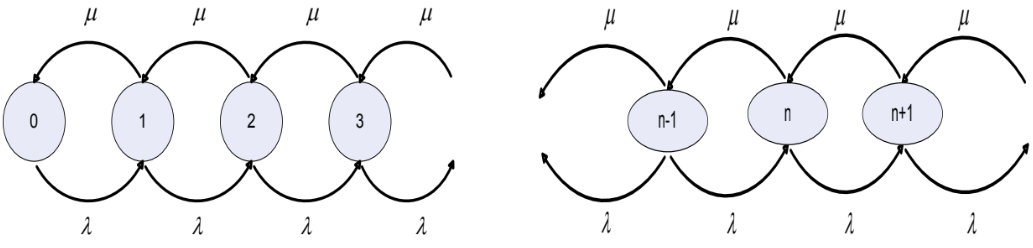
\includegraphics[width=4.5in]{chapters/chapter3/figures/Figura1-5:DiagramadeTransiciondeEstadosDTEdelsistema.png}
%%\centerline{\epsfig{/Chapters/chapter3/figures/Figura1-1:Sistema(mm1).png,width=.8\textheight,height=.4\textwidth}}
\caption[Diagrama de Transición de Estados DTE del sistema (M/M/1)]{Diagrama de Transición de Estados DTE del sistema (M/M/1)}
\label{fig:mesh5}
\end{figure}

De la misma manera como se estudió en la sección 1.3.1, en donde se trataron los sistemas de “nacimiento puro”, se empleará la misma notación para el proceso de nacimiento involucrado aquí. Las expresiones \ref{eqn:1.33}, \ref{eqn:1.34} y \ref{eqn:1.35} son el fundamento del proceso de nacimiento incluido en el proceso general de nacimiento y muerte.


\begin{equation}
   P \left [ Exactamente\; llegada\; en\;\left [ t,t+\Delta t \right ] \right ]=\lambda \Delta t
   \label{eqn:1.33}
\end{equation}



\begin{equation}
    P \left [ Ninguna\; llega\; en\;\left [ t,t+\Delta t \right ] \right ]=1-\lambda \Delta t
    \label{eqn:1.34}
\end{equation}



\begin{equation}
    P \left [ Mas\; de\; 1\; llegada\; en\; \left [ t,t+\Delta t \right ] \right ]=0
    \label{eqn:1.35}
\end{equation}
\\
También es necesario incorporar el proceso (de muerte) de acuerdo con el análisis de la sección 1.3.8. Las expresiones \ref{eqn:1.36}, \ref{eqn:1.37} y \ref{eqn:1.38} son el fundamento del proceso de muerte
incluido en el proceso general de nacimiento y muerte. 

\begin{equation}
   P \left [ Exactamente\; 1\; salida\; en\; \left [ t,t+\Delta t \right ] \right ]=\mu \Delta t
   \label{eqn:1.36}
\end{equation}

\begin{equation}
   P \left [ Ninguna\;  salida\; en\; \left [ t,t+\Delta t \right ] \right ]=1-\mu \Delta t
   \label{eqn:1.37}
\end{equation}

\begin{equation}
   P \left [ Mas\;  de\; 1\; salida\; en\; \left [ t,t+\Delta t \right ] \right ]=0
   \label{eqn:1.38}
\end{equation}
\\
El objetivo es encontrar $P_{n}\left ( t \right )$ , la función de densidad de la variable aleatoria $N_{t}$, es decir el estado del sistema, que denota el número de clientes dentro del sistema en el instante $t$ cuando la dinámica del sistema obedece a un proceso de nacimiento y muerte. Formalmente, la expresión \ref{eqn:1.39} define este concepto.

\begin{equation}
    f_{n_{t}}\left ( n \right )=P_{n}\left ( t \right )\equiv P\left [ N_{t}=n\; en\; el\; intervalo\; [0,t) \right ]
    \label{eqn:1.39}
\end{equation}
\\
Y sea $p_{ij}\left ( \Delta t \right )$ la probabilidad de pasar del estado (número de clientes dentro del sistema) $i$ al estado (número de clientes dentro del sistema) $j$ en un intervalo de tiempo de $\Delta t$ segundos.
\\
A partir de las expresiones numeradas desde la \ref{eqn:1.33} a la \ref{eqn:1.39} se deduce la expresión \ref{eqn:1.40}

\begin{equation}
    P_{n}\left ( t+\Delta t \right )
    = P_{n}\left ( t \right ) p_{n,n}\left ( \Delta t \right )+P_{n-1}\left ( t \right )p_{n-1,n}\left ( \Delta t \right )+P_{n+1}\left ( t \right )p_{n+1,n}\left ( \Delta t \right )
    \label{eqn:1.40}
\end{equation}
\\
Términos de orden superior funcionalmente dependientes de $\Delta t$ son ignorados puesto que son, en magnitud, muy pequeños. La ecuación \ref{eqn:1.40} dice que se puede llegar a tener $n$ clientes en el tiempo
$t+\Delta t$ ya sea porque el estado era $n-1$, $n$ ó $n+1$ clientes en el tiempo $t$. Debido a que se está frente a un proceso de $nacimiento$ $y$ $muerte$, estas son las únicas posibilidades. Para llegar al estado 0, se tendrá la condición inicial y, es evidente que, esa es una situación es especial y que se cumple la ecuación \ref{eqn:1.41}.

 \begin{equation}
     P_{0}(t+\Delta t)=P_{0}(t)p_{0,0}(\Delta t)+P_{1}(t)p_{1,0}(\Delta t)
     \label{eqn:1.41}
 \end{equation}
 \\
 Ahora sustituyendo en la expresión \ref{eqn:1.41} las probabilidades
 $p_{ij}(\Delta t)$ de acuerdo con las definiciones de nacimientos de las ecuaciones \ref{eqn:1.33}, \ref{eqn:1.34} y \ref{eqn:1.35} así como las 
definiciones para el proceso de muertes dadas en las ecuaciones \ref{eqn:1.36}, \ref{eqn:1.37} y \ref{eqn:1.38} para los eventos que ocurren en un intervalo $[t,t+\Delta t]$ , la expresión \ref{eqn:1.40} se convierte en la ecuación

\begin{equation}
    P_{n}(t+\Delta t)=P_{n}(t)(1-\Delta t)(1-\mu \Delta t)+P_{n-1}(t)(\lambda \Delta t)+P_{n+1}(t)(\mu \Delta t)
    \label{eqn:1.42}
\end{equation}
\\
Mientras que, bajo esas mismas consideraciones, la expresión \ref{eqn:1.41} se transforma en \ref{eqn:1.43}.

\begin{equation}
    P_{0}\left ( t+\Delta t \right ) = P_{0}\left ( t \right )\left ( 1-\lambda \Delta t \right )+P_{1}\left ( t \right )\left ( \mu \Delta t \right )
    \label{eqn:1.43}
\end{equation}
\\
Realizando unas sencillas operaciones algebraicas, reorganizando y tomando el límite cuando $ \Delta t \to 0 $ sobre las ecuaciones \ref{eqn:1.42} y \ref{eqn:1.43} se llega a la expresión \ref{eqn:1.44}

\begin{equation}
    \frac{dP_{n}\left ( t \right )}{dt}=-\left ( \lambda+\mu \right )P_{n}\left ( t \right )+\lambda P_{n-1}\left ( t \right )+\mu P_{n+1}\left ( t \right )
    \label{eqn:1.44}
\end{equation}
\\
Y a la ecuación \ref{eqn:1.45}.

\begin{equation}
    \frac{dP_{0}\left ( t \right )}{dt}=-\lambda P_{0}\left ( t \right )+\mu P_{1}\left ( t \right )
    \label{eqn:1.45}
\end{equation}
\\
Para $ n \geq 1 $.
\\


Las ecuaciones diferenciales \ref{eqn:1.44} y \ref{eqn:1.45}, describen la evolución de las probabilidades $P_{n}(t)$ de los estados del sistema de líneas de espera $(M/M/1)$ a través del tiempo. Pero ¿qué significan realmente estas ecuaciones? La respuesta a esta pregunta necesitará una discusión posterior sobre flujos y balances.
\\\\
Un caso muy útil e interesante sucede cuando $\frac{dP_{n}(t)}{dt}=0$; es decir cuando la estructura de probabilidades no cambia en función del tiempo. Esta es la situación que ocurre cuando el sistema de filas ha estado operando por mucho tiempo, el comportamiento se ha estabilizado transitoriamente y en la que el sistema ha llegado a un punto de equilibrio. Por ese motivo se dice que el sistema está en $equilibrio$ o $en$ $estado$ $estable$.
\\\\
En este caso, al ser la derivada igual a cero, las probabilidades asociadas con el estado del sistema no cambiarán (serán constantes) y, en consecuencia, no dependerán del tiempo $t$. Por esa razón no
es necesario escribirlas como funcione $P_{n}\left ( t \right )$ sino como constantes $ p_{n} $. De esta manera, las
ecuaciones diferenciales \ref{eqn:1.44} y \ref{eqn:1.45} se convierten en las expresiones \ref{eqn:1.46} y \ref{eqn:1.47}
respectivamente.

\begin{equation}
    0 = - \left ( \lambda + \mu \right )p_{n}+ \lambda p_{n-1} + \mu p_{n+1}
    \label{eqn:1.46}
\end{equation}

\begin{equation}
    0 = - \lambda p_{0}+\mu p_{1}
    \label{eqn:1.47}
\end{equation}
Para $ n \geq 1 $.
\\

Las ecuaciones resultantes son un conjunto de ecuaciones lineales en lugar de un conjunto de ecuaciones diferenciales, lo cual simplifica su solución. Para calcular las probabilidades de equilibrio, $p_{n} n=0,1,2,\cdots,N$, que gobiernan los estados de cualquier sistema de filas con un número $N$1 finito de estados, se procede de la siguiente manera. Para cada uno de los $N$1 estados se escribe una ecuación global de balance. Esto da un sistema de $N$+1 ecuaciones lineales con $N$+1 incógnitas. Ninguna de estas ecuaciones es redundante y, adicionalmente, debe ser incluida la ecuación \ref{eqn:1.48} para normalizar la solución y, al mismo tiempo, garantizar que el conjunto de todas las probabilidades encontradas constituyan una densidad de probabilidad.

\begin{equation}
    p_{0}+p_{1}+p_{2}+ \cdots + p_{N}=1 
    \label{eqn:1.48}
\end{equation}
\\
La solución del conjunto de ecuaciones lineales puede ser solucionado utilizando técnicas numéricas estándar. La razón por la cual es indispensable obtener todas las probabilidades a partir de ellas (y no antes) es posible determinar las medidas de desempeño, descritas en la sección 1.2.2, para cualquier sistema de líneas de espera.
\\

La dificultad que tiene esta aproximación es que en los modelos de colas reales frecuentemente el número de posibles estados del sistema es extremadamente grande haciendo la solución computacional casi imposible. Por suerte, en esos casos se puede suponer un sistema con capacidad infinita (en la práctica número de estados muy grande) y aplicar para esa situación un resultado matemático de extrema utilidad y belleza. Supóngase que se redibuja el diagrama de Transición de Estados, $DTE$ , del sistema $ \left ( M/M/1 \right ) $ como en la Figura \ref{fig:mesh6}.


\begin{figure}[H]
\centering
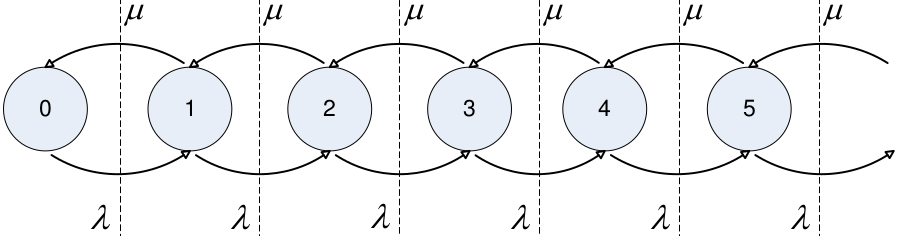
\includegraphics[width=4.5in]{chapters/chapter3/figures/Figura1-6:Balancelocalenlafronteraentreestados.png}
%%\centerline{\epsfig{/Chapters/chapter3/figures/Figura1-1:Sistema(mm1).png,width=.8\textheight,height=.4\textwidth}}
\caption[Balance local en la frontera entre estados]{Balance local en la frontera entre estados}
\label{fig:mesh6}
\end{figure}    

En ese $DTE$ se marcan con líneas punteadas verticales las fronteras entre cada par adyacente de estados. Cada frontera separa el diagrama de estado de transición en dos mitades. Es posible
equiparar el flujo de izquierda a derecha a través de tal frontera con el flujo de derecha a izquierda. Así se obtiene un conjunto de {\em ecuaciones locales de balance}. De cada una de esas fronteras
imaginarias surge una ecuación cuyo patrón se presenta en la expresión \ref{eqn:1.49}.

\begin{equation}
    \lambda p_{n-1}=\mu p_{n}
    \label{eqn:1.49}
\end{equation}
\\
Para $ n=1,2,3,\cdots $ (hasta infinito puesto que se empezó suponiendo un sistema con infinitos estados). Y, de ahí, fácilmente se deduce la ecuación \ref{eqn:1.50}.

\begin{equation}
    p_{n}=\frac{\lambda}{\mu}p_{n-1}
    \label{eqn:1.50}
\end{equation}
\\
Ahora, a través de un sencillo procedimiento recursivo, que se detiene para $ n=1 $, es fácil verificar que la solución de la ecuación en diferencias \ref{eqn:1.50} es \ref{eqn:1.51}.

\begin{equation}
    p_{n}\left ( \frac{\lambda}{\mu} \right )^{2}p_{0}
    \label{eqn:1.51}
\end{equation}
\\
Finalmente, puesto que $ \displaystyle\sum_{n=0}^{+\infty }p_{n}=\sum_{n=0}^{+\infty }\left ( \frac{\lambda}{\mu} \right )^{n}p_{0}=1 $, por ser una función de densidad de probabilidad discreta, se obtiene la probabilidad de que el sistema esté desocupado \ref{eqn:1.52}.

\begin{equation}
    p_{0}=\frac{1}{\displaystyle\sum_{n=0}^{+\infty }\left ( \frac{\lambda}{\mu} \right )^{n}}
    \label{eqn:1.52}
\end{equation}
\\
\section{EL SISTEMA DE FILAS \textit{(M/M/1)} EN DETALLE}
\subsection{Función de densidad}
Es posible simplificar la expresión \ref{eqn:1.52} para calcular p 0 al emplear la “serie geométrica” dada en la identidad \ref{eqn:1.53} con $ \rho = \frac{\lambda}{\mu} $. Para que esa identidad pueda ser empleada es necesario imponer la restricción $ \lambda < \mu $.

\begin{equation}
    \sum_{n=0}^{\infty }\rho=\frac{1}{1-\rho} \; con\;\; 0\leq \rho< 1
    \label{eqn:1.53}
\end{equation}
\\
De esta manera, entonces,$ p_{0}= \left ( 1-\rho \right ) $ y, en consecuencia, la función de densidad sobre los estados del sistema se obtiene a partir de \ref{eqn:1.51} y se presenta en la ecuación \ref{eqn:1.54}.

\begin{equation}
    p_{n}=\left ( 1-\rho \right )\rho_{n}
    \label{eqn:1.54}
\end{equation}
\\
\subsection{Utilización del servidor}
La probabilidad de que el servidor esté ocupado (es decir que no esté libre) se denomina “la utilización del servidor”. Esta probabilidad se interpreta como el porcentaje del tiempo de operación del sistema en el cual el servidor estuvo ocupado atendiendo a los clientes del sistema. Formalmente esta medida de desempeño se calcula como se muestra en la ecuación \ref{eqn:1.55}.

\begin{equation}
    U=P\left [ N_{t}> 0 \right ]=1-P\left [ N_{t}=0 \right ]=1-p_{0}=\rho
    \label{eqn:1.55}
\end{equation}
\\
En consecuencia el parámetro $ \rho = \frac{\lambda}{\mu} $ se conoce como {\em utilización}. La magnitud $ \rho $ puede verse como la \textbf{\textit{carga ofrecida}} normalizada. Esto es, $ \lambda $ puede variar desde cero (carga suave), hasta un valor ligeramente menor que $ \mu $ (carga pesada). Además, $ \rho $ puede variar entre 0 y 1. \\


Aunque para llegar a esta conclusión se supuso que la capacidad del sistema es infinito, en la práctica, sin embargo, las probabilidades de que en el sistema hayan muchos clientes esperando a ser atendidos es relativamente pequeña y depende, obviamente, de la “carga ofrecida” por el sistema.

\subsection{Número medio de clientes en el sistema}
El número medio $ \mu_{N_{t}} $ de clientes que se encuentran en el sistema está dado en la ecuación \ref{eqn:1.56}.
\begin{equation}
    \mu_{N_{t}}=E\left [ N_{t} \right ]=\frac{\rho}{1-\rho}
    \label{eqn:1.56}
\end{equation}
\\
Para mostrar que \ref{eqn:1.56} es cierta, considérense los dos comentarios que siguen:

\begin{enumerate}
    \item $\displaystyle\sum_{n=0}^{\infty }n\rho^{n}=\rho\sum_{n=1}^{\infty }n\rho^{n-1}=\rho\frac{d}{d\rho}\left ( \frac{1}{1-\rho} \right )=\frac{\rho}{\left ( 1-\rho \right )^{2}} $. Es decir que $ \displaystyle\sum_{n=0}^{\infty }n\rho^{n}=\frac{\rho}{\left ( 1-\rho \right )^{2}} $. Este resultado se empleará en uno de los pasos del numeral 2 que sigue.
    \item $ \mu_{N_{t}}=E\left [ N_{t} \right ]=\displaystyle\sum_{n=0}^{\infty }n\rho_{n}=\sum_{n=0}^{\infty }n\left ( 1-\rho \right )\rho^{n}=\left ( 1-\rho \right )\sum_{n=0}^{\infty }n\rho^{n}= \left ( 1-\rho \right )\left [ \frac{\rho}{\left ( 1-\rho \right )^{2}} \right ]=\frac{\rho}{\left ( 1-\rho \right )} $.
\end{enumerate}

La función descrita por la ecuación ( \ref{eqn:1.56} se presenta en la Figura \ref{fig:mesh7}. Lo que es más notable de esta función es un incremento no lineal asintótico en el número medio de clientes en el sistema conforme $ \rho \to 1 $. También es interesante comentar que esta función se utiliza con frecuencia como una “función de penalización” en optimización de algoritmos en filas largas de espera.

\begin{figure}[H]
\centering
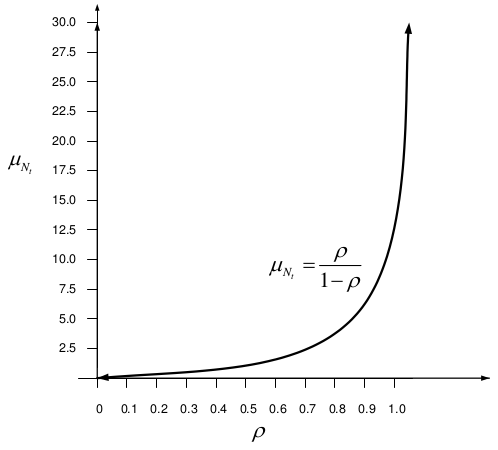
\includegraphics[width=3in]{chapters/chapter3/figures/Figura1-7:Numeromediodeclientesenunsistema.png}
%%\centerline{\epsfig{/Chapters/chapter3/figures/Figura1-1:Sistema(mm1).png,width=.8\textheight,height=.4\textwidth}}
\caption[Número medio de $ \mu_{N_{t}} $ clientes en un sistema (M/M/1)]{Número medio de $ \mu_{N_{t}} $ clientes en un sistema (M/M/1)}
\label{fig:mesh7}
\end{figure}    

\subsection{Varianza del Número de clientes en el sistema.}

LA varianza $ \sigma_{N_{t}}^{2} $ del número de clientes que se encuentran en el sistema está dada en la ecuación \ref{eqn:1.57}. 

\begin{equation}
    \sigma_{N_{t}}^{2}=E\left [ \left ( N_{t}-\mu _{N_{t}} \right )_{t}^{2} \right ]=\frac{\rho}{\left ( 1- \rho \right )^{2}}
    \label{eqn:1.57}
\end{equation}
\\
Para mostrar que \ref{eqn:1.56} es cierta, considérense los dos comentarios que siguen:

\begin{enumerate}
    \item $ \sigma_{N_{t}}^{2}=E\left [ \left ( N_{t}-\mu _{N_{t}} \right )_{t}^{2} \right ]= E\left [ N_{t}^{2} \right ]-\left ( \mu _{N_{t}} \right )^{2} $. Nótese que $ \mu _{N_{t}} $ está dada en la expresión \ref{eqn:1.56} y, por lo tanto, es suficiente con calcular el segundo momento del número de clientes en el sistema $ N_{t} $
    \item Antes de ello es fácil verificar que $ \displaystyle\sum_{n=0}^{\infty }n^{2}\rho^{n}=\frac{\rho \left ( 1+\rho \right )}{\left ( 1-\rho \right )^{3}} $. Este resultado se empleará en uno de los pasos del numeral 3 que sigue.
    \item $ E\left [ N_{t}^{2} \right ] = \displaystyle\sum_{n=0}^{\infty }n^{2}\rho_{n}= \sum_{n=0}^{\infty }n^{2}\left ( 1- \rho \right )\rho^{n}= \left ( 1- \rho \right )\frac{\rho \left ( 1+\rho \right )}{\left ( 1-\rho \right )^{3}}=\frac{\rho \left ( 1+\rho \right )}{\left ( 1-\rho \right )^{2}} $. Finalmente, reemplazando este resultado en el comentario 1, se sigue el resultado. 
\end{enumerate}

El comportamiento de la variabilidad del número de clientes en el sistema se presenta en la Figura
\ref{fig:mesh8}. Al igual que con el número

\begin{figure}[H]
\centering
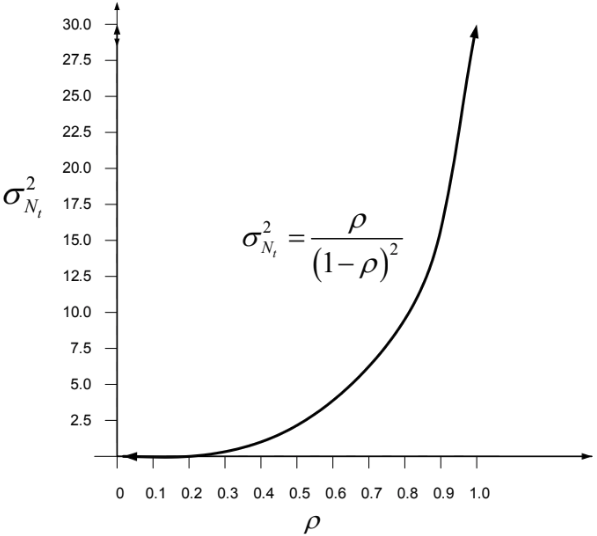
\includegraphics[width=3in]{chapters/chapter3/figures/Figura1-8:Varianzadelnumerodeclientesenunsistema.png}
%%\centerline{\epsfig{/Chapters/chapter3/figures/Figura1-1:Sistema(mm1).png,width=.8\textheight,height=.4\textwidth}}
\caption[Varianza del número de clientes $ \sigma_{N_{t}}^{2} $ en un sistema (M/M/1)]{Varianza del número de clientes $ \sigma_{N_{t}}^{2} $ en un sistema (M/M/1)}
\label{fig:mesh8}
\end{figure} 

\section{LEY DE LITTLE}
La ley de Little es el resultado teórico que permite calcular otra medida de desempeño importante en sistemas de línea de espera: {\em El Tiempo medio que un cliente permanece dentro del sistema. } Formalmente, sea $ T $ la variable aleatoria que representa el tiempo que un cliente “gasta” desde el momento de su llegada al sistema hasta el momento en el cual el servidor termina de atenderlo. De
acuerdo con lo discutido en la sección 1.2.2, entonces, se desea encontrar $ \mu_{T} = E \left[ T \right] $. Una forma de encontrar ésta constante es realizar el cálculo aplicando directamente la definición de esperanza matemática; sin embargo, para ello es necesario contar con $ f_{T}\left( t \right) $, información con la cual no se cuenta.
\\
Una forma alternativa, más directa, simple, eficiente y elegante, es emplear la ecuación llamada la “Ley de Little” \footnote{La notación original empleada por Little para esta ley es $ L=\lambda W. $}

\begin{equation}
    \mu_{N} = \lambda \mu_{T}
    \label{eqn:1.58}
\end{equation}
\\
Nótese que $ \lambda $ es la tasa de llegadas de clientes al sistema de líneas de espera. Así mismo, se cuenta $ \mu_{N_{t}} $ al aplicar la ecuación \ref{eqn:1.56}, en consecuencia, $ \mu_{T} $ se puede deducir fácilmente a partir de \ref{eqn:1.58}.

En \cite{kleinrock1975} se presentan al menos cinco demostraciones diferentes de este interesante y útil resultado\footnote{La ley de Little también se tiene si consideramos la fila y no el servidor, 
esto es $ \mu_{N}^{\left ( Q \right )}=\lambda \mu_{T}^{\left ( Q \right )}. $}. El esquema de demostración que aquí se presenta está inspirado en una de esas pruebas. La Figura\ref{fig:mesh9} ayuda a entender ésta estrategia de demostración.

\begin{figure}[H]
\centering
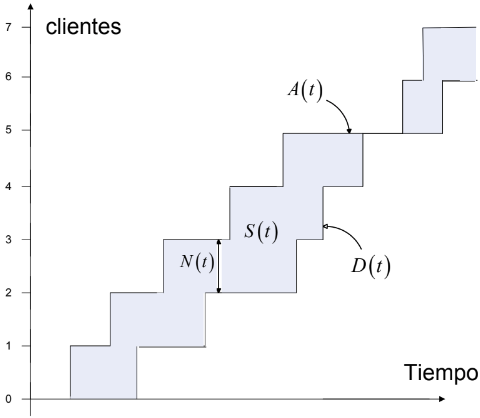
\includegraphics[width=2.5in]{chapters/chapter3/figures/Figura1-9:EsquemadedemostraciondelaLeydeLittle.png}
%%\centerline{\epsfig{/Chapters/chapter3/figures/Figura1-1:Sistema(mm1).png,width=.8\textheight,height=.4\textwidth}}
\caption[Esquema de demostración de la ``Ley de Little'']{Esquema de demostración de la ``Ley de Little''}
\label{fig:mesh9}
\end{figure} 

Las bases de la prueba se enumeran a continuación:

\begin{enumerate}
    \item Considerando el intervalo de tiempo $ \left [ 0,t \right] $ y sean las funciones: $ A \left ( t \right) $ que denota el número de llegadas al sistema hasta el instante $ t $. $ D\left ( t \right) $ que representa el número de salidas del sistema hasta el instante $ t $. Por esta razón $ N\left ( t \right) = A\left ( t \right)-D\left ( t \right) $ será el número de clientes en el sistema en el instante $ t $. 
    \item $ S\left ( t \right) $ es el área acumulada entre las curvas $ A\left ( t \right) $ y $ D\left ( t \right) $ hasta el tiempo $ t $. Esta área es el tiempo total utilizado por todos los clientes que han estado en el sistema hasta el instante $ t $. 
    \item Con ello, ahora, se formalizan tres relaciones evidentes en la Figura \ref{fig:mesh9}.
    \begin{enumerate}
        \item La primera es $ \lambda_{t} = \frac{A\left ( t \right)}{t} $. Aquí, $ \lambda_{t} $ es la tasa media de llegadas durante el $\left [ 0,t \right]$.
        \item La segunda es $ \mu_{T}^{\left ( t \right)} = \frac{S\left ( t \right)}{A\left ( t \right)} $ el tiempo medio que han empleado los cliente en el hasta el instante $ t $.
        \item Y, por último, la tercera ecuación es $ \mu_{N}^{\left ( t \right)} = \frac{S\left ( t \right)}{t} $ el número promedio de clientes hasta el instante $ t $.
    \end{enumerate}
    \item De ahí, es claro que $ \mu_{N}^{\left ( t \right)} = \frac{S\left ( t \right)}{t} = \frac{\mu_{T}^{\left ( t \right)}\times A\left ( t \right) } {t} = \lambda_{t} \times \mu_{T}^{\left ( t \right)} $. Es decir, $ \mu_{N}^{\left ( t \right)} = \lambda_{t} \times \mu_{N}^{\left ( t \right)} $. 
    \item Finalmente, tomando el límite cuando $ t \to \infty $ , $ \mu _{N} =\lim_{t\to 0} \left ( \mu_{N}^{\left( t \right) } \right ) $, $ \lambda \lim_{t\to 0} \left( \lambda_{t} \right)$ y $ \mu _{T} =\lim_{t\to 0} \left ( \mu_{T}^{\left( t \right) } \right ) $, De donde se concluye la ley $ \mu_{N}= \lambda \mu_{T} $.
\end{enumerate}

La ley de Little aplica, en general, para cualquier sistema de líneas de esperas $ \left ( G/G/m \right ) $ y en particular para los sistemas $ \left ( M/M/1 \right ) $, como se muestra en el ejemplo que sigue.
\\
\\
\textbf{Ejemplo 1—3}
El cálculo de $ \mu _{T} $ para el sistema $ \left ( M/M/1 \right ) $ a partir de la “Ley de Little” mostrada en la ecuación \ref{eqn:1.58}, puede realizarse usando el resultado de la ecuación \ref{eqn:1.56}, por lo tanto $  $



\section{TEOREMA DE BURKE}
\begin{theorem}[Teorema de Burke]\label{1th:Z_m}
El proceso de salida de un proceso para un sistema $ \left( M/M/1 \right) $, en equilibrio, es un proceso de Poisson con parámetro $ \lambda $.
\end{theorem}

\section{RESUMEN Y PANORAMA HISTÓRICO}
En este capítulo se estudió la teoría de colas simple, una de las ramas de la investigación de operaciones. El estudio matemático de las filas que se forman en ciertos sistemas es fundamental para optimizar la operación del sistema. Por esta razón, el principal propósito de esta disciplina es caracterizar dicho sistema desde el punto de vista de su rendimiento. Medidas de desempeño tales
como el tiempo de espera medio en las colas o la utilización del sistema para que éste mantenga su normal operación sin que llegue a colapsar o, al menos, conocer las circunstancias que producirían tal situación.
\\
\\
Su aplicabilidad a las ciencias de la computación, las redes de computadores y las telecomunicaciones es evidente. En este sentido, la teoría es muy útil para modelar procesos tales como la llegada de datos a una cola en ciencias de la computación, la congestión de redes de computadores, redes Ad Hoc, sistemas celulares y, en general, redes de telecomunicaciones. Otras aplicaciones en el contexto de la computación son también evidentes. Por ejemplo, los procesos enviados a un servidor para su ejecución forman colas de espera mientras no son atendidos; la información solicitada, a través de Internet, a un servidor Web puede recibirse con demora debido a la congestión en la red. 
\\
\\
El origen de esta teoría se encuentra en los estudios del matemático, estadístico, e ingeniero danés Agner Krarup Erlang quien nació en el año de 1878 y murió en 1929. A él se le da el apelativo de “Padre de la Ingeniería de Teletráfico” puesto que en 1909, para analizar la congestión del tráfico telefónico con el propósito de satisfacer adecuadamente la demanda estocástica de servicios en el sistema telefónico de Copenhague, empezó por formalizar o matematizar el comportamiento de estos sistemas.


\section{EJERCICIOS}

\begin{enumerate}
    \item Dado el sistema de colas determinístico, tanto en su proceso de llegadas como en el de servicio, $ \left ( \lambda / \mu / 1 \right ) $ con tasas de llegadas y de atención $ \lambda, \mu \in \mathbb{R}^{+} $ respectivamente cuyas unidades son $ \displaystyle paquetes / segundo $ . Deduzca formalmente las siguiente medidas de desempeño (Imponga las restricciones y proponga los supuestos que sean necesarios):
    \begin{enumerate}
        \item Utilización.
        \item Número medio de clientes en fila.
        \item Número medio de clientes en el sistema.
        \item Tiempo medio en fila.
        \item Tiempo medio en el sistema.
    \end{enumerate}
    \item Para un proceso binomial con $ \lambda = 5 clientes/Seg  t=10 seg $ y $ \delta t = 0.1 $, encuentre:
    \begin{enumerate}
        \item La función de densidad.
        \item La función percentil.
        \item La varianza.
        \item La función generadora de momentos.
        \item La probabilidad de que después de los primeros $ 5seg $ no lleguen clientes.
    \end{enumerate}
    \item En la sección 1.3.3 se dedujo el modelo de nacimiento puro. Haciendo un desarrollo similar, formule los fundamentos de un proceso de muerte pura.
    \item * Demuestre que, en el caso continuo, la familia exponencial $ T \sim Exp \left ( \lambda \right ) $ es la ÚNICA familia que exhibe la propiedad de pérdida de la memoria.
    \item Con un procedimiento análogo (esto es similar) al empleado en la sección 1.3.6 para demostrar que la familia exponencial presenta la propiedad de pérdida de la memoria, 
    \begin{enumerate}
        \item Demuestre que, en el caso discreto, la familia Geométrica $ T \sim Geo \left ( p \right ) $ presenta la propiedad de pérdida de la memoria.
        \item * Demuestre que, en el caso discreto, la familia Geométrica $ T \sim Geo \left ( p \right ) $ es la ÚNICA familia que exhibe la propiedad de pérdida de la memoria.
    \end{enumerate}
\end{enumerate}


\part{SIMULACIÓN DE SISTEMAS COMPLEJOS}

\chapter{MODELOS MATEMÁTICOS Y SIMULACIÓN}

%Contadores y formato para numeracion de elementos
\renewcommand{\thefootnote}{\arabic{footnote}}
\renewcommand{\theequation}{\arabic{chapter}-\arabic{equation}}
\renewcommand{\thefigure}{\arabic{chapter}.\arabic{figure}}
\renewcommand{\figurename}{Figura}
\renewcommand{\tablename}{\textbf{Tabla}}
\renewcommand{\thetable}{\textbf{\arabic{chapter}-\arabic{table}}}
\newcounter{definitionN}
\newcounter{exampleN}
\newcounter{tableN}
\newcounter{footN}
\newcounter{algorithmN}
\stepcounter{definitionN}
\stepcounter{exampleN}
\stepcounter{tableN}
\stepcounter{footN}
\stepcounter{algorithmN}
\bibliographystyle{apalike}

%Diana Carolina Guarin Angulo
\newpage
En este capítulo se desarrollan las ideas de \textit{\textbf{Sistema, Modelo}} (matemático) y \textit{\textbf{Solución del modelo}}.

Dentro de estos conceptos se plantea el modelo \textbf{SAO} (\textbf{S}istema, \textbf{A}mbiente, \textbf{O}bservatorio), descrito con más detalles en \cite{trivino2010complexSystems} sobre el cual se estructura el estudio formal de un \textbf{Sistema} (complejo) \textbf{S}.

\section{INTRODUCCIÓN}\label{sec:intro}
\setcounter{equation}{0}

La realidad, en medio de la cual se encuentran las personas y los objetos que posibilitan su supervivencia en un mundo generalmente hostil, es compleja. Que una persona pueda sobrevivir en un entorno complejo es gracias, en parte, a la capacidad de abstracción con la que cuentan los humanos (y en general los seres vivos). La abstracción permite representar internamente la realidad a través de esos factores que son esenciales y suprimir los detalles (seguramente importantes) pero innecesarios en un momento particular. Reducir esa realidad a lo relevante le posibilita a las personas comprender lo importante del entorno y le da la capacidad de adoptar decisiones con relativa \textit{eficiencia} pero eso sí, principalmente, con una alta \textit{eficacia}.\\

En este contexto, se llamará \textbf{\textit{Sistema}} a un trozo de la realidad que tiene algún fin particular, el \textbf{\textit{Ambiente}}, que también es un pedazo de la realidad, brinda las condiciones necesarias (y al menos suficientes) para que, en el caso de que el sistema se encuentre inmerso en él, pueda actuar en la búsqueda del cumplimiento de su objetivo.\\

Los humanos, a través de la \textit{ciencia}, han construido algunos sistemas particulares (que como tales son piezas de la misma \textit{realidad}) cuya finalidad es servir de herramientas que permiten comprender la \textit{naturaleza de la realidad} a través de la acción de sistemas en ciertos entornos pero, en particular, comprender el éxito o el fracaso de un sistema en un ambiente. Para ello evalúan el desempeño del sistema en estudio en medio de un ambiente particular. Cada uno de esos sistemas especializados en medir el comportamiento del sistema actuando en un ambiente se les denomina \textbf{\textit{Observatorio}}.\\

A esa abstracción de la realidad que realizan en su permanente quehacer tanto el sistema como el observatorio se denomina \textbf{\textit{modelo}} (de la realidad) pero nótese que el modelo del sistema no tiene por qué ser el mismo del observatorio ni mucho menos de la misma naturaleza. Con frecuencia, el modelo es de naturaleza matemática, caso en el cual corresponde a un conjunto de ecuaciones. A la determinación de los niveles de las variables que resuelven el sistema de ecuaciones se le conoce como la \textbf{\textit{solución del modelo}} matemático.\\

El propósito de este capítulo es, por lo tanto, estudiar los conceptos de \textbf{\textit{Sistema, modelo}}  y \textbf{\textit{solución del modelo}}  y su rol dentro del campo de los modelos estocásticos en computación.

\section{VARIABLE TRASCENDENTAL: EL ESPACIO-TIEMPO}\label{sec:varTrasc}

\textbf{Definición \arabic{chapter}-\arabic{definitionN}: Naturaleza}\\

\stepcounter{definitionN}
Conjunto de todo lo que \textit{\textbf{existe}}, se rige y se armoniza a través de sus propias leyes. Una armonía entendida como la proporción y correspondencia de los objetos (físicos o abstractos) que componen el todo y que hace que ellos no discuerden o se rechacen principalmente (pero no únicamente) cuando simultáneamente concurren en la consecución de algún fin.\\

El sistema y el modelo general se describen formalmente mediante \textit{\textbf{variables}}, \textit{\textbf{parámetros}} y \textit{\textbf{funciones}} que describen características y representan comportamientos. La naturaleza y, en tal virtud, el ambiente está caracterizada por sus variables de estado denominadas \textit{\textbf{El Tiempo— Espacio}}.\\ 

\textbf{Ejemplo \arabic{chapter}-\arabic{exampleN}: El universo \textfrak{U}}\\

\stepcounter{exampleN}
El universo físico que conocemos conformado por las \textit{galaxias}, las \textit{estrellas}, los \textit{planetas} y todos los \textit{cuerpos celestes} regidos y “armonizados” por un conjunto de leyes, entre ellas la ley de la gravitación universal, que generan un orden o \textit{cosmos} que llamamos \textit{mundo} es, probablemente, el
caso más representativo de \textit{naturaleza}.\\

\textbf{Ejemplo \arabic{chapter}-\arabic{exampleN}: Red de computadores estocástica y dinámica}\\

\stepcounter{exampleN}
El mundo digital generado al interior de un sistema de redes de computadores (dispositivos) conectados a través de canales inalámbricos de forma dinámica y estocástica con el fin de brindar servicios de cómputo mediante abstracciones tales como las de agentes artificiales y comunidades de agentes artificiales que cooperan con el propósito de brindar “servicios” al sistema de red es una obra de ingeniería que cumple con rigor la Definición \arabic{chapter}-1 y, en consecuencia, relativo a la
disciplina de la computación es \textit{naturaleza}.\\

\textbf{Definición \arabic{chapter}-\arabic{definitionN}: Espacio-Tiempo}\\

\stepcounter{definitionN}

El Espacio─Tiempo es un espacio vectorial\footnote[\arabic{footN}]{Matemáticamente un \textit{\textbf{espacio vectorial}} sobre un campo $K$ es un conjunto $T \neq \varnothing$ dotado de dos operaciones para las cuales será cerrado: 1.) Operación interna de Suma \textit{\begin{matrix} $+:$ & $TxT$ &$\to$& $T$ \\ \ & $(t_1,t_2)$ & \to & $+(t_1,t_2)$ \end{matrix}} con las propiedades conmutativa, asociativa, elemento neutro \textbf{$e$} y elemento opuesto \textbf{$-t$}. 2.) Operación externa producto \textit{\begin{matrix} $\bullet:$ & $KxT$ &$\to$& $T$ \\ \ & $(t_1,t_2)$ & \to & $\bullet(t_1,t_2)$ \end{matrix}} con las propiedades asociativa, distributiva del producto con respecto a la suma de vectores y distributiva con respecto de la suma de escalares.} $T \in \mathbb{R}^m$, o equivalentemente $T=(T_1,T_2,...,T_m)$, mediante el cual los \textit{objetos} de la \textit{naturaleza} pueden ser ubicados en las coordenadas $t=(t_1,t_2,...,t_m)$ en un universo particular.\\

\stepcounter{footN}
En la Definición \arabic{chapter}-2 el parámetro \textit{m} representa la dimensión espacio-temporal de la naturaleza. Es frecuente que $m=4$ y que $T_1: tiempo$ como se ilustra en la Figura \arabic{chapter}.1. Es decir, que un objeto o entidad se ubica dentro de ese entorno en cuatro (4) dimensiones. La primera de ellas el tiempo en sentido cronológico y las restantes tres (3) corresponden a la ubicación espacial tal como la conocemos y manejamos en nuestra realidad (\textit{\textbf{altura, anchura, profundidad}}). Sin embargo, a decisión y conveniencia del diseñador del sistema o modelo pueden emplearse más o menos dimensiones.\\

En el caso del universo físico conocido es frecuente (pero no universalmente aceptado) adoptar el espacio métrico euclidiano $(T,d)$ donde $T$ es un espacio vectorial euclidiano (es decir, donde se cumplen los cinco postulados de Euclides) y sobre el cual se asocia la medida de \textit{distancia} entre dos puntos $T^{(1)}, T^{(2)}  \in \mathbb{R}^m $ dada por la expresión \ref{twoPointDist}.\\

\begin{equation}
d(T^{(1)},T^{(2)})=\parallel T^{(1)}-T^{(2)} \parallel = \sqrt{\sum^{m}_{i=1}(t_i^{(1)}-t_i^{(2)})^2}
\label{twoPointDist}
\end{equation}

De acuerdo con la Figura \arabic{chapter}.1 un objeto (por ejemplo un agente artificial) puede ubicarse en un instante cronológico en algún punto del espacio tridimensional. A menos que se diga lo contrario, la variable trascendente Espacio-Tiempo será considerada tetra-dimensional con la interpretación aquí señalada.\\
\begin{figure}[H]
     \begin{center}
         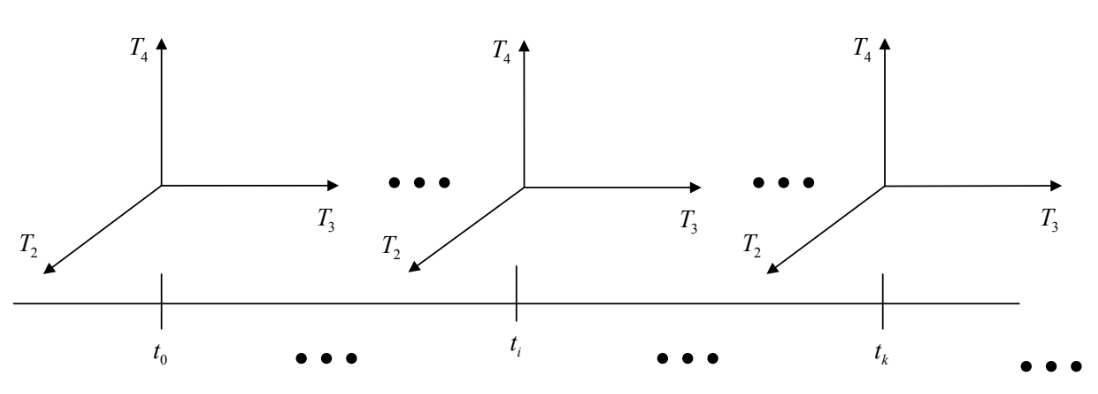
\includegraphics[width=120mm]{chapters/chapter4/figures/espacioTiempo.png}
     \end{center}
     \textbf{\caption{El espacio tiempo tridimensional y tiempo cronológico}}
     \label{fig:1}
\end{figure}

\section{SISTEMA Y AMBIENTE}\label{sec:sistAmbiente}
\textbf{Definición \arabic{chapter}-\arabic{definitionN}: Sistema $\mathbb{S}$}\\

\stepcounter{definitionN}
De acuerdo con \cite{klir2006uncertainityInfoTheory} un sistema $\mathbb{S}$ es un conjunto de entidades o elementos que se interrelacionan entre sí para cumplir uno o más objetivos.\\

\textbf{Ejemplo \arabic{chapter}-\arabic{exampleN}: Pozo Petrolero}\\

\stepcounter{exampleN}

Un pozo petrolero $\mathbb{S}$ es un ingenio humano creado con el fin de poner en contacto un yacimiento de hidrocarburos con la superficie. Dicha conexión entre el yacimiento y la superficie, se realiza con perforaciones de diferentes diámetros llevada a cabo por un taladro capaz de manipular barrenas (usualmente de acero) con rosca en espiral, para la extracción del crudo o gas. Al cumplir la Definición \arabic{chapter}—3, esta obra de ingeniería $\mathbb{S}$ es un sistema.\\

En este caso, los (principales) elementos del sistema son el \textit{hidrocarburo}, el \textit{yacimiento}, el \textit{conjunto de ductos}, los \textit{aparatos} que posibilitan la extracción, las \textit{personas} que operan el pozo, etc. Por otro lado, son claras algunas relaciones que saltan a la vista entre ellos: la relación de “contener” sostenida entre el yacimiento y el crudo, la relación de “extraer” sostenida entre el conjunto de ductos y la maquinaria de extracción, la relación de “operar” presente entre las personas y las máquinas, entre muchas otras relaciones posibles.\\

\textbf{Ejemplo \arabic{chapter}-\arabic{exampleN}: Dispositivo electrónico de suma binaria.}\\

\stepcounter{exampleN}

Un sumador binario en serie es un sistema $\mathbb{S}$ que se puede usar para obtener el resultado de la operación $x+y$. Sean $x=x_5x_4x_3x_2x_1 = 00111$ y $y=y_5y_4y_3y_2y_1 = 01101$ dos números binarios donde $x_1$ y $y_1$ son los bits menos significativos. Los primeros ceros de $x$ y $y$ están ahí para hacer que las cadenas tengan la misma longitud y para garantizar suficientes lugares para completar la suma. La Figura \arabic{chapter}.2 esquematiza esa operación matemática donde $z=z_5z_4z_3z_2z_1 $ es el resultado de la suma y, al igual que con los sumandos, tiene el bit menos significativo en $z_1$.\\

\begin{figure}[H]
     \begin{center}
         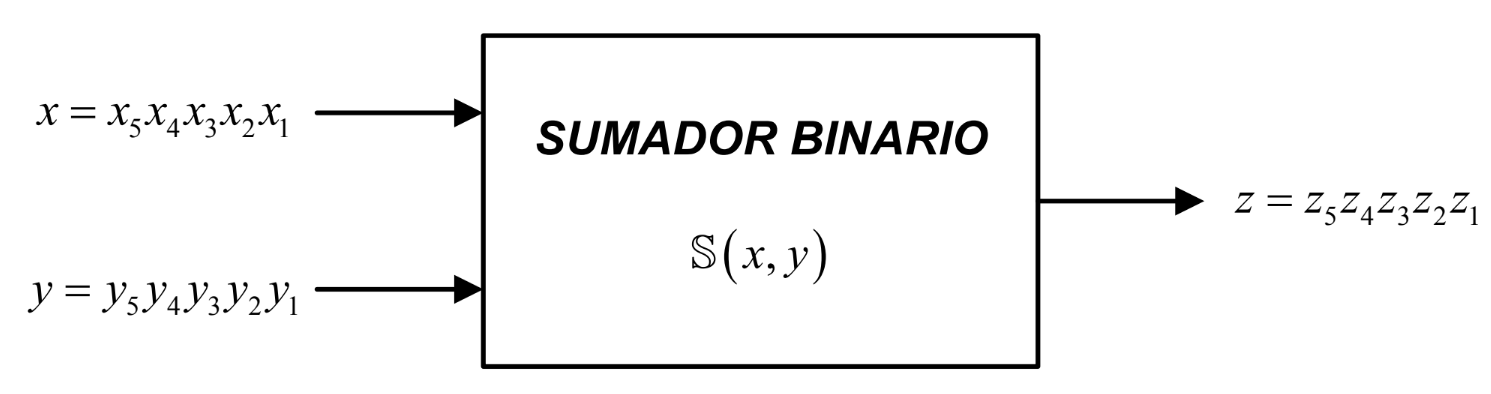
\includegraphics[width=120mm]{chapters/chapter4/figures/sumadorBinario.png}
     \end{center}
     \textbf{\caption{Dispositivo electrónico que suma dos números binarios.}}
\end{figure}

\textbf{Ejemplo \arabic{chapter}-\arabic{exampleN}: Máquina expendedora de chocolatinas.}\\

\stepcounter{exampleN}

Supóngase que en la Facultad de Ingeniería, una máquina $\mathbb{S}$ expendedora de golosinas dispensa dos sabores de chocolatinas: Chocolate negro $(CN)$ y Chocolate blanco $(CB)$. El costo de una unidad de cualquiera de los dos sabores es de $\$200$. La máquina acepta monedas de $ \$50, \$100, \$200 $ y devuelve el cambio necesario.\\

Un día Luis, un estudiante de Modelos estocásticos, decide que le gustaría una Chocolatina negra. Él va a la máquina expendedora, inserta dos monedas de $ \$50 $ y una moneda de $\$100$, en ese orden, y presiona el botón negro, denotado $(BN)$. Paso seguido la máquina le suministra la chocolatina negra. (Para obtener una de chocolatina blanca se presiona el botón blanco, que se denomina $(B)$\\

\begin{table}[h]
\centering
\begin{tabular}{|l|l|l|l|l|l|}
                 & \multicolumn{1}{c|}{$t_0$} & \multicolumn{1}{c|}{$t_1$} &\multicolumn{1}{c|}{$ t_2$} &\multicolumn{1}{c|}{ $t_3$}&\multicolumn{1}{c|}{ $t_4$}\\ 
                 \hline
\textbf{Estado}  & (1) $q_0(\$0)$ & (4) $q_1(\$50)$ & (7) $q_3(\$100)$ & (10) $q_4(\$200)$ & (13) $q_0$ \\ \hline
\textbf{Entrada} & (2) $\$50$ & (5) $\$50$ & (8) $\$100$ & (11) $(BN)$ &  \\ \hline
\textbf{Salida}  & (3) Nada & (6) Nada & (9) Nada & (12) $(CN)$ &  \\ 
\end{tabular}
\caption{\textbf{Secuencia de eventos en la compra de Luis.}}
\label{tab:compraLuis}
\end{table}
\stepcounter{tableN}

El procedimiento seguido por Luis, al hacer su compra, puede representarse como se muestra en la Tabla ~\ref{tab:compraLuis} donde $t_0$ es el tiempo inicial, cuando él inserta su primera moneda, y $t_1$, $t_2$, $t_3$, $t_4$, son momentos posteriores en el tiempo, con $t_1 < t_2 < t_3 < t_4$. Los números $(1),(2),(3),...,(13)$ en esa tabla indican el orden de los \textit{\textbf{eventos}} (para una definición más detallada de este concepto, véase la Definición \arabic{chapter}—12 ) en la compra de la chocolatina negra. Para cada entrada en el tiempo $t_i$, $0\leq i \leq 3$, hay en ese momento una salida correspondiente y luego un cambio de estado. El nuevo estado en el tiempo $t_{i+1}$ depende tanto de la entrada como del estado (presente) en el tiempo $t_i$. La Tabla ~\ref{tab:compraAmigoLuis} muestra la secuencia de eventos en otra compra de chocolatina que realiza un amigo de Luis.\\

\begin{table}[H]
\centering
\begin{tabular}{|l|l|l|l|}
                 & \multicolumn{1}{c|}{$t_0$} & \multicolumn{1}{c|}{$t_1$} &\multicolumn{1}{c|}{$ t_2$} \\ \hline
\textbf{Estado}  & (1) $q_0(\$0)$ & (4) $q_4(\$200)$ & (7) $q_0$   \\ \hline
\textbf{Entrada} & (2) $\$500$ & (5) $(B)$ &    \\ \hline
\textbf{Salida}  & (3) $\$300$ de cambio & (6) $CB$ &   \\ 
\end{tabular}
\caption{\textbf{Secuencia de eventos en la compra del amigo de Luis.}}
\label{tab:compraAmigoLuis}
\end{table}
\stepcounter{tableN}

\textbf{Definición \arabic{chapter}-\arabic{definitionN}: Sistema Complejo \textit{SC}}\\

\stepcounter{definitionN}

El sistema $\mathbb{S}$ se dice complejo \textit{SC} cuando el número de elementos así como el número de interacciones o relaciones entre ellas es significativamente grande \cite{trivino2010complexSystems}.\\

\textbf{Definición \arabic{chapter}-\arabic{definitionN}: Ambiente $\Delta$}\\

\stepcounter{definitionN}

El \textbf{ambiente} $\Delta$ del sistema, también llamado \textit{\textbf{entorno}} o \textit{\textbf{medio ambiente}}, es una porción del universo $\textfrak{U}$, es decir $\Delta \subseteq \textfrak{U} $, que corresponde al conjunto de componentes materiales o inmateriales dentro de los cuales se desenvuelve un sistema $\mathbb{S}$ particular.\\

\textbf{Definición \arabic{chapter}-\arabic{definitionN}: Interfaz de comunicación $\ell$}\\

\stepcounter{definitionN}

Una \textit{\textbf{interfaz}} $\ell$ es un medio físico, perteneciente al universo $\textfrak{U}$, a través de la cual se puede intercambiar algún tipo de señal sobre la cual se puede establecer un lenguaje que permite realizar un \textit{\textbf{dialogo}} o \textit{\textbf{comunicación}} entre el \textit{ambiente} $\Delta$ y un \textit{sistema} $\mathbb{S}$. Normalmente un sistema cuenta con varias interfaces que posibilitan las entradas y las salidas desde el ambiente hacia el sistema y viceversa.\\

\textbf{Ejemplo \arabic{chapter}-\arabic{exampleN}: Medio ambiente biológico}\\

\stepcounter{exampleN}

Considérese el sistema $\mathbb{S}$ : Ser humano. Es decir una persona vista como sistema. En este caso, \textit{el medio ambiente} corresponde a la colección de elementos naturales, sociales y culturales existentes
en una porción del espacio-tiempo $ \tau \subseteq$ $T$ que influyen en la vida de la persona $\mathbb{S}$. Nótese que el medio ambiente no solamente contempla los elementos naturales necesarios para la vida sino que también incluye otros elementos inmateriales tales como los relacionados con la cultura. De otro lado, las interfaces de este sistema $\mathbb{S}$ son los órganos sensoriales u órganos de los sentidos.\\

\textbf{Ejemplo \arabic{chapter}-\arabic{exampleN}: Medio ambiente sociocultural}\\

\stepcounter{exampleN}

Considérese el sistema $\mathbb{S}$ presentado en el Ejemplo \arabic{chapter}—3. Los elementos del conjunto \{\textit{territorio, empresa estatal de petróleos, Instituciones, fauna, flora, ...}\} y sus relaciones constituyen un \textbf{ambiente} $\Delta$ para el \textbf{sistema} $\mathbb{S}$.\\

\section{MODELO DEL SISTEMA}\label{sec:modDelSistema}
\textbf{Definición \arabic{chapter}-\arabic{definitionN}: Modelo del sistema $\textfrak{M}$}\\

\stepcounter{definitionN}

Un modelo $\textfrak{M}$ de un sistema $\mathbb{S}$ es una representación o abstracción del sistema. Sobre ésta abstracción es posible experimentar e inferir comportamientos que, posteriormente, también se pueden asociar al sistema real que es objeto del estudio. Esta asociación es posible gracias al principio de \textit{\textbf{isomorfismo}} (matemático) o bien al concepto de \textit{\textbf{analogía}}. El modelo puede ser una réplica del sistema o bien una abstracción de sus principales características y propiedades.\\

\textbf{Definición \arabic{chapter}-\arabic{definitionN}: Máquina de estados finitos \textit{$M$}}\\

\stepcounter{definitionN}

Una \textbf{\textit{máquina de estados finitos}} $\textit{M}=(\Sigma_e,\Sigma_s,Q,\delta,\varphi)$ donde:
\begin{enumerate}
    \item $\sum_{e}=\left\lbrace a_i \right\rbrace_{i=0}^{i=n_e}$ es el lenguaje de entrada de $\mathbb{S}$,
    \item $\sum_s=\left\lbrace b_j \right\rbrace_{j=0}^{j=n_s}$ es el lenguaje de salida de $\mathbb{S}$,
    \item $Q=\left\lbrace q_r \right\rbrace_{r=0}^{r=n_Q}$ es el conjunto de estados del sistema $\mathbb{S}$,
    \item La \textbf{\textit{función siguiente estado}} $\delta$ dada por:\\
    
    \begin{matrix} $\delta:$ & $\textit{Q} x \sum_e$ &$\to$& $\textit{Q}$ \\ \ & $(q_j,a_i)$ & \to & $q_r$ \end{matrix}
    \item La \textbf{\textit{función respuesta estado}} $\varphi$ dada por:\\
    
    \begin{matrix} $\varphi:$ & $\textit{Q} x \sum_e$ &$\to$& $\sum_s$ \\ \ & $(q_j,a_i)$ & \to & $b_r$ \end{matrix}
\end{enumerate}
Es un modelo matemático $\textfrak{MM}$ para un sistema $\mathbb{S}$.\\

\textbf{Definición \arabic{chapter}-\arabic{definitionN}: Modelo matemático $\textfrak{MM}$ del sistema $\mathbb{S}$}\\

\stepcounter{definitionN}
Un modelo matemático $\textfrak{MM}$ es un tipo particular de modelo $\textfrak{M}$ del sistema $\mathbb{S}$ que representa o abstrae los \textit{\textbf{elementos}}, las \textbf{\textit{relaciones}} entre ellos y los \textit{\textbf{comportamientos}} de $\mathbb{S}$ en función del \textbf{\textit{Espacio-Tiempo}} a través de una (o varias)\footnote[\arabic{footN}]{Para \textit{\textbf{sistemas complejos}}, como se presentará en el siguiente capítulo, se extenderá el concepto de máquina de estado finito a \textit{\textbf{autómata de aprendizaje}} y \textit{\textbf{redes de autómatas adaptativas de aprendizaje}}.} máquinas de estado finitos que siguen la Definición \arabic{chapter}—8.\\

\stepcounter{footN}
\textbf{Definición \arabic{chapter}-\arabic{definitionN}: Modelo matemático $\textfrak{MM}$ del ambiente $\Delta$}\\

\stepcounter{definitionN}

Un modelo matemático $\textfrak{MM}$ es un tipo particular de modelo $\textfrak{M}$ del ambiente $\Delta$ que representa o abstrae la \textbf{\textit{naturaleza}} (véase la Definición \arabic{chapter}—1) y el \textbf{\textit{comportamiento}} de $\Delta$ en función del \textbf{\textit{Espacio-Tiempo}} $\textit{T} \in \mathbb{R}^m$ a través de una (o varias) máquinas de estado finitos que siguen la Definición \arabic{chapter}—8.\\

\textbf{Ejemplo \arabic{chapter}-\arabic{exampleN}: Modelo matemático para la máquina expendedora de chocolatinas}\\
\stepcounter{exampleN}
Para el sistema $\mathbb{S}$ del Ejemplo \arabic{chapter}—5, un modelo matemático $\textfrak{MM}$ se deduce de la Definición \arabic{chapter}—8 la máquina de estados finitos $\textit{M}=(\Sigma_e,\Sigma_s,Q,\delta,\varphi)$ como sigue.\\

\begin{enumerate}
    \item $\sum_{e}=\left\lbrace \$50,\$100,\$200,\textit{B},\textit{N} \right\rbrace$ donde \textit{N} indica el botón negro que se presiona para una chocolatina negra y \textit{B} el botón blanco para una de color blanco.
    \item $\sum_s=\left\lbrace \textit{n},\textit{CB},\textit{CN},\$50,\$100,\$200 \right\rbrace$ \textit{n} : nada, \textit{CN} : Chocolatina negra, \textit{CB} : Chocolatina blanca. 
    \item $Q=\left\lbrace q_0,q_1,q_2,q_3,q_4 \right\rbrace$, donde en el estado $q_k$,para cada $0 \leq k \leq 4$, la maquina recuerda retener $ \$50k $.
\end{enumerate}
Además, las funciones siguiente estado $\delta$ y respuesta $\varphi$ se presentan en el la Tabla ~\ref{tab:funTransicionEstadosDeltaRespuestaPhi} y se representan gráficamente en el DTE de la Figura \arabic{chapter}—3.\\

El estudio de un sistema, con el propósito de entenderlo y, probablemente, intervenirlo de alguna forma, puede realizarse en cualquiera de las formas presentadas en la Figura \arabic{chapter}—4. De la gráfica se infiere que un posible camino es experimentar directamente con el sistema objeto de estudio. Esta vía no es recomendada debido a que la experimentación puede afectar (negativamente) su comportamiento de forma definitiva e irreversible. La segunda ruta es construir un modelo y experimentar sobre el modelo. El modelo puede ser físico (como por ejemplo una maqueta) o matemático (generalmente expresado mediante un conjunto de ecuaciones, frecuentemente ecuaciones diferenciales que describen el comportamiento a lo largo del tiempo de ese sistema).\\


\begin{table}[H]
\centering
\begin{tabular}{|l|l|l|l|l|l|l|l|l|l|l|}

\multirow{}{}{} & \multicolumn{5}{c|}{$\sum_e$}                            & \multicolumn{5}{c|}{$\sum_s$} \\ \cline{2-11} 
        & $\$50$ & $\$100$ & $\$200$ & $BB$ & $BN$ & $\$50$ & $\$100$ & $\$200$ & $BB$ & $BN$ \\ \hline
$q_0$   & $q_1$  & $q_2$ & $q_4$ & $q_0$ & $q_0$ &  $n$  &  $n$  &  $n$  &  $n$  &  $n$ \\ \hline
$q_1$   & $q_2$  & $q_3$ & $q_4$ & $q_1$ & $q_1$ &  $n$  &  $n$  &  $\$50$  &  $n$  &  $n$ \\ \hline
$q_2$   & $q_3$  & $q_4$ & $q_4$ & $q_2$ & $q_2$ &  $n$  &  $n$  &  $\$100$  &  $n$  &  $n$ \\ \hline
$q_3$   & $q_4$  & $q_4$ & $q_4$ & $q_3$ & $q_3$ &  $n$  &  $\$50$  & $\$150$   &   $n$  &   $n$ \\ \hline
$q_4$   & $q_4$  & $q_4$ & $q_4$ & $q_0$ & $q_0$ &  $\$50$  & $\$100$   & $\$200$   &  $CB$ &   $CN$\\ 
\end{tabular}
\caption{\textbf{Funciones de transición de estados $\delta$ y de respuesta $\varphi$ de $M$}}
\label{tab:funTransicionEstadosDeltaRespuestaPhi}
\end{table}
\stepcounter{tableN}

\begin{figure}[H]
     \begin{center}
         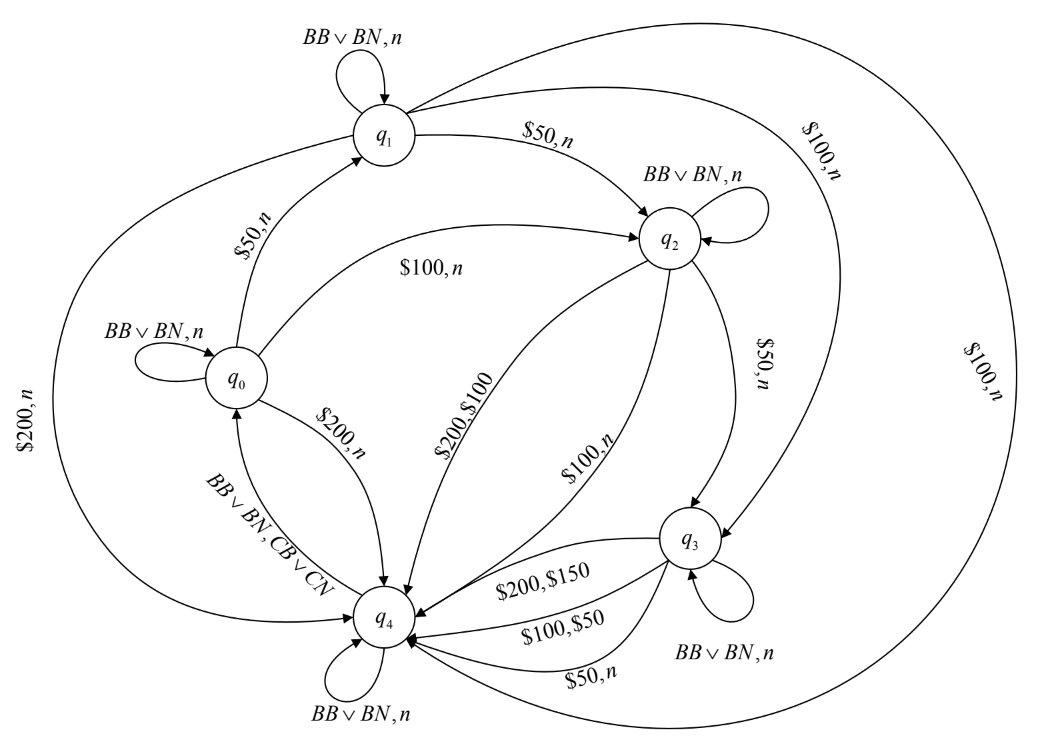
\includegraphics[width=120mm]{chapters/chapter4/figures/DTEmaquinaChocolatinas.png}
     \end{center}
     \textbf{\caption{DTE Para la máquina expendedora de chocolatinas.}}
\end{figure}

Para sistemas simples esta puede ser una tarea relativamente sencilla; sin embargo, cuando el sistema es complejo lo más probable es que su solución de tipo analítico sea imposible calcularla. Por esa razón, la alternativa plausible es encontrar una solución aproximada del modelo mediante técnicas de simulación. Aunque también es posible que sea imposible (principalmente por complejidad computacional), existe una mayor probabilidad de aproximar la solución con un nivel de error máximo permitido. Por este camino no se tiene la solución exacta o analítica pero si se puede encontrar una buena aproximación \cite{law1991simulationModeling}.\\

\section{SOLUCIÓN DEL MODELO MATEMÁTICO}\label{sec:SolModeloMatematico}
\subsection{Tipos de Soluciones}\label{subsec:TiposDeSoldeModMat}
Una vez se tiene el modelo, es necesario solucionarlo. Cuando se trata de un modelo matemático el objetivo es, generalmente, encontrar la solución al sistema de ecuaciones que modelan su comportamiento. De acuerdo con la Figura \arabic{chapter}—4 la solución del modelo matemático $\textfrak{MM}$ puede obtenerse o bien de forma analítica (también conocida como teórica o ideal) o bien a través de experimentación. Una de las formas más frecuentemente empleadas para encontrar la solución del modelo es mediante la técnica heurística llamada simulación.\\

\begin{figure}[H]
     \begin{center}
         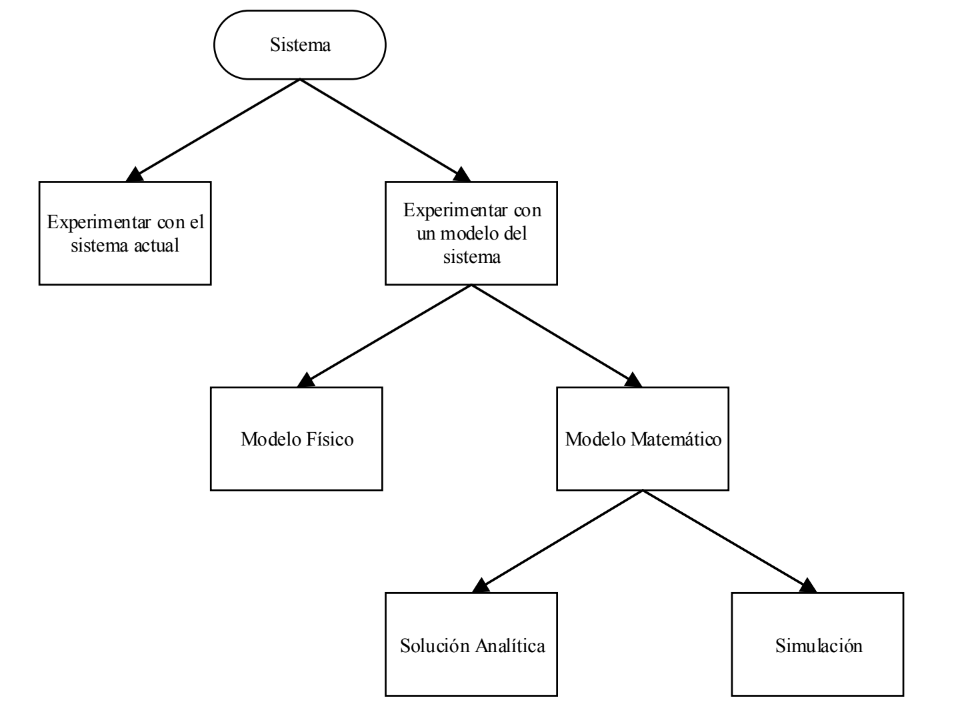
\includegraphics[width=120mm]{chapters/chapter4/figures/formasEstudioSistemaAverrilLaw.png}
     \end{center}
     \textbf{\caption{Posibles formas para estudiar un sistema (Tomada de \cite{law1991simulationModeling}).}}
\end{figure}

La simulación, por su lado, es para R.E. \textbf{Shannon}, \textit{” es el proceso de diseñar un \textbf{modelo} de un \textbf{sistema real} y llevar a término experiencias con él, con la \textbf{finalidad de comprender el comportamiento} del sistema o evaluar nuevas estrategias —dentro de los límites impuestos por un cierto criterio o un conjunto de ellos— para el funcionamiento del sistema”}. \textbf{Simular}, entonces, puede entenderse como sinónimo de \textbf{Imitar} con el fin de conocer el \textbf{comportamiento} del sistema para asumir algunas \textbf{decisiones} que afecten su actividad o estructura.\\

Existen varios paradigmas de simulación, entre los que se destacan tres: El \textbf{\textit{paradigma de dinámica de sistemas}}, el \textbf{\textit{paradigma de simulación de eventos discretos}} y el \textbf{\textit{paradigma de agentes artificiales}}. Una solución experimental del modelo matemático $\textfrak{MM}$ a través de simulación, típicamente, emplea los tres paradigmas antes mencionados.\\

\begin{table}[H]
\centering
\begin{tabular}{|p{2.2cm}|p{1.4cm}|p{1.4cm}|p{1.4cm}|p{0.1cm}|p{1.4cm}|p{1.4cm}|p{1.4cm}|}

                                  & \multicolumn{3}{c|}{\textbf{Ecuaciones Lineales}}                               & \multirow{}{}{} & \multicolumn{3}{c|}{\textbf{Ecuaciones no Lineales}}                            \\ \cline{1-4} \cline{6-8} 
\textbf{Ecuación}                 & \textbf{Una Ecuación} & \textbf{Varias Ecuaciones} & \textbf{Muchas Ecuaciones} &                   & \textbf{Una Ecuación} & \textbf{Varias Ecuaciones} & \textbf{Muchas Ecuaciones} \\ \cline{1-4} \cline{6-8} 
\textbf{Algebraica}               & Trivial               & Fácil                      & Casi Imposible             &                   & Muy Difícil           & Muy Difícil                & Imposible                  \\ \cline{1-4} \cline{6-8} 
\textbf{Diferenciales Ordinarias} & Fácil                 & Difícil                    & Casi                       &                   & Muy Difícil           & Imposible                  & Imposible                  \\ \cline{1-4} \cline{6-8} 
\textbf{Diferenciales Parciales}  & Difícil               & Casi                       & Imposible                  &                   & Imposible             & Imposible                  & Imposible                  \\ 
\end{tabular}
\caption{\textbf{Alcances y limitaciones de los modelos (Tomada de \cite{bertalanffy1968systemTheory}).}}
\label{tab:alcanLimitModelosVonBertalanffy}
\end{table}
\stepcounter{tableN}
\subsection{Limitaciones de los Modelos Matemáticos}\label{subsec:LimitdeModMat}
En este punto resulta interesante recordar los ya clásicos enunciados que se encuentran en \cite{bertalanffy1968systemTheory} y que se resumen en la Tabla ~\ref{tab:alcanLimitModelosVonBertalanffy}. En su disertación describe cómo los modelos matemáticos van desde los muy simples cuyas soluciones son relativamente triviales hasta los muy complejos en los cuales los sistemas de ecuaciones diferenciales parciales del modelo encontrado no tiene solución práctica.\\

En el marco del proyecto de estudio de un sistema complejo \textit{SC} esas conclusiones son importantes si se tiene en cuenta que los modelos matemáticos subyacentes al tipo de sistemas que se intenta comprender pueden tener decenas de ecuaciones diferenciales parciales que describen la dinámica de los estados del sistema en función del \textit{\textbf{espacio -- tiempo}}. En conclusión, las soluciones analíticas para este caso son imposibles de solucionar mediante una forma cerrada encontrada analíticamente.\\

Lo interesante es que a través de aproximaciones basados en estudios de simulación, \cite{law1991simulationModeling} han mostrado que ese tipo de inconvenientes pueden ser ignorados (al menos en parte con estudios serios de simulación).\\

\section{EL MODELO SAO}\label{sec:SAOModel}
De acuerdo con las clases de modelos que se deducen de la Figura \arabic{chapter}—4, SAO es un modelo matemático. Por cada elemento de la sigla existe un módulo: SAO (Sistema, Ambiente y Observatorio). Véase la Figura \arabic{chapter}—5.\\

\subsection{Módulos del Modelo}\label{subsec:ModulosdelModelo}
Aunque el \textit{\textbf{sistema}} es una entidad que puede ser estudiada de forma aislada, la verdad es que todos los sistemas se encuentran inmersos dentro de un \textit{\textbf{entorno}}. Por esa razón, al tiempo que se modela es sistema, es necesario también, incluir dentro del modelo, la representación del ambiente en el cual se desenvuelve ese sistema (puesto que se trata de determinar su comportamiento en ese ambiente particular).\\

\begin{figure}[H]
     \begin{center}
         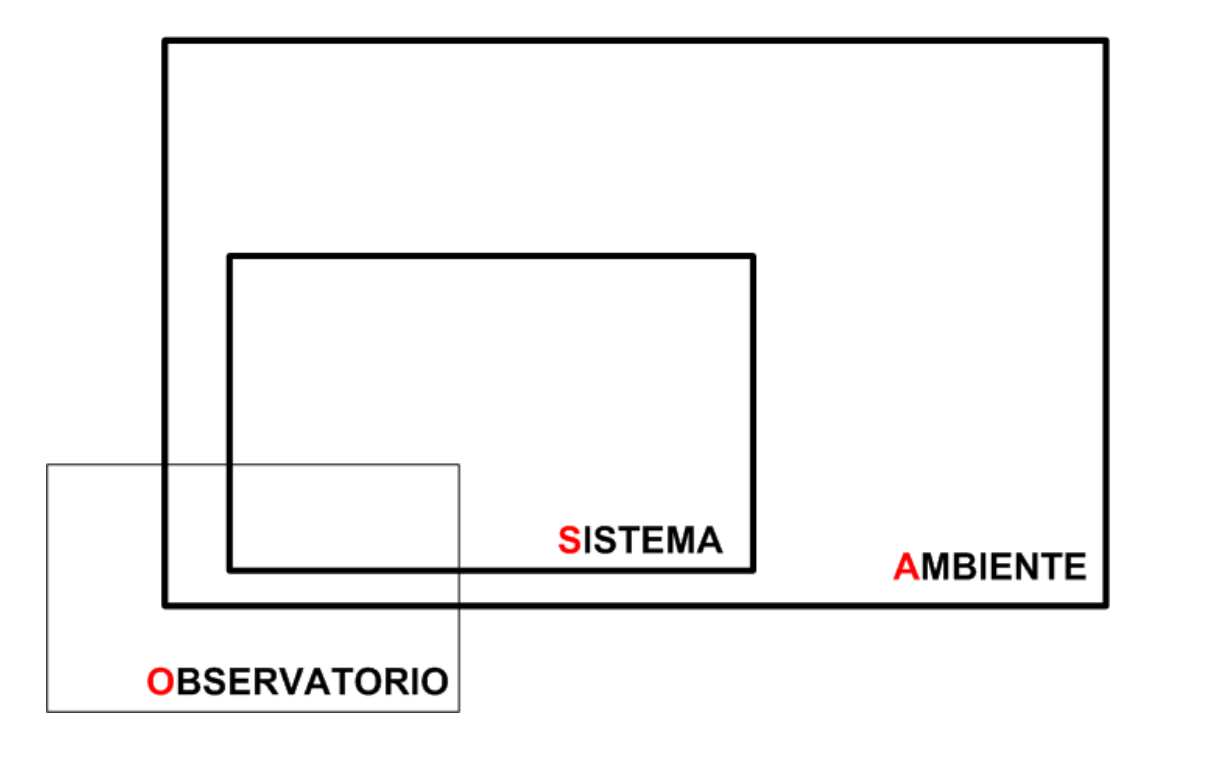
\includegraphics[width=90mm]{chapters/chapter4/figures/modeloSAO.png}
     \end{center}
     \textbf{\caption{Modelo SAO (Adaptado de \cite{trivino2012esthocasticModels})}}
\end{figure}

Con el fin de poder estudiarlo y caracterizarlo, se requiere un elemento más dentro de este esquema. Ese elemento fundamental dentro del propósito de realizar una simulación del sistema, es el \textit{\textbf{observatorio}}. El observatorio, como su nombre lo indica, tiene como finalidad medir o cuantificar u observar el desempeño de ese sistema dentro de ese ambiente. A todos los elemento que deben ser diseñados y, a la larga, simulados se les da el nombre genérico de Modelo SAO que se refiere a Sistema, Ambiente y Observador. Esa arquitectura se presenta de forma gráfica en la Figura \arabic{chapter}—5. Ese esquema es, precisamente, el seleccionado para construir el prototipo del sistema MIA.\\

\subsection{Especificación Matemática}\label{subsec:EspecifMatem}
Un segundo objeto matemático que caracteriza el ambiente es su \textit{\textbf{estado}}. Por ejemplo, en un sistema físico existen propiedades tales como la temperatura, la gravedad, el campo magnético, etc. Este tipo de objetos propios del ambiente se definen formalmente mediante las expresiones ~\ref{estadosConjDeAmbiente}.\\

\begin{equation}
\begin{matrix} $X \in \mathbb{R}^n$ \\ \ $X=(X_1,X_2,...,X_n)$ \end{matrix}
\label{estadosConjDeAmbiente}
\end{equation}

Cada una de las variables que conforman el Estado del sistema es, en sí misma, una función que depende del tiempo y del espacio como se escribe matemáticamente en la expresión ~\ref{estadoDeAmbiente1}.\\
\begin{equation}
\textit{\begin{matrix} $X_i:$ &  \mathbb{R}^m &$\to$&  \mathbb{R} \\ \ & $t$ & \to & $X_i = X_i(t)$ \end{matrix}}
\label{estadoDeAmbiente1}
\end{equation}

En sistemas de alta complejidad el estado del ambiente ~\ref{estadosConjDeAmbiente} es un vector aleatorio, lo cual supone la existencia de una estructura probabilística que lo rige, es decir, una función de densidad de probabilidad conjunta, como se escribe en la expresión ~\ref{funDensidadEstadoAmbiente1}.\\

\begin{equation}
\textit{$f_X(x)=f_{X_1,X_2,...,X_n}(x_1,x_2,...,x_n)$}
\label{funDensidadEstadoAmbiente1}
\end{equation}

Parámetros del Modelo son constantes que no cambiarán su valor durante una corrida de la simulación pero que, con el ánimo de poder realizar análisis de sensibilidad se dejan expresados no como valores específicos sino como letras que los representan. Formalmente se definen como en la expresión ~\ref{funParametros}\\

\begin{equation}
\begin{matrix} $\xi \in \mathbb{R}^q$ \\ \ $\xi=(\xi_1,\xi_2,...,\xi_q)$ \end{matrix}
\label{funParametros}
\end{equation}

Por último, los comportamientos, leyes o características, definidas formalmente mediante la expresión ( \ref{comportamientosEq}), son propiedades de sistemas que pretende con el estudio estimar, encontrar o corroborar. Ellos son la razón de ser de la simulación puesto que son conductas que muchas veces ni siquiera se sabe que existen pero son una realidad la gran mayoría de las veces ocultas. La ley de gravedad en el universo físico es una de ellas. Están ahí y afectan a los objetos que actúan en ese contexto pero normalmente no se tiene conciencia de ellas.\\

\begin{figure}[H]
     \begin{center}
         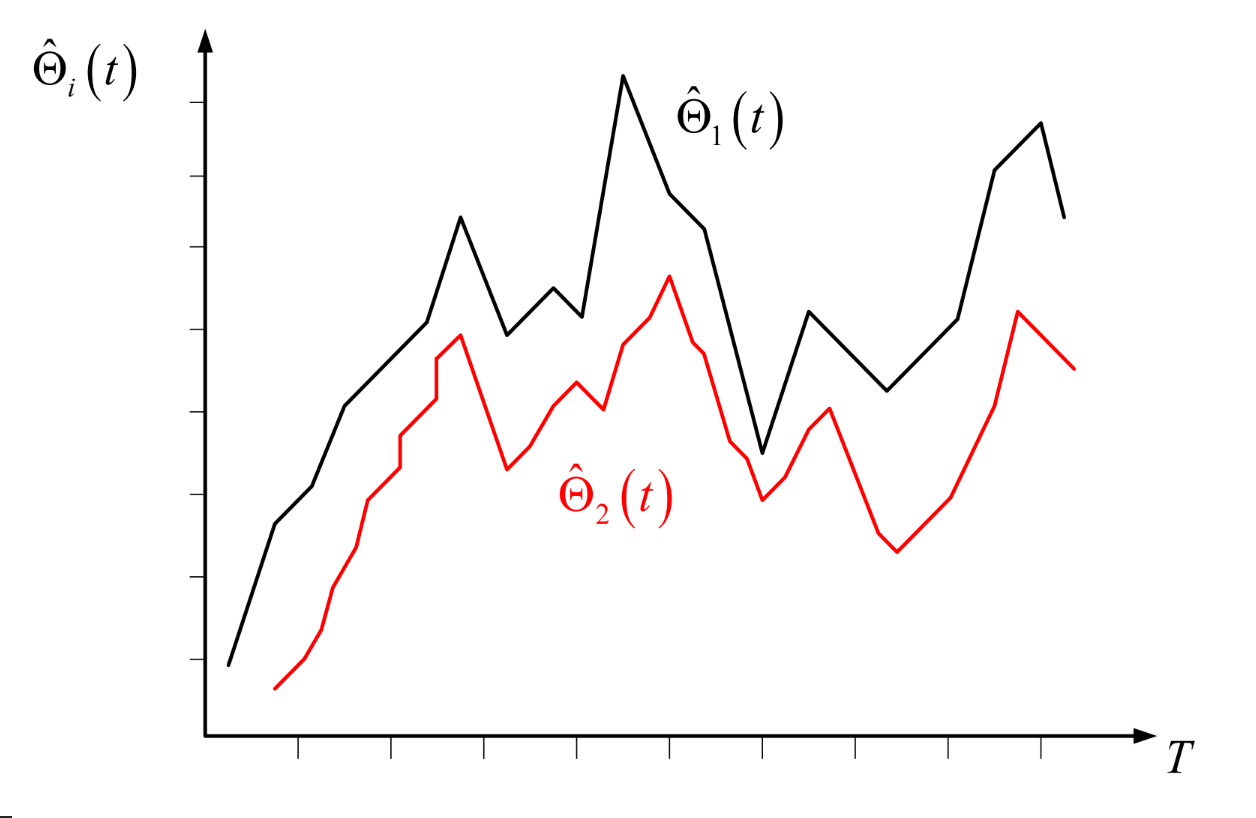
\includegraphics[width=90mm]{chapters/chapter4/figures/leyesObservatorio.png}
     \end{center}
     \textbf{\caption{Dos leyes hipotéticas encontradas por el Observatorio con base en la simulación.}}
\end{figure}

Una vez identificadas el investigador puede usarla para, por ejemplo, mejorar algún índice (en el caso de sistemas con participación humana) de calidad de vida o, por qué no, concluir que una mejora en tal índice es imposible.\\

\begin{equation}
\begin{matrix} $\Theta \in \mathbb{R}^p$ \\ \ $\Theta=(\Theta_1,\Theta_2,...,\Theta_p)$ \end{matrix}
\label{comportamientosEq}
\end{equation}

Las leyes dadas en la expresión ( \ref{comportamientosEq} ) junto con los parámetros dados en la expresión ( ~\ref{funParametros} ) van a permitir definir estrategias y políticas sobre el sistema puesto que a través de la variación de los parámetros se podrá deducir el impacto que ese cambio o variación ejerce sobre el comportamiento base del análisis de sensibilidad; puesto que como se observa de la expresión ( ~\ref{LeyesyParam}) las leyes también dependen de los parámetros. Por eso es posible (y deseable e incluso necesario) realizar estudios de análisis de sensibilidad.\\

\begin{equation}
\textit{\begin{matrix} $\Theta_i:$ & \mathbb{R}^{m+n+q+1} &$\to$& \mathbb{R} \\ \ & $t,x,\xi,F_X$ & \to & $\Theta_i = \Theta_i(t,x,\xi,F_X)$ \end{matrix}}
\label{LeyesyParam}
\end{equation}

En este punto es donde se evidencia el rol tan importante del observatorio en el modelo SAO. Ese módulo del software (que en ocasiones incluye también hardware) tiene que emplear el esquema de la simulación para estimar o aproximar una o todas las leyes supuestas en la expresión (\ref{comportamientosEq}). Es decir, construir las tablas que aproximan la dinámica subyacente en la ley (por ejemplo un indicador del sistema MIA). Gráficamente, la Figura \arabic{chapter}—6, muestra lo que arrojaría el Observatorio con base en los mecanismos de simulación que tiene el prototipo.\\

\begin{figure}[H]
     \begin{center}
         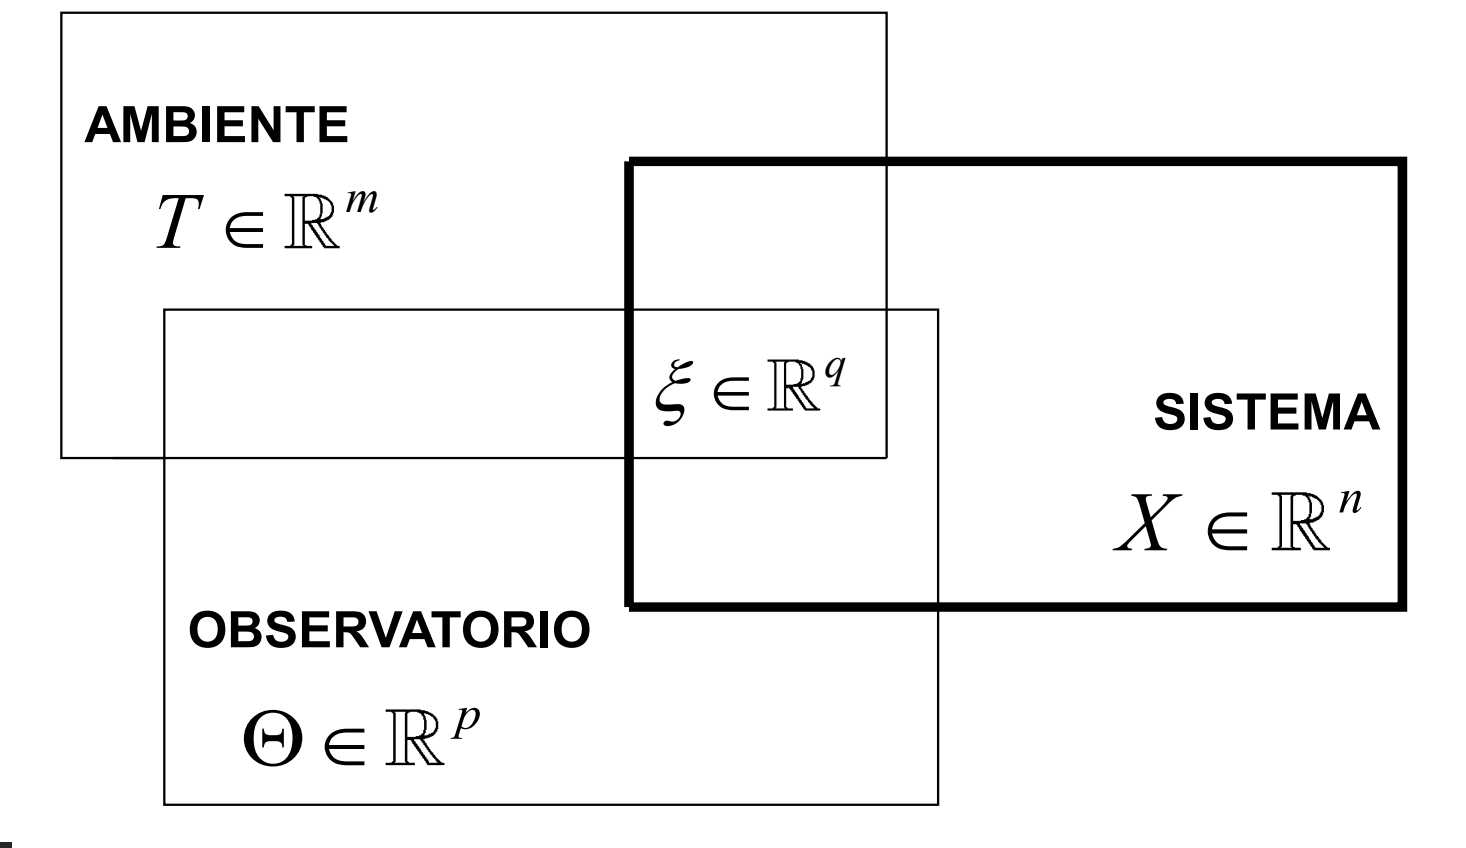
\includegraphics[width=90mm]{chapters/chapter4/figures/modeloMatSAO.png}
     \end{center}
     \textbf{\caption{Representación gráfica y matemática del modelo SAO.}}
\end{figure}

Un análisis intuitivo de la Figura \arabic{chapter}—6 indica que el vector de leyes ( \ref{comportamientosEq}) es un proceso estocástico multivariado cuya estructura probabilística, escrita formalmente en la expresión (\ref{ProbvectorLeyes}), no se conoce pero que se puede inferir (al menos su características y propiedades básicas) a partir de los datos arrojados por el simulador. Ese análisis realizado, por ejemplo, mediante series de tiempo multivariadas. Con seguridad, para los resultados supuestos de la Figura \arabic{chapter}—6, demostrarán lo que es evidente en la mencionada figura: que las leyes $\Theta_1$ y $\Theta_2$ tienen un alto grado de correlación o similitud.\\

\begin{equation}
\textit{$f_\Theta(\omega)=f_{\Theta_1,\Theta_2,...,\Theta_p}(\omega_1,\omega_2,...,\omega_p)$}
\label{ProbvectorLeyes}
\end{equation}

El modelo SAO, en resumen, se puede describir en breve como en la Figura \arabic{chapter}—7.\\

\textbf{Definición \arabic{chapter}-\arabic{definitionN}: Modelo matemático $\textfrak{MM}_{SAO}$ de la configuración SAO }\\
\stepcounter{definitionN}

El modelo matemático para una configuración SAO, $\textfrak{MM}_{SAO}$ es un objeto matemático definido mediante la tupla $\textfrak{MM}_{SAO}=(M_S,M_\Delta,M_O,I)$ en la cual:\\

\begin{enumerate}
    \item \textit{$M_{\mathbb{S}}$} es una maquina de estados finitos que modela el sistema $\mathbb{S}$.
    \item \textit{$M_\Delta$} es una máquina de estados finitos que modela el ambiente $\Delta$.
    \item \textit{$M_O$} es una máquina de estados finitos que modela el observatorio O.
    \item \textit{$I= \left\lbrace \ell_{i,j} \right\rbrace_{i,j \in \left\lbrace S, \Delta, O \right\rbrace}$} con $\ell_{i,j} = \left\lbrace \ell_{i,j}^k \right\rbrace_{k=1}^{l_{i,j}}$ es el conjunto de $l_{i,j}$ interfaces de comunicación entre el módulo $i$ y el módulo $j$ $(i \neq j)$. En sí misma, cada interfaz $\ell_{i,j}^k$ es (en general, mas no necesariamente en particular) una máquina de estados finitos.
\end{enumerate}


\section{SIMULACIÓN DE EVENTOS DISCRETOS}\label{sec:SimulEventDiscret}

Históricamente los investigadores en Simulación se han enfocado en los distintos componentes del comportamiento (optimización, aprendizaje, razonamiento, visión,....), de forma aislada. Eso ha causado que, en ciertas circunstancias (especialmente cuando se simulan sistemas complejos) los resultados no hayan sido del todo satisfactorios. En la actualidad, se sugiere \cite{trivino2012esthocasticModels} que \textbf{\textit{la Simulación, es producto de la interacción entre una comunidad de agentes (SS) y su entorno.}} Entonces, comportamientos complejos, que no han sido modelados, emergen de la interacción de varios comportamientos simples como los agentes artificiales; sin embargo, el marco clásico de la simulación de sistemas complejos sigue aún muy vigente.\\

Por consiguiente, en este capítulo se exponen los principales elementos de una simulación tradicional y se deja para otro capítulo el desarrollo con más detalle del paradigma de agentes. Así, simulación clásica y simulación basada en agentes no son conceptos disyuntos ni incompatibles, al contrario, el paradigma de agentes hace más robustos los modelos de simulación.\\

\textbf{Definición \arabic{chapter}-\arabic{definitionN}: Evento }\\
\stepcounter{definitionN}

Un evento es un acontecimiento que ocurre en algún instante en el Tiempo-Espacio (de la simulación) y que cambia el estado del sistema. La Figura \arabic{chapter}—8 representa esa visión.\\

Cada vez que ocurre un evento se disparan un conjunto de acciones que tienden a actualizar el valor de las variables de estado. En simulación clásica, la ocurrencia de un evento dispara automáticamente un procedimiento asociado específicamente con el tipo de evento que está ocurriendo. Por su lado, bajo el paradigma de agentes (discutido en un capítulo aparte de este pero estrechamente relacionado) el evento activará a la comunidad de agentes asociados con ese evento. Los agentes percibirán su entorno y, al unísono, ejecutarán sus acciones que afectarán el estado del ambiente y el de ellos mismos por supuesto (véase el Ejemplo \arabic{chapter}—5 como ilustración).\\

\begin{figure}[H]
     \begin{center}
         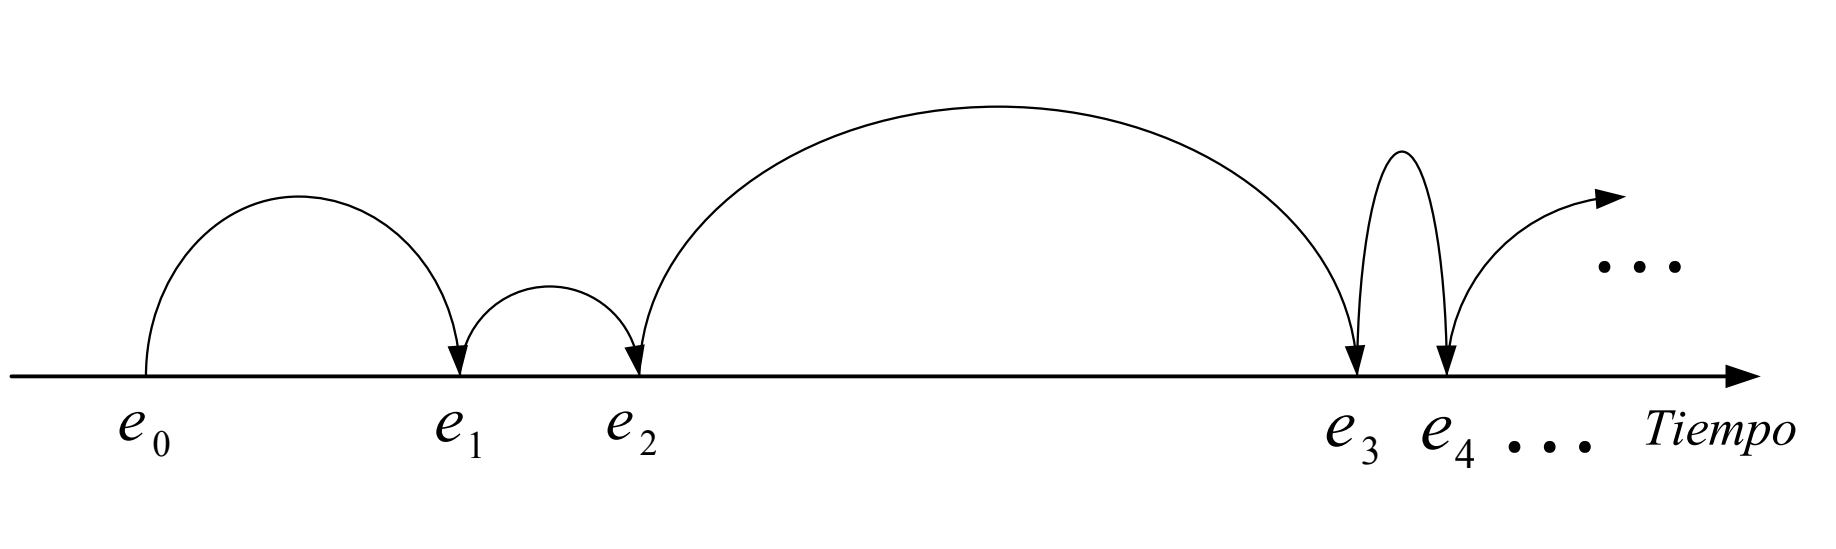
\includegraphics[width=90mm]{chapters/chapter4/figures/relacTiempoEvento.png}
     \end{center}
     \textbf{\caption{Relación entre tiempo y eventos.}}
\end{figure}


\subsection{Arquitectura de la Aplicación }\label{subsec:ArquitDeLaApp}

Un esquema general para abordar cualquier problema de simulación se puede esquematizar implementando el siguiente conjunto de algoritmos que parten de la idea de eventos discretos. El primer algoritmo importante es inicialización, cuya estructura se muestra en el Algoritmo \arabic{chapter}—1. Su propósito es colocar los niveles iniciales de todo el conjunto de variables que participan en la simulación.\\

\begin{center}
\textit{
\raggedright
PROCEDIMIENTO INICIALIZACIÓN($\langle$ Argumentos$\rangle$)\\
\quad INICIO\\
\quad \quad $T \gets$ $\langle$ValoresInicialesTiempoEspacio$\rangle$;\\
\quad \quad $X \gets$ $\langle$ValoresInicialesEstudioSistema$\rangle$;\\
\quad \quad $\theta \gets$ $\langle$ValoresInicialesCaracteristicasSistema$\rangle$;\\
\quad \quad $\xi \gets$ $\langle$ValoresInicialesParametrosSistema$\rangle$;\\
\quad \quad $L \gets$ $\langle$ValoresInicialesListaEventos$\rangle$; // Se emplea función percentil\\
\quad FIN\_PROCEDIMIENTO\_INICIALIZACIÓN\\}

\textbf{Algoritmo \arabic{chapter}-\arabic{algorithmN}: Procedimiento de inicialización.}\\
\end{center}\\
\stepcounter{algorithmN}

Otra función importante dentro del esquema general del simulador lo constituye el manejo del tiempo espacio. En un sentido general es un procedimiento cuya finalidad es manejar el reloj de la simulación. Su estructura lógica se muestra en el Algoritmo \arabic{chapter}—2.\\

\begin{center}
\textit{
\raggedright
$\mathbb{N}$ FUNCION ManejoTiempoEspacio($\langle$Argumentos$\rangle$)\\
\quad INICIO\\
\quad \quad $k^* \gets \{ k | L[k] == min_\gamma\{ L[\gamma]\}\}$; // Próximo evento\\
\quad \quad $T \gets L[k^*]$; // Actualizar el Tiempo Espacio: ''Reloj''\\
\quad \quad RETORNAR($k^*$);\\
\quad FIN\_FUNCION\_ManejoTiempoEspacio\\ }

\textbf{Algoritmo \arabic{chapter}-\arabic{algorithmN}: Función para manejar el tiempo y el espacio del simulador.}\\
\end{center}\\

\stepcounter{algorithmN}

De forma similar, por cada tipo de evento que presente el sistema a simular, debe incluirse una función que se encargue de actualizar adecuadamente el conjunto de variables de estado y de características del sistema. Esa labor la desarrolla el Algoritmo \arabic{chapter}—3.\\

\begin{center}
\textit{
\raggedright
$\mathbb{R}$ FUNCIÓN EVENTO\_$i$($\langle$Argumentos$\rangle$)\\
\quad INICIO\\
\quad \quad $X \gets$ $\langle$ActualizarEstudioSistema$\rangle$;\\
\quad \quad $\theta \gets$ $\langle$ActualizarCalculoCaracteristicas$\rangle$;\\
\quad \quad $L \gets$ $\langle$ActualizarListaEventos$\rangle$; // Usar Funciones Percentiles\\
\quad FIN\_FUNCIÓN\_EVENTO\_$i$\\ 
}
\textbf{Algoritmo \arabic{chapter}-\arabic{algorithmN}: Estructura general del evento i.}\\
\end{center}\\

\stepcounter{algorithmN}

La aplicación práctica del teorema fundamental de la simulación, presentado en la sección anterior se lleva a cabo en el Algoritmo \arabic{chapter}—4.\\

El Algoritmo \arabic{chapter}—6 tiene la misión de dirigir el llamado de todas las funciones y procedimientos descritas anteriormente. Esa ejecución debe hacerse de manera ordenada y sistemática y a su debido momento. Esa es la labor de este procedimiento principal, que se describe en el Algoritmo \arabic{chapter}—6.

\begin{center}
\textit{
\raggedright
$\mathbb{R}$ FUNCIÓN PercentilContinuaGeneral($\langle$ParámetrosPoblacionales$\rangle$)\\
\quad INICIO\\
\quad \quad $u \gets$ Aleatorio($\bullet$);\\
\quad \quad $x \gets$ $F_x^{-1}(u)$;\\
\quad \quad RETORNAR($x$);\\
\quad FIN\_FUNCIÓN\_PercentilContinuaGeneral\\ 
}
\textbf{Algoritmo \arabic{chapter}-\arabic{algorithmN}: Implementación de una función percentil.}\\
\end{center}\\

\stepcounter{algorithmN}

Finalmente se debe ejecutar un procedimiento que muestre los reportes de las estadísticas finales que muestre los resultados de la simulación. Esta tarea la realiza el Algoritmo \arabic{chapter}—5.\\

\begin{center}
\textit{
\raggedright
 PROCEDIMIENTO GeneradorReporte($\langle$Argumentos$\rangle$)\\
\quad INICIO\\
\quad \quad $\theta \gets$ $\langle$CalculoFinalDeCaracterísticas$\rangle$;\\
\quad \quad ESCRIBIR($\theta$);\\
\quad FIN\_PROCEDIMIENTO\_GeneradorReporte\\ 
}
\textbf{Algoritmo \arabic{chapter}-\arabic{algorithmN}: Procedimiento de reporte de la simulacíon.}\\
\end{center}\\

\stepcounter{algorithmN}


\subsection{Metodología de la Simulación}\label{subsec:MetodDeLaSimul}

La metodología de la simulación, como es de esperarse, está fuertemente inspirada en el método científico. Sus pasos o etapas están estrechamente relacionados con ese método. La Figura \arabic{chapter}—9 presenta, en forma de diagrama de flujo las diez etapas que la componen y que fueron adoptadas en la construcción del sistema MIA. Un mayor detalle en la descripción de cada uno de los pasos presentados se puede encontrar en \cite{law1991simulationModeling} y en \cite{trivino2010complexSystems}. Es necesario seguir con extremo rigor estos pasos y sus recomendaciones.\\

En síntesis, y en explicación de la Figura \arabic{chapter}—9, los pasos de la metodología consisten en:\\

\textbf{\textit{\underline{Etapa \# 01:} Formulación del problema y el plan de estudio.}}\\

El problema de interés se fija y se formaliza. Esta labor debe ser realizada por el director del área. Usualmente se llevan a cabo una o más reuniones con esta finalidad en la cual deben asistir el director del proyecto, el analista de simulación, y expertos en la materia: En esas reuniones se deberían discutir los siguientes temas:\\

\begin{enumerate}
    \item Los objetivos generales del estudio.
    \item Preguntas específicas que serán resueltas por el estudio.
    \item Las medidas de desempeño que se utilizarán para evaluar la eficacia de diferentes
configuraciones del sistema.
    \item Alcance del modelo.
    \item Configuraciones y escenarios del sistema a ser modelados.
    \item Herramientas de cómputo, específicamente Hardware y Software que se va utilizar.
    \item Periodo de tiempo para el estudio y los recursos necesarios.
\end{enumerate}

\begin{center}
\textit{
\raggedright
$\mathbb{N}$ FUNCIÓN SimuladorPrincipal($\langle$Argumentos$\rangle$)\\
\quad INICIO\\
\quad \quad CodError$ \gets$ $0$;\\
\quad \quad Inicialización($\langle$Argumentos$\rangle$);\\
\quad \quad MIENTRAS($\langle$NoHayaCondiciónTerminación$\rangle$,$\land$,CodError==$0$) HACER\\
\quad \quad \quad INICIO\\
\quad \quad \quad \quad i $\gets$ ManejoTiempoEspacio($\langle$Argumentos$\rangle$);\\
\quad \quad \quad \quad SELECCIONAR(i) DE\\
\quad \quad \quad \quad \quad INICIO\\
\quad \quad \quad \quad \quad \quad CASO 1: Evento\_1($\langle$Argumentos$\rangle$);\\
\quad \quad \quad \quad \quad \quad CASO 2: Evento\_2($\langle$Argumentos$\rangle$);\\
\quad \quad \quad \quad \quad \quad \quad \quad \quad $\vdots$ \\
\quad \quad \quad \quad \quad \quad CASO i: Evento\_i($\langle$Argumentos$\rangle$);\\
\quad \quad \quad \quad \quad \quad \quad \quad \quad $\vdots$ \\
\quad \quad \quad \quad \quad \quad CASO m: Evento\_m($\langle$Argumentos$\rangle$);\\
\quad \quad \quad \quad \quad FIN\_SELECCIONAR\\
\quad \quad \quad FIN\_MIENTRAS\\
\quad \quad  GeneradorReporte($\langle$Argumentos$\rangle$);\\
\quad FIN\_SimuladorPrincipal\\ 
}
\textbf{Algoritmo \arabic{chapter}-\arabic{algorithmN}: Estructura general de un simulador para sistemas dinámicos.}\\
\end{center}

\stepcounter{algorithmN}


\begin{figure}[H]
     \begin{center}
         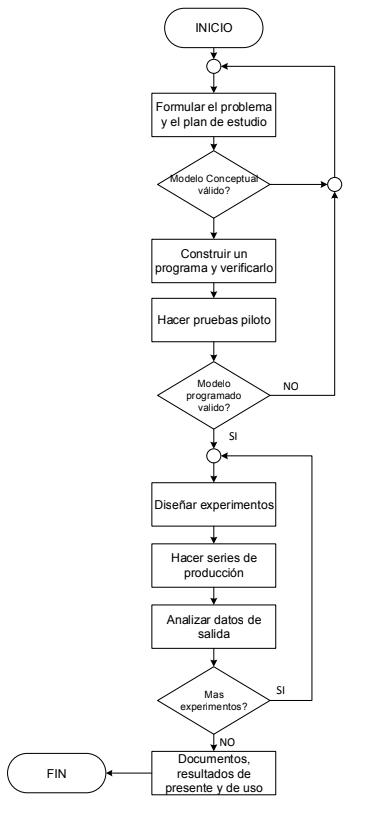
\includegraphics[width=6cm]{chapters/chapter4/figures/metodDeSimulacion.png}
     \end{center}
     \textbf{\caption{Metodología de la Simulación (Adaptada de \cite{law1991simulationModeling})}}
\end{figure}

\textbf{\textit{\underline{Etapa \# 02:} Recolección de datos y definición del modelo.}}\\

Recopilar información sobre el diseño del sistema y los procedimientos de operación. Verificar la calidad de la información puesto que, en ciertas ocasiones cuando se trabaja con información que tienen algunas personas esa información puede ser inexacta.\\

Luego, recolectar datos (si ello es posible) para estimación de parámetros específicos del modelo y las distribuciones de probabilidad de entrada. Delinear esta información anterior y los datos en un ''documento de supuestos''. Cuál es el modelo conceptual. Así mismo, de ser posible, recolectar datos sobre el rendimiento del sistema existente (Para fines de validación en el Paso 6). El nivel de detalle del modelo debe depender de lo siguiente:\\

\begin{enumerate}
    \item Objetivos del proyecto
    \item Medidas de desempeño
    \item Problemas de Credibilidad
    \item Restricciones de ordenador
    \item Las opiniones de los PYME
    \item Las limitaciones de tiempo y dinero
\end{enumerate}

Al ser un modelo, no tiene que haber una correspondencia uno a uno entre cada elemento del modelo y el elemento correspondiente del sistema. Por ello es necesario identificar los más relevantes.\\

\textbf{\textit{\underline{Etapa \# 03:} ¿Es válido el modelo conceptual?}}\\

Realizar un recorrido del modelo conceptual utilizando el documento de supuestos antes de una audiencia con los gerentes y los analistas.\\

\textbf{\textit{\underline{Etapa \# 04:} Construir un prototipo de software y verificarlo.}}\\

Programar el modelo en un lenguaje de programación (por ejemplo, C, JAVA, PHYTON), o en el software de simulación (por ejemplo, un FrameWork de agentes). Emplear un lenguaje de alto nivel tiene un beneficio claro puesto que se conoce, tiene un costo de compra bajo, y puede resultar en un tiempo de ejecución del modelo más pequeño. El uso de software de simulación reduce el tiempo de programación y los resultados en un costo del proyecto menor pero se restringe a las limitaciones y posibilidades de la herramienta.\\

\textbf{\textit{\underline{Etapa \# 05:} Hacer pruebas piloto.}}\\

Esta etapa permite la validación necesaria en el Paso 6 de esta metodología.\\

\textbf{\textit{\underline{Etapa \# 06:} ¿El modelo programado es válido?}}\\

Si hay un sistema real, a continuación, comparar el modelo (implementado) y el sistema. Realizar pruebas de sensibilidad.\\

\textbf{\textit{\underline{Etapa \# 07:} Diseño de experimentos.}}\\

Para cada uno de los escenarios de interés determinar el número de corridas, el periodo de calentamiento necesario.\\

\textbf{\textit{\underline{Etapa \# 08:} Ejecutar las corridas definitivas.}}\\

Estas corridas son necesarias para la realización del paso 9 de ésta metodología el cual tiene como propósito obtener los resultados definitivos.\\

\textbf{\textit{\underline{Etapa \# 09:} Análisis de la información de salida.}}\\

Usualmente se acompaña de la aplicación de métodos estadísticos que le dan formalidad al análisis. El propósito de esta etapa es obtener el conjunto de datos resumidos en tablas que describen las dinámicas de las leyes que se desea estimar. Cada dato debe haber sido calculado con un error máximo permitido y una significancia determinada por el investigador. También en esta fase se pueden comparar los diferentes escenarios simulados.\\

\textbf{\textit{\underline{Etapa \# 10:} Informe y resultados.}}\\

Elaboración del documento final en el cual se plasman los resultados más importantes que muestran
los estudios de simulación realizados. Frecuentemente, estos datos son enviados a un experto quien
deberá tomar decisiones que afecten al sistema basado en lo que el informe le está comunicando.\\

\section{RESUMEN Y PANORAMA HISTÓRICO }\label{sec:ResumenyPanHisoric}
\section{EJERCICIOS}\label{sec:EjerciciosModySimul}

\begin{enumerate}
    \item Analizar, diseñar e implementar (en algún lenguaje de programación, se sugiere Python o Java), una aplicación que permita simular, es decir que cuente con las funcionalidades descritas en la sección \ref{subsec:ArquitDeLaApp}, para cualquier sistema $\mathbb{S}$ que pueda abstraerse a través del modelo matemático SAO propuesto en la Definición \arabic{chapter}—11.\\
    
    \item Para el Ejemplo \arabic{chapter}—5, aplique la Definición 1—5 para proponer un ambiente para este sistema y la Definición \arabic{chapter}—10 para obtener su modelo matemático.\\
    
    \item Emplear el Ejemplo \arabic{chapter}—5, el Ejemplo \arabic{chapter}—8 y los resultados de los Ejercicios 2 y 3 como primer escenario de prueba para la aplicación construida en el Ejercicio 1.\\
    
    \item Proponer otros dos sistemas $\mathbb{S}_1$ y $\mathbb{S}_2$ , obtener sus respectivos modelos matemáticos $\textfrak{MM }_{SAO}^1$ y $\textfrak{MM }_{SAO}^2$, y simularlos en la aplicación construida en el Ejercicio 1.\\
    
    \item Para el sistema dado en el Ejemplo \arabic{chapter}—4
    \begin{enumerate}
        \item Aplicar la Definición \arabic{chapter}—8 para encontrar su modelo matemático.
        \item Aplicar la Definición \arabic{chapter}—11 para determinar su modelo matemático SAO.
    \end{enumerate}
\end{enumerate}

%\chapter{TEOREMA FUNDAMENTAL DE LA SIMULACIÓN}
%\chapter{ARQUITECTURA GENERAL DE UN SIMULADOR DE SISTEMAS COMPLEJOS}
%\chapter{FUNCIONES PERCENTILES,TRUNCADAS Y CONTAMINADAS CONJUNTAS}
%\chapter{MODELOS DE MOVILIDAD}
%\chapter{LENGUAJES DE PROGRAMACIÓN PARA SIMULACIÓN DE REDES}
%\chapter{DISTRIBUCIÓN LAMBDA GENERALIZADA}


\part{TEORÍA DE LA DECISIÓN EN COMUNIDADES DE AGENTES ARTIFICIALES}

%\chapter{TEORIA DE LA UTILIDAD}
%\chapter{MODELOS BAJO INCERTIDUMBRE}
%\chapter{TEORÍA DEL RIESGO Y ÁRBOLES DE DECISIÓN}
%\chapter{ANÁLISIS BAYESIANO}
%\section{}
%\subsection{}
%\chapter{TEORÍA DE JUEGOS}
%\chapter{REDES DE AUTÓMATAS ESTOCÁSTICOS}
%\chapter{DECISIONES MULTIOBJETIVO EN COMUNIDADES DE AGENTES ARTIFICIALES: COOPERACIÓN Y NEGOCIACIÓN}

\chapter{DECISIONES EN COMUNIDADES DE AGENTES ARTIFICIALES}

\section{INTRODUCCIÓN}

\section{PLANTEAMIENTO DEL PROBLEMA}\label{Sec:Planteamiento}

\section{CLASIFICACIÓN DE LOS JUEGOS DE ESTRATEGIA}\label{Sec:Clas_JE}


\section{JUEGOS DE SUMA CONSTANTE ENTRE DOS AGENTES}\label{Sec:Juegos_SC2A}
\subsection{Estrategias dominadas}
\subsection{Solución de un juego de suma constante entre dos agentes}
\subsection{Solución mixta de un juego bipersonal de suma constante}
\subsection{Modelo de programación lineal para juegos de suma constante}

\section{JUEGOS DE SUMA NO CONSTANTE ENTRE DOS AGENTES}\label{Sec:Juegos_SNC2A}
\subsection{Equilibrio puro de Nash de un juego de suma no constante entre dos agentes}
\subsection{Equilibrio de Nash con estrategias mixtas en un juego de suma no constante entre dos agentes}

\section{CASOS DE ESTUDIO}\label{Sec:CE_DCA}
\subsection{Caso 1: Competencia entre dos comunidades}
\subsection{Caso 2: Comunidades de agentes y programación lineal}


\part{TEORÍA DE ESTADÍSTICAS Y CONVERGENCIA}
% Juan Camilo Cárdenas Gómez
\chapter{SIMULACIÓN ESTADÍSTICA Y COVERGENCIA}

\floatname{algorithm}{Algoritmo}
\renewcommand{\theequation}{\arabic{chapter}|\arabic{equation}}
\renewcommand{\thealgorithm}{\arabic{chapter}|\arabic{algorithm}}
\renewcommand{\theexample}{\arabic{chapter}|\arabic{example}}

\algrenewcommand\algorithmicreturn{\textit{RETORNAR}}
\algrenewcommand\algorithmicloop{\textit{INICIO}}
\algrenewcommand\algorithmicwhile{\textit{MIENTRAS}}
\algrenewcommand\algorithmicdo{\textit{HACER}}

En este capítulo se presentan dos temas fundamentales en el desarrollo del sistema MIA. El primero hace alusión a la arquitectura algorítmica básica necesaria para obtener datos de \emph{buena calidad}  (estadística) puesto que la inferencia y decisiones se soportan en ellos. El segundo tema, no menos importante que el primero, tiene que ver con la determinación del número de simulaciones necesario para asegurar esa calidad requerida.

Para garantizar el primero en el sistema MIA se estableció (y adaptó) el procedimiento general de simulación estadística propuesto en (Ortiz Triviño, 2010) mientras que para el segundo se aplicaron la ley de los grandes números y el teorema del límite central descritos en (Mood, Graybill \& Boes, 1974).

\section{ARQUITECTURA DE UN SIMULADOR SIMPLE}

El cálculo de la estimación de un valor de un estimador para un indicador se obtiene a partir de una (sub) muestra aleatoria de las variables de estado del sistema. Esto es, si $\{ X_i \}_{i=1}^{i=n}$ es el conjunto de variables de estado del sistema y $\beta_k$ con $k=1,2,\cdots,m$ es el \emph{k-ésimo} indicador, se cumple la expresión \ref{exp_1}.  Por esa razón se hace indispensable la implementación de un procedimiento adecuado para obtener las muestras respectivas (Ortiz Triviño, 2010).

\begin{equation} \label{exp_1}
\begin{split}
\hat{\beta}_k: \quad&\ \ \ \ \ \mathbb{R}^n\quad\ \rightarrow\ \ \qquad\ \ \ \ \mathbb{R} \\
\quad&\{ X_i \}_{i=1}^{i=n}\ \ \rightarrow\ \ \hat{\beta}_k = \hat{\beta}_k (\{ x_i \}_{i=1}^{i=n})
\end{split}
\end{equation}

\subsection{Una simulación}

De acuerdo con (Ortiz Triviño, 2010), el nivel más bajo en el proceso de simulación consiste en obtener un valor aproximado de la variable (de estado) aleatoria involucrada, es decir, implementar un algoritmo que permita obtener un valor (estimado) de la estadística utilizada para aproximar la respuesta pedida. La fisonomía del algoritmo puede ser como la del Algoritmo \ref{algo_1}.

\algrenewcommand\algorithmicfunction{$\langle Tipo\_Dato\rangle\ \textit{FUNCION}$}

\begin{algorithm}
\begin{algorithmic}[0]
\Function{$\langle Simulaci\acute{o}n\_i-\acute{e}sima\rangle$}{$\langle lista\_de\_par\acute{a}metros\rangle$}
    \Loop
        \State $\langle Instrucci\acute{o}n\ 1\rangle;$
        \State $\langle Instrucci\acute{o}n\ 2\rangle;$
        \State \qquad \vdots
        \State $\langle Instrucci\acute{o}n\ n\rangle;$
        \State $x \gets g(\text{\textbullet});$
        \State \Return $(X);$
    \EndLoop \State $FIN\_ALGORITMO\ \_\langle Simulaci\acute{o}n\_i-\acute{e}sima\ \rangle$
\EndFunction
\end{algorithmic}
\caption{\!\textbf{: Simulación de un dato (Adaptado de }(Ortiz Triviño, 2010)\textbf{)}}\label{algo_1}
\end{algorithm}

La estructura interna del algoritmo dependerá totalmente del indicador a simular, sin embargo, es usual que en este nivel se retorne el valor de una variable aleatoria $X$.

\subsection{Muestra aleatoria artificial}

Luego de haber diseñado el simulador básico debe utilizarse repetidamente para generar un vector de valores de la variable aleatoria en estudio, el fin, como seguramente puede suponer, es encontrar un conjunto de $n$ valores\footnote{Se suele considerar un buen número a $n\geq30.$} (suficientemente  grande\footnote{El teorema del límite central se desarrolla en detalle en el capítulo de Teoría Asintótica.}) de la variable $X$. El Algoritmo \ref{algo_2}  representa este caso.

\subsection{Procedimiento general de simulación estadística}

Tradicionalmente, se ha empleado simulación, principalmente, en campos de la investigación de operaciones.  Allí existen problemas en los cuales encontrar su solución es demasiado complejo y/o es muy costosa. Es justamente en esos casos cuando el ingeniero acude a herramientas como ésta para \textit{aproximar} la solución al problema.

Por lo anterior es conveniente hacer una distinción en la forma de solucionar un problema.  En lo que a este texto respecta, se distinguen dos formas esenciales: Métodos \textit{analíticos}, de un lado, y \textit{Métodos de Simulación}, del otro.  En el primer caso, la respuesta se encuentra luego de una aplicación sistemática del cálculo, la estadística, la teoría de probabilidades, el álgebra, etc.  Por el otro lado, en cambio,  se imita normalmente a través de números aleatorios, el comportamiento del sistema (implícito en el enunciado del problema) se miden sus variables de interés en cada experimento, se construyen estadísticas apropiadas que ayuden a aproximar la respuesta que se está buscando y, finalmente,  se busca aplicar  teoremas límites que  validen aún más los resultados.

\algrenewcommand\algorithmicfunction{$\uparrow Vector\ \textit{FUNCION}$}

\begin{algorithm} 
\begin{algorithmic}[0] 
\Function{$\langle Simulaci\acute{o}n \_Vector\rangle$}{$n \in \mathbb{N}$}
    \Loop
        \State $i \gets 1;$
        \While{$(i < n)$} 
            \Loop
                \State $X[i] \gets \textit{Simulación\_i-ésima}(\langle \textit{lista\_de\_parámetros}\rangle);$
                \State $i \gets i + 1;$
            \EndLoop \State $\textit{FIN \_MIENTRAS}$
        \EndWhile
        \State \Return $(\uparrow X);$
    \EndLoop \State $\textit{FIN\_ALGORITMO} \_\langle\textit{Simulación\ \_Vector}\rangle$
\EndFunction
\end{algorithmic}
\caption{\!\!\textbf{: Simulación de  una muestra aleatoria artificial (Adaptado de} (Ortiz Triviño, 2010)\textbf{)}}\label{algo_2}
\end{algorithm}

Formalmente hablando, Sea $X$ una variable aleatoria con función de distribución $F(X)$ y sea $\theta(F)$ una característica de la población $F(X)$. Para evaluar la característica  $\theta(F)$ existen, cuando menos, dos caminos: (1) Calcular exactamente  $\theta(F)$, es decir, encontrar la solución analítica;  y  (2) Estimar, normalmente mediante simulación, el valor de  $\theta(F)$, en este caso se debe construir una estadística  $\hat{\theta}(F)$ apropiada.

Cuando se usa el segundo camino, se aplican los siguientes pasos (Ortiz Triviño, 2010):

\begin{enumerate}
    \item Encontar la función percentil $X = F_x^{-1}(U)$
    \item Obtener una muestra aleatoria de tamaño $n, X_1, X_2, \cdots, X_n$, de la población $F_x(x)$
    \item Calcular $\theta(F_x)\approx\hat{\theta}(\{X_i\}_{i=1}^{i=n})$
\end{enumerate}

Al final de este procedimiento se tiene una aproximación a la respuesta deseada, sin embargo, debe notarse que $\hat{\theta}(F)$ es en sí misma una variable aleatoria y, en consecuencia, debe tener una función de distribución $F_{\hat{\theta}}(\omega)$ asociada (lamentablemente cuyo comportamiento específico se desconoce en la mayoría de los casos). Sin embargo $\theta(F_x)$ es una constante pero desconocida.

La metodología descrita se denomina \textit{Procedimiento general de simulación estadística} y se denota por $\textit{PGSE}(\theta,F_x,m,n)$.

El conocimiento explícito de $\theta(F_x)$ se denomina solución analítica mientras la aproximación $\hat{\theta}(F)$ se conoce como solución simulada. Un ejemplo extraído de la teoría de probabilidades ilustra el concepto de \textit{solución analítica} vs \textit{solución numérica}.

El  Ejemplo \ref{exa_1} ilustra la filosofía de la simulación y la forma de empleo de la metodología propuesta.



% \newcommand{\example}{\subsubsection}

% \example{} \label{exa_1}

\example{holo}\label{exa_1}

\example


\part{SIN TÍTULO}
\chapter{MUESTREO}
\chapter{ESTIMACIÓN PUNTUAL Y POR INTERVALOS}


\part{AGENTES MÓVILES Y MODELOS DE MOVILIDAD}
\chapter{MODELOS MATEMÁTICOS Y SIMULACIÓN}

%Contadores y formato para numeracion de elementos
\renewcommand{\thefootnote}{\arabic{footnote}}
\renewcommand{\theequation}{\arabic{chapter}-\arabic{equation}}
\renewcommand{\thefigure}{\arabic{chapter}.\arabic{figure}}
\renewcommand{\figurename}{Figura}
\renewcommand{\tablename}{\textbf{Tabla}}
\renewcommand{\thetable}{\textbf{\arabic{chapter}-\arabic{table}}}
\stepcounter{definitionN}
\stepcounter{exampleN}
\stepcounter{tableN}
\stepcounter{footN}
\stepcounter{algorithmN}
\providecommand{\abs}[1]{\lvert#1\rvert}
\providecommand{\norm}[1]{\lVert#1\rVert}



\section{INTRODUCCIÓN}\label{sec:intro}
\section{MODELOS DE MOVILIDAD SINTÉTICOS ESTÁNDAR}\label{sec:movilityModels}
\subsection{Random Walk Mobility Model}
\subsection{Random Waypoint}
\subsection{Gauss-Markov}

\section{FAMILIA PARAMÉTRICA DE GAUSS}\label{sec:gaussParamFam}
\subsection{Familia de Gauss Uniparamétrica}
\subsection{Distribución Normal Multivariada}
\subsubsection{Función de densidad}
\subsubsection{Integral de Aitken}
\subsubsection{Función Generadora De Momentos}
\subsubsection{Distribuciones Marginales}
\subsubsection{Distribuciones Condicionales}
\subsubsection{Independencia}

\section{MOVILIDAD GAUSS-MARKOV CON ATRACTORES}
\subsection{Generador de una variable de Gauss Univariada}
\subsection{Generador de un vector dimensional de Gauss}
\subsection{Método de movilidad Gauss-Markov con múltiples atractores}




\part{REDES NEURONALES COMO MODELO DE DINÁMICAS Y PREDICTORES}
\renewcommand{\theequation}{\arabic{chapter}-\arabic{equation}}

\chapter{REDES NEURONALES COMO MODELO DE DINÁMICAS Y PREDICTORES}

\section{INTRODUCCIÓN}\label{sec:intro1}

\section{ELEMENTOS DE UNA RED NEURONAL ARTIFICIAL}\label{sec:elemsred}
\subsection{Neurona artificial}
\subsection{Estado de activación}
\subsection{Función de salida}
\subsubsection{Función escalón}
\subsubsection{Función lineal mixta}
\subsubsection{Función sigmoidal}
\subsubsection{Función gaussiana}
\subsection{Conexiones entre neuronas}
\subsection{Regla de activación}
\subsection{Regla de aprendizaje}

\section{ESTRUCTURA DE UNA RED NEURONAL ARTIFICIAL}

\section{LA RED BACKPROPAGATION}

\section{APLICACIONES DE LAS REDES BACKPROPAGATION}


\part{SISTEMAS EXPERTOS Y PROYECTO MIA}
\chapter{SISTEMAS EXPERTOS Y PROYECTO MIA}

%Contadores y formato para numeracion de elementos
\renewcommand{\thefootnote}{\arabic{footnote}}
\renewcommand{\theequation}{\arabic{chapter}-\arabic{equation}}
\renewcommand{\thefigure}{\arabic{chapter}.\arabic{figure}}
\renewcommand{\figurename}{Figura}
\renewcommand{\tablename}{\textbf{Tabla}}
\renewcommand{\thetable}{\textbf{\arabic{chapter}-\arabic{table}}}
\stepcounter{definitionN}
\stepcounter{exampleN}
\stepcounter{tableN}
\stepcounter{footN}
\stepcounter{algorithmN}
\providecommand{\abs}[1]{\lvert#1\rvert}
\providecommand{\norm}[1]{\lVert#1\rVert}
%%%agregue el paquete caption
\newpage

%\title{SISTEMAS EXPERTOS Y PROYECTO MIA}\label{sec:intro}
En este capítulo se presentan los principales detalles que se deben tener en cuenta en la construcción de un sistema experto.  El tema tiene especial importancia en el marco del proyecto MIA debido a que, por ejemplo, el simulador prototipo que se ha construido, arroja gran cantidad de información y suministra algunas herramientas que permiten su análisis; sin embargo, ese análisis debe estar en manos de un conjunto de expertos, bien sean humanos o automático o bien una mezcla de ambas.  \\
La ingeniería que hay detrás de la construcción de un sistema de esta naturaleza es muy avanzada pero en esta rama de la ingeniería  aún hay mucho sin descubrir o inventar.  Por esa razón, es bueno tener una dosis de optimismo en las reales posibilidades de este tipo de sistemas pero, a la vez, tener las suficientes precauciones debido a que la herramienta por sí sola no puede obtener resultados aceptables.  El tratamiento temático de este capítulo está inspirado en (Peter \& Russell, 1989), (Rolston, Gama, \& Ziskiend, 1990) y (Ortiz Triviño, 2009).
\section{	DEFINICIÓN DE UN SISTEMA EXPERTO}
De acuerdo con (Rolston et al., 1990) un SE es un software cuya finalidad es  solucionar problemas complicados que de otra manera exigirán ampliamente la pericia humana. Para lograr esto, se simula el proceso de razonamiento humano mediante la aplicación específica de conocimientos y de inferencias. En su estructura se pueden encontrar algunos subsistemas que son comunes a todo sistema experto:
\begin{itemize}
\item 	Conocimiento específico a partir del campo de interés, por ejemplo, en medicina, conducción, petróleos, etc.
\item Módulo para realizar búsqueda,
\item 	Un componente para análisis heurístico,
\item	Un módulo que le permita tener la habilidad para inferir nuevos conocimientos a partir de conocimientos ya existentes,
\item 	Un módulo que le permita  procesar símbolos más allá de los números.
\item 	Un módulo que lo dote de la capacidad para explicar su propio razonamiento.
\end{itemize}
\section{	ANÁLISIS DE LA SOLUCIÓN PRÁCTICA DE PROBLEMAS}
Uno de los primeros pasos cuando se empieza a pensar en la necesidad de la construcción de un sistema experto está en delimitar muy bien el ámbito sobre el cual ese sistema será realmente experto y si, luego de un cuidadoso análisis de costo beneficio, se justifica la ejecución de su construcción.  Los alcances y las limitaciones de dicho sistemas son fundamentales en la toma de la decisión.\\
Experiencia y conocimiento son dos propiedades que todo sistema experto debe exhibir.  En cuanto a la segunda de ellas, el conocimiento, es ampliamente aceptado, véase (Peter \& Russell, 1989), que la utilidad de un sistema experto se debe más al conocimiento  en el área específica que al mismo desempeño genérico del experto. 
\section{ARQUITECTURA TÍPICA  DE UN SISTEMA EXPERTO}
Alguno de los componentes del conocimiento que hacen posible producir la habilidad artificial de un  experto humano en su desempeño son las siguientes: 
\begin{itemize}
    \item 	Los \textbf{Hechos}. Proposiciones que relacionan algunos elementos de la realidad con referencia al área específica. Por ejemplo, el derrame de petróleo deteriora el ambiente.  Frecuentemente, los hechos son capturados a través de sensores que llevan la información desde el contexto al interior del experto. 
    \item 	Las \textbf{Reglas de procedimiento} . Reglas bien definidas e invariables que describen secuencias fundamentales de eventos y relaciones relativas al área. Por ejemplo, siempre apague el vehículo antes de intentar suministrarle gasolina. Si el altímetro señala el nivel de vuelo, el medidor de la velocidad vertical debe marcar cero.
    \item 	Las \textbf{Reglas heurísticas}. En ellas se consigna la experiencia. Son reglas generales en forma de opiniones o reglas em\\píricas que sugieren procedimientos que se pueden seguir cuando no existen disponibles reglas de procedimiento invariables. Dichas reglas son, de acuerdo con (Rolston et al., 1990),  aproximadas y han sido generalmente producidas por un experto a través de años de experiencia. Por ejemplo, un piloto de avión, puede saber de acuerdo con su experiencia que es mejor intentar un aterrizaje de emergencia bajo condiciones controladas que volar en condiciones desconocidas.  Lo realmente interesante e importante de ello es que el uso de heurísticas contribuye grandemente a la potencia y flexibilidad de los SE y tiende a distinguirlos aún más del software tradicional.
\end{itemize}
Hay, sin embargo, otras formas específicas de conocimientos, de esta manera, un experto posee un modelo conceptual general del área específica y un esquema global para hallar una solución así como también una estructura de preferencias. Estas le permiten una “visión global”.  En conjunto, ellas conforman la infraestructura básica para la aplicación por parte del experto de conocimientos detallados.   \\
\begin{figure}[H]
\centering
\captionsetup{justification=centering,margin=2cm}
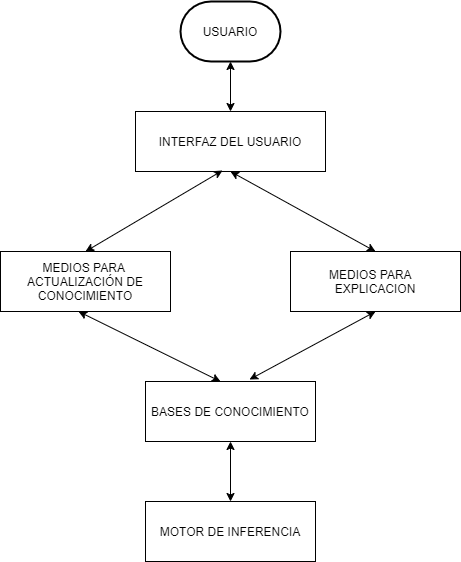
\includegraphics[scale=0.4]{chapters/chapter10/figures/1-1.png}
\caption{Arquitectura típica de sistemas expertos (Adaptado de (Rolston et al., 1990)).}
\label{fig:10-1}
\end{figure}

Los SE contemporáneos emplean una gran variedad de arquitecturas específicas en sus configuraciones, principalmente porque una arquitectura es más aplicable que otra cuando se considera una aplicación dada. Actualmente de acuerdo con (Rolston et al., 1990) las investigaciones en el tema no han llegado a una conclusión definitiva; al contrario, subsiste un considerable debate al respecto.\\
Sin embargo, en cuanto a la esencia de un SE si parece existir un consenso.  A pesar de las diferencias significativas, la mayoría de las arquitecturas tienen muchos componentes en común. La Figura \ref{fig:10-1} muestra una arquitectura general con los componentes típicos. En lo que sigue de este documento se darán algunos de talles adicionales de los módulos presentados en esa gráfica general.\\
\subsection{El usuario}

Existen varios tipos de usuario, o varios roles asociados con la interacción con un SE.  Los más comunes para (Rolston et al., 1990) son los siguientes:
\begin{itemize}
    \item \textbf{Verificador}	. El usuario intenta comprobar la validez del desempeño del sistema.
     \item 	\textbf{Tutor}. El usuario da información adicional al sistema o modifica el conocimiento que ya está presente en el sistema.
     \item 	\textbf{Alumno}. El usuario busca rápidamente desarrollar pericia personal relacionada con el área específica mediante la recuperación de conocimientos organizados y condensados en el sistema.
     \item \textbf{Cliente}	. El usuario aplica la pericia del sistema a tareas específicas reales.
\end{itemize}
El reconocimiento de las caracterizaciones, reconociendo varios tipos posibles de interacción, anteriores contrasta con la percepción de un simple papel (el cliente) de los sistemas tradicionales de software.
\subsection{	Facilidades de interfaz con el usuario}
La comunicación desde el ambiente hacia el interior del SE y desde el SE hacia el ambiente son características fundamentales.  Un SE no es un sistema aislado, todo lo contrario, debe compenetrarse con su entorno. Las facilidades de interfaz con el usuario y con el contexto deben aceptar información del usuario y traducirla a una forma aceptable para el resto del sistema o aceptar información proveniente del sistema y convertirla a una que el usuario pueda entender. No solamente se trata de una sofisticada interfaz gráfica.  Esta comunicación va mucho más allá. Actualmente, por ejemplo, en este aspecto se incluyen las redes de sensores y actuadores que le permiten al SE Artificial de acuerdo con lo que esta ocurriendo afuera de él.\\
Idealmente, esta facilidad se compone de un sistema procesador de lenguaje natural que acepta y  devuelve esencialmente información en la misma forma como es aceptada u ofrecida por una persona experta. En la actualidad existen sistemas que reproduzcan las capacidades del  lenguaje humano con destacado éxito, y también existen muchos otros que han producido impresionantes resultados mediante la utilización de subconjuntos restringidos del lenguaje.\\
Las facilidades de interfaz del usuario a menudo se diseñan para reconocer el modo en que el usuario está operando, su nivel de pericia, y la naturaleza de la transacción. La comunicación con un SE debe ser tan natural como sea posible, toda vez que el sistema trata de sustituir el desempeño humano.
\subsection{	Sistema de almacenamiento y generación de conocimiento}
El almacenamiento de conocimiento, el cual es de mayor complejidad y abstracción que los simples datos o la información, consta de una base de conocimientos y un motor de inferencia. Es el corazón de un SE. La función de este sistema consiste en almacenar confiablemente los conocimientos del experto, para recuperarlos e inferir nuevos conocimientos cuando se requiera.\\
\textbf{Base de conocimientos}. La base de conocimientos representa un depósito de las primitivas del conocimiento (por ejemplo, hechos fundamentales, reglas de procedimientos y heurísticas) disponibles para el sistema. Como se dijo anteriormente, el conocimiento guardado en la base, establece la capacidad del sistema para actuar como un experto.\\
En general, el conocimiento se almacena en forma de \textbf{hechos} y de \textbf{reglas}, pero los esquemas específicos empleados para almacenar la información varían grandemente. El diseño de este esquema de representación de conocimientos afecta el diseño del motor de inferencia, el proceso de actualización del conocimiento, el proceso de explicación y la eficiencia global del sistema.\\
Todo lo anterior conduce a pensar que la selección del esquema de representación del conocimiento es una de las decisiones más críticas en el diseño de un SE.\\
Inferencia de conocimientos. De acuerdo con (Peter \& Russell, 1989) la ingeniería de conocimientos es el proceso de adquirir el conocimiento del área específica y estructurarlo en la base de conocimientos. La Figura \ref{fig:10-2} ilustra cómo se da típicamente el proceso. Los conocimientos pueden conseguirse de una variedad de fuentes, por ejemplo redes de sensores conectados al sistema experto, incluyendo la documentación y los sistemas de información  computacional existentes, la mayor parte de él, debe obtenerse de personas experta. El conocimiento suministrado por el experto, por lo general estará en forma tal que sea orientado hacia el tema del área.
\begin{figure}[H]
\centering
\captionsetup{justification=centering,margin=2cm}
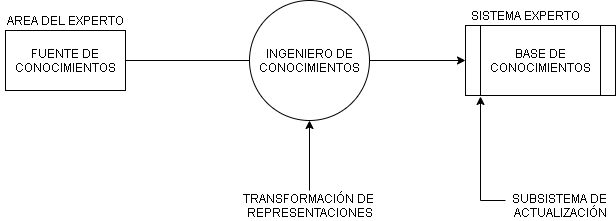
\includegraphics[scale=0.6]{chapters/chapter10/figures/1-2}
\caption{Ingeniería de conocimientos (Adaptado de (Hidalgo, 1996)).}
\label{fig:10-2}
\end{figure}
Surge de ahí un rol indispensable a tener en cuenta en el sistema MIA: El ingeniero de conocimiento (IC) quien es la persona que obtiene los conocimientos del área del experto y las transporta a la base de conocimientos. La Figura \ref{fig:10-4} bosqueja la labor del ingeniero del conocimiento. En razón de que un sistema experto requiere que los conocimientos en la base de conocimientos se guardan de acuerdo con las normas de representación de conocimientos del sistema, el IC debe transformar la representación del conocimiento como parte del proceso de transporte.\\
Para adquirir el reconocimiento necesario, el IC primero debe establecer una comprensión global del área, formar un diccionario mental de los términos y jerga esenciales del área y desarrollar una comprensión básica de los conceptos claves. Luego debe condensar los conocimientos sucintos a partir de la información suministrada por el experto.\\
La función de adquisición de conocimientos en comúnmente, el aspecto de mayor dificultad en la construcción de SE lo cual enfatiza aun más la importancia del IC.. Esto se debe principalmente al hecho de que el proceso requiere comunicaciones humanas ampliadas, entre el experto en el área y el IC y en consecuencia enfrenta los problemas asociados con esta actividad. Por tanto, según (Rolston et al., 1990)  el proceso de adquisición del conocimiento no está bien entendido ni bien definido. Si el proceso mismo de desarrollo de un SE se visualizara como un área para expertos, el conocimiento asociado con el procedimiento de adquisición sería considerado como heurístico.\\
\begin{figure}[H]
\centering
\captionsetup{justification=centering,margin=2cm}
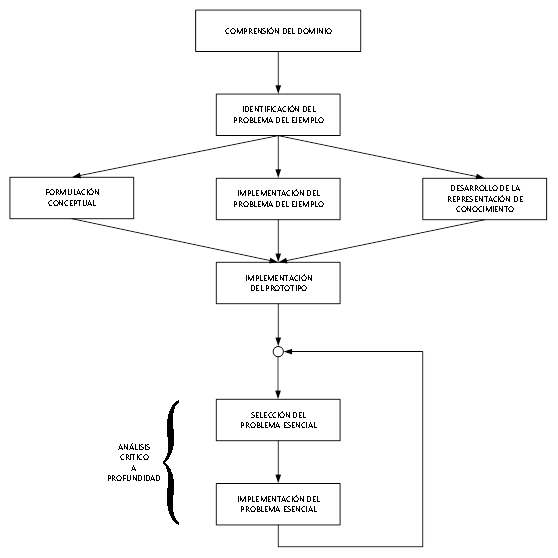
\includegraphics[scale=1]{chapters/chapter10/figures/10-3}
\caption{Identificación de problema (Tomado de (Rolston et al., 1990)).}
\label{fig:10-3}
\end{figure}
\textbf{Motor de indiferencia}. Los SE deben, por su naturaleza, tratar flexiblemente con situaciones dinámicas y estocásticas. La capacidad para adaptarse y  responder ante situaciones cambiantes depende de la habilidad para inferir nuevos conocimientos a partir de conocimientos existentes.  El ejemplo proporcionado por (Rolston et al., 1990) ilustra muy bien esta idea. Considere los dos hechos básicos siguientes:
\begin{enumerate}
\item Todos los animales respiran oxígeno.
\item Todos los perros son animales.
\end{enumerate}
Se puede inferir un nuevo hecho, “todos los perros respiran oxígeno” a partir de los dos hechos anteriores. Para responder a una situación dada, un SE debe aplicar el conocimiento apropiado. La aplicación de conocimientos apropiados implica que los conocimientos requeridos fueron o identificados como conocimientos existentes en la base de conocimientos o inferidos a partir de estos.\\
Lo discutido hasta este momento sirve de justificación para la afirmación de(Peter \& Russell, 1989) según la cual el proceso de buscar los conocimientos apropiados y a partir de estos deducir nuevos conocimientos constituye un elemento clave del procesamiento de un sistema experto.  Por lo tanto, a diferencia de postulados de la construcción de otros tipos de sistemas computacionales como los sistemas de información o las bases de datos, en un SE es deseable (y probablemente necesario) almacenar el conocimiento adquirido aunque éste pueda ser nuevamente inferido de las reglas primitivas.\\
Una de las mayores dificultades asociadas con la operación a partir de las primitivas es el hecho que, aun unos pocos elementos individuales (tales como, primitivas)  se puedan combinar dentro de un número muy grande de combinaciones únicas. El número de posibilidades a partir de un conjunto grande de elementos, rápidamente se convierte en una cifra astronómica. Este problema se conoce como explosión combinatoria. \\
El motor de inferencia es el software que ubica los conocimientos e infiere nuevos usando la base de conocimientos. El paradigma del motor de inferencia es la estrategia de búsqueda que se emplea para producir el conocimiento demandado. Varios paradigmas diferentes se emplean en un SE, pero la mayoría de ellos se basan en dos conceptos fundamentales: encadenamiento hacia atrás (o retroencadenamiento) que es un proceso de razonamiento descendente, que se inicia a partir de los objetivos deseados y trabaja hacia atrás en dirección a las condiciones pre-requisito, o el encadenamiento hacia adelante (o encadenamiento frontal) que es un procesamiento de razonamiento ascendente que se inicia con condiciones conocidas y trabaja hacia adelante para alcanzar los objetivos deseados.\\
Una conclusión sobre esta discusión la proporciona (Peter & Russell, 1989).  Ellos indican que a selección del paradigma de inferencia considerando la explosión combinatoria, influye fuertemente en el desempeño global de un SE y dependerá del ámbito específico del problema que deba asignársele al experto. \\
\subsection{Actualización de conocimientos}
\begin{figure}[H]
\centering
\captionsetup{justification=centering,margin=2cm}
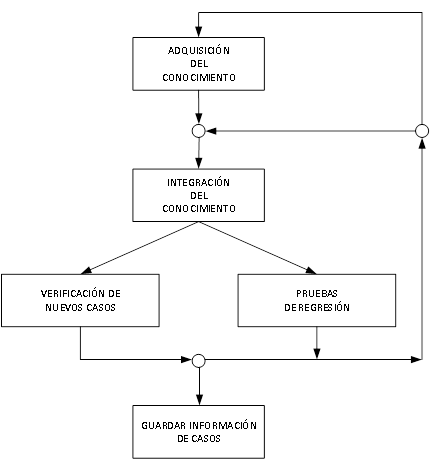
\includegraphics[scale=0.8]{chapters/chapter10/figures/10-4}
\caption{Implementación del conocimiento básico (Adaptado de (Rolston et al., 1990)).}
\label{fig:10-4}
\end{figure}
Como se ha insistido, la base de conocimiento es una reflexión cuidadosa del área en el momento en que el sistema se pone en servicio. Pero en muchas áreas complejas el conocimiento crece y cambia constantemente por lo cual la base de conocimientos de bebe modificar en el mismo sentido. Para llevar a cabo tales actualizaciones se emplean la facilidad para actualización de conocimientos. Este módulo puede tomar una de tres formas fundamentales (Rolston et al., 1990), según como se describe a continuación.\\
La primera forma, y también la más primitiva, es la actualización manual de conocimientos. En este caso la actualización se lleva a cabo por un IC quien interpreta la información ofrecida por un experto en el área y actualiza la base de conocimientos mediante el uso de un sistema limitado de actualización. \\
En la segunda forma, mucho más ambiciosa y prometedora, el experto en el área ingresa directamente el conocimiento revisado sin la mediación de un ingeniero  de conocimientos. En este caso el sistema de actualización de conocimientos debe ser mucho más elaborado.\\
En la tercera forma, donde se encuentra la frontera del conocimiento en este campo, el sistema genera nuevos conocimientos en forma automática y se basa en generalizaciones deducidas de experiencias anteriores. El sistema aprende nominalmente de la experiencia y se espera que el mismo sistema se actualice. Este proceso, se han logrado algunos buenos avances pero que aún está muy lejos de excelentes resultados, es tema de mucha investigación. La habilidad para aprender es un componente importante de la inteligencia y al ofrecer completamente esta potencialidad mejoraría las capacidades de un SE.\\
De esta manera, de forma ideal, puede afirmarse que en un SE ideal, el motor de inferencia nunca debería necesitar de modificaciones. En consecuencia, todas las mejoras al sistema de conocimientos se implementan mediante la expansión de la base de conocimientos. Sin embargo, según (Rolston et al., 1990), es raro que sea posible el asegurar una completa independencia de la base de conocimientos y del motor de inferencia.\\
\subsection{	Sistema de explicaciones}
Además de lograr simplemente una conclusión cuando se enfrenta un problema complicado, un experto también debe ser capaz de explicar lo cual implica comprender, hasta cierto punto, el razonamiento que conduce a dicha conclusión. Un SE debe diseñarse para brindar una facultad semejante. Esta es una potencialidad que generalmente está ausente en los sistemas tradicionales de computación pero que conforme pasa el tiempo se van convirtiendo en parte de las actuales soluciones informáticas (no necesariamente un SE).\\
Comúnmente, análogo a como se demuestra un teorema en el campo de las matemáticas,  la explicación consiste en una identificación de los pasos en el proceso de razonamiento y de una justificación de cada uno de ellos.  El implementar esta potencialidad para comunicar esta información, constituye esencialmente un subconjunto del problema del procesamiento de lenguaje natural. El sistema debe acceder a un registro de los conocimientos que se emplearon en el procesamiento, basándose en el esquema de representación de la base de conocimientos y traducirlo a una forma que sea aceptable y (principalmente) comprensible para el usuario.\\
Por lo tanto,  la credibilidad que se le concede a un SE, como ocurre también entre los humanos, depende de la habilidad del SE para explicar su propio proceso de razonamiento.  Reiterando, una persona experta también puede ser capaz de explicar sus razonamientos en forma adecuada al nivel de experiencia del que escucha. Un gerente de perforación de un pozo petrolero podría explicar a sus superiores que la perforación se ha cancelado debido a que los resultados de un reciente estudio sobre el terrero indica que la probabilidad de que ahí haya petróleo es de apenas 0.0005. \\
En consecuencia, para proporcionar los niveles críticos de explicación, el sistema debe identificar el nivel de conocimientos del usuario y entender cómo adaptar la explicación para acoplarla apropiadamente. Aún hoy en día con los desarrollos alcanzados, las facilidades de explicación en varios sistemas actuales se limitan a listar simplemente las reglas que se utilizaron durante la ejecución y son incapaces de justificar la razón.\\
\section{	LENGUAJES DE PROGRAMACIÓN PARA SISTEMAS EXPERTOS}
Por lo general, al desarrollar sistemas expertos la programación se centra en los temas de inferencia y búsqueda heurística y depende esencialmente de la manipulación de símbolos: series de caracteres. Los lenguajes de programación tradicionales para estas tareas son por excelencia LISP y PROLOG.  Estos lenguajes son los más empleados en la construcción de SE, aunque muchos lenguajes convencionales específicamente C, JAVA, Python entre otros, han cobrado mucha relevancia en el mundo contemporáneo.\\
El procesamiento simbólico es importante en SE, debido a que las primitivas de conocimiento en una base de conocimientos y las relaciones entre las primitivas de conocimientos, se almacenan mediante el uso de representaciones simbólicas. Es útil que los lenguajes de programación para SE puedan tratar libremente con ``cosas``, sin estar comprometido con la composición de dichas cosas.\\
\begin{figure}[H]
\centering
\captionsetup{justification=centering,margin=2cm}
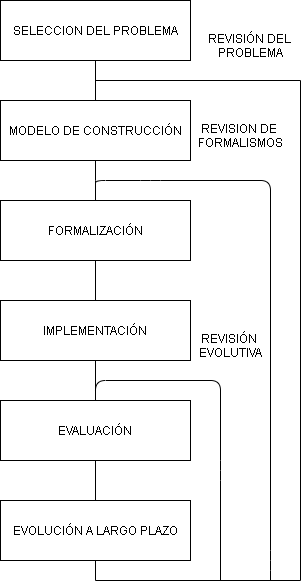
\includegraphics[scale=0.4]{chapters/chapter10/figures/1-5}
\caption{Ciclo de vida en la construcción de un SE (Adaptado de (Rolston et al., 1990).}
\label{fig:10-5}
\end{figure}
Una idea prometedora y no descabellada pero eso si compleja consiste en desarrollar primero el lenguaje de programación sobre el cual se desarrollará todo el sistema.  Esto debido a que ni LIST ni PROLOG  cuentan con herramientas adecuadas para manejar e inferir conocimiento de tipo difuso como fue propuesto para este proyecto.  Por esa razón puede pensarse en construir la herramienta (lenguaje de programación) con base en el cual se edificará la solución propuesta.\\
Cabe destacar que para lograrlo no solamente se debe emplear el paradigma de programación lógico sino que es fundamentar incorporar las capacidades de manejo de Objeto, eventos, programación distribuida, etc. También vale decir que no se trata de evitar el uso de lenguajes de programación que han mostrado sus grandes virtudes en el desarrollo de soluciones informáticas contemporáneas sino, más bien, construir un complemento de ellas para el caso particular en el que las herramientas existentes son débiles.\\
\section{ETAPAS DE DESARROLLO DE SISTEMAS EXPERTOS}
El proceso de desarrollo de SE, descrito en la Figura \ref{fig:10-5}, consiste de varias etapas básicas que son similares a las etapas típicas del ciclo de vida en ingeniería de software. La construcción de un SE es la construcción de un software y en ese sentido, las metodologías de desarrollo de aplicaciones es válida para este caso; sin embargo, el desarrollo de un SE tiene particularidades que lo diferencial del resto de programas por esa razón se hace necesario adaptar las metodologías y tener el debido cuidado al momento de emplearlas para este tipo de soluciones.\\
En general, estas etapas de construcción de un SE son (Rolston et al., 1990): \textbf{identificación del problema, construcción de un prototipo, formalización, implantación, evaluación y evolución a largo plazo}. La primera la  tarea en el desarrollo de cualquier SE, cuya estructura se esboza en Figura \ref{fig:10-3}, es establecer que el problema propuesto sea apropiado y requiera ser solucionado mediante un SE. Si el problema en consideración se puede describir en términos de definiciones y algoritmos explícitos, probablemente sea preferible desarrollar la solución de programación tradicional. Si el problema no está bien identificado o demanda amplio criterio humano (toma de decisiones de impacto ambiental y estabilidad financiera de las compañías, fijar políticas y establecer estrategias o juzgar la bondad en el bienestar de alguna estrategia), es probable que sea apropiado (aunque hay que tener cuidado) complejo para un SE.
\begin{figure}[H]
\centering
\captionsetup{justification=centering,margin=2cm}
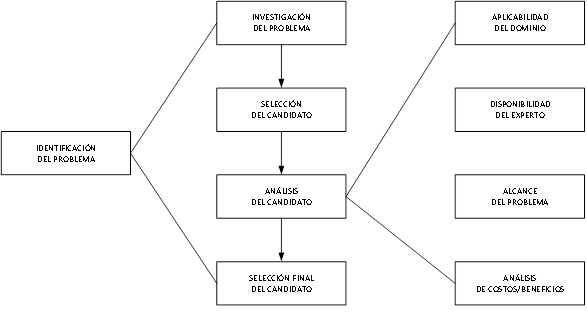
\includegraphics[scale=0.8]{chapters/chapter10/figures/10-6}
\caption{Identificación de problema}
\label{fig:10-6}
\end{figure}
Una vez el problema se ha seleccionado, se construye un prototipo pequeño para ayudar en la comprensión del problema completo y estimar la tarea de la construcción de la solución total. El siguiente paso en el proceso de desarrollo, es formalizar el enunciado del problema y diseñar completamente el SE.  En este punto del proceso se implementan y se interconectan todos los módulos de la Figura \ref{fig:10-7}.  Después de la formalización se realiza la implantación. Esto consiste principalmente de un ciclo continuo de adquisición de conocimientos, actualización de la base de conocimientos y pruebas.  Aquí es importante la selección de las herramientas de desarrollo que debería incluir la construcción de un lenguaje de programación para tal fin.\\
Por último, en la fase de evaluación, que sigue a la implantación, la estimación de la proximidad del sistema al desempeño experto. Después de la evaluación y entrega, el SE entra a un periodo de evolución a largo plazo. Durante este periodo el sistema continúa incrementado su competencia (según la experiencia que se vaya logrando con su empleo) y se revisa como respuesta a los cambios en los conocimientos del área. \\
Evidentemente es un sistema de alta complejidad pero, de la misma manera, puede decirse que la ingeniaría colombiana está preparada para su implementación.  Se requiere voluntad, tiempo suficiente y  recursos que permitan su realización.\\
\begin{figure}[H]
\centering
\captionsetup{justification=centering,margin=2cm}
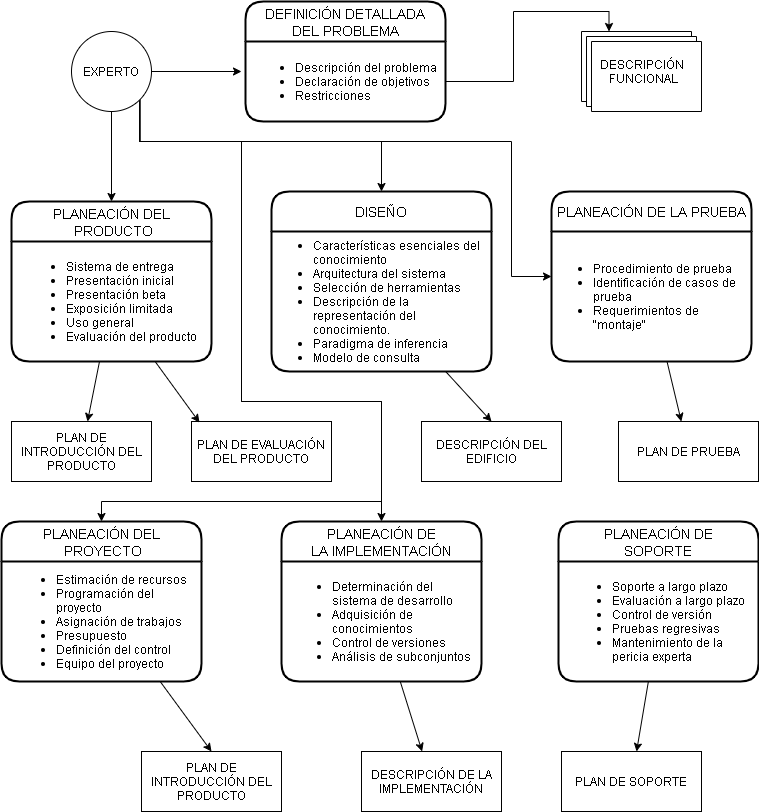
\includegraphics[scale=0.4]{chapters/chapter10/figures/1-7}
\caption{Formalización del SE (Adaptado de (Rolston et al., 1990)).}
\label{fig:10-7}
\end{figure}
Una observación que vale la pena subrayar antes de terminar el capítulo es que el sistema de control difuso que se propone en la capa más alta de toda la evolución del proyecto MIA, es, en sí mismo, un sistema experto.\\



\bibliographystyle{plain}
\bibliography{bibtex}

\printindex

\end{document}
